% https://nuanceabounds.org/fix-latex-package-option-clash-error-passoptionstopackage/
\PassOptionsToPackage{dvipsnames}{xcolor}

\documentclass{report}

% https://es.overleaf.com/learn/latex/Page_size_and_margins
\usepackage{geometry}
\geometry{
    %a4paper,
    top=25mm,
    bottom=25mm
}

% Font
\usepackage[T1]{fontenc}
% https://es.overleaf.com/learn/latex/Font_sizes%2C_families%2C_and_styles
\renewcommand{\familydefault}{\sfdefault}

% Saltear indentación en los párrafos
% https://tex.stackexchange.com/questions/14375/how-to-disable-automatic-indentation-on-new-paragraphs
\usepackage{parskip}

% Matemática
\usepackage{amsmath}    % símbolos matemáticos
\usepackage{amssymb}    % símbolos matemáticos
\usepackage{amsthm}     % teoremas
\usepackage{amsfonts}   % \mathbb
\usepackage{bm}         % bold math (https://ctan.org/pkg/bm)
\usepackage{abraces}    % \aunderbrace y \aoverbrace
% https://tex.stackexchange.com/questions/132526/overbrace-and-underbrace-with-square-bracket
\usepackage{mathtools}  % \mathclap
\usepackage{stmaryrd}   % \llbracket, \rrbracket

% Para hacer derivaciones y eso
% https://personal.utdallas.edu/~hamlen/trfrac.pdf
\usepackage{tfrac}

% Figuras
\usepackage{tikz}                   % gráficos
\usepackage{float}                  % [H]
\usepackage{xcolor}                 % colores https://es.overleaf.com/learn/latex/Using_colours_in_LaTeX

\usepackage{framed}     % textbars

\usepackage{graphicx} % Imagenes
\graphicspath{img/}

% Texto
\usepackage[shortlabels]{enumitem}  % enumerate con letras

% Referencias
\usepackage[colorlinks=true]{hyperref}

% https://tex.stackexchange.com/questions/121865/nameref-how-to-display-section-name-and-its-number
\newcommand*{\fullref}[1]{\hyperref[{#1}]{\autoref*{#1} \nameref*{#1}}}

% Programas
% https://tex.stackexchange.com/questions/116595/highlighting-haskell-listings-in-large-tex-document
% https://leportella.com/minted-vscode/
% https://tex.stackexchange.com/questions/367332/minted-error-undefined-control-sequence-pyg-with-texmaker
\usepackage[cache=false]{minted}     % código

% https://tex.stackexchange.com/questions/260566/how-to-reliably-switch-the-highlighting-color-with-soul
%\usepackage{soul}
%\DeclareRobustCommand{\hlcyan}[1]{{\sethlcolor{cyan}\hl{#1}}}


\usetikzlibrary{arrows,positioning,automata,shadows,fit,shapes}

% Teoremas, corolarios, etc.
% https://www.overleaf.com/learn/latex/theorems_and_proofs
\theoremstyle{definition} % Para que no salga en italicas

\newtheorem{theorem}{Teorema}[chapter]
\newtheorem*{theorem*}{Teorema}

\newtheorem{lemma}{Lema}[chapter]
\newtheorem*{lemma*}{Lema}

\newtheorem{proposition}{Prop.}[chapter]
\newtheorem*{proposition*}{Prop}

\newtheorem{definition}{Def.}[chapter]
\newtheorem*{definition*}{Def}

\newtheorem{observation}{Obs.}[chapter]
\newtheorem*{observation*}{Obs}

\newtheorem{example}{Ejemplo}[chapter]
\newtheorem*{example*}{Ejemplo}

% https://tex.stackexchange.com/questions/118173/how-to-write-ceil-and-floor-in-latex
\DeclarePairedDelimiter\ceil{\lceil}{\rceil}
\DeclarePairedDelimiter\floor{\lfloor}{\rfloor}

% Comandos de PLP
%\newcommand{\sigmatsequence}{\overset{\rightarrow}{\sigma}}
%\newcommand{\tautsequence}{\overset{\rightarrow}{\tau}}

% Entornos
\newenvironment{nota}[1]
    {\begin{leftbar}\textbf{#1}}
    {\end{leftbar}}

% https://tex.stackexchange.com/questions/42619/x-mark-to-match-checkmark/42620
\usepackage{pifont} % http://ctan.org/pkg/pifont
\newcommand{\cmark}{\ding{51}}
\newcommand{\xmark}{\ding{55}}

% Texto
\newcommand{\todo}[1]{{\textcolor{red}{\textbf{#1}}}}

% Mate general
\newcommand{\eqdef}{\overset{\text{def}}{=}}
\newcommand{\aeq}{=_\alpha}
\newcommand{\naeq}{\neq_\alpha}

% Calculo lambda
\newcommand{\extendTypesWith}[1]{\sigma ::= \dots \mid #1}
\newcommand{\lambdab}{\lambda^b}

\newcommand{\tfunc}[2]{#1 \to #2}
\newcommand{\ifte}[3]{\ \text{if } #1 \text{ then } #2 \text{ else } #3}
\newcommand{\abs}[3]{\lambda #1 : #2 . #3}
\newcommand{\app}[2]{#1 \ #2} % aplicación
\newcommand{\sustOne}[3]{#1 \{ #2 \leftarrow #3 \}}

\newcommand{\uabs}[2]{\lambda #1 . #2} % untyped

\newcommand{\tipa}[3]{#1 \rhd #2 : #3} % \vartriangleright
\newcommand{\tienetipo}[3]{#1 : #2 \in #3}
\newcommand{\Gtipa}[2]{\tipa{\Gamma}{#1}{#2}}
\newcommand{\GStipa}[2]{\tipa{\Gamma|\Sigma}{#1}{#2}}
\newcommand{\compat}[2]{#1 \rhd #2} % compatibilidad
\newcommand{\GSCompat}[1]{\compat{\Gamma|\Sigma}{#1}} % compatibilidad

\newcommand{\fv}[1]{\text{FV}(#1)} % free vars
\newcommand{\bv}[1]{\text{BV}(#1)} % bound vars (ligadas)

% Lambda bn
\newcommand{\lambdabn}{\lambda^{bn}}
\newcommand{\suc}[1]{succ(#1)}
\newcommand{\pred}[1]{pred(#1)}
\newcommand{\iszero}[1]{iszero(#1)}
\newcommand{\num}[1]{\underbar{#1}} % abreviación de suc^#1(0)

% Lambda reg
\newcommand{\lambdareg}{\lambda^{\dots r}}
\newcommand{\reg}[1]{\{\ #1\ \}}
\newcommand{\proj}[2]{#1 . #2}

\newcommand{\treg}[1]{\{ #1 \}}

\newcommand{\iesimo}[1]{#1_i^{\ \ i \in 1..n}}

% Lambda bnu
\newcommand{\lambdabnu}{\lambda^{bnu}}
\newcommand{\seq}[2]{#1;#2}

% Lambda let
\newcommand{\lambdalet}{\lambda^{\dots let}}
\newcommand{\letin}[4]{\text{let } #1 : #2 = #3 \text{ in } #4}
\newcommand{\uletin}[3]{\text{let } #1 = #2 \text{ in } #3} % untyped
\newcommand{\alloc}[1]{\text{ref } #1}
\newcommand{\dealloc}[1]{!#1}
\newcommand{\assign}[2]{#1 := #2}

\newcommand{\unit}{unit}
\newcommand{\tunit}{Unit}

\newcommand{\tref}[1]{\text{Ref } #1}

\newcommand{\dom}[1]{Dom(#1)}

\newcommand{\store}[3]{#1 [#2 \mapsto #3]}
\newcommand{\estore}[3]{#1 \oplus (#2 \mapsto #3)}
\newcommand{\mustore}[2]{\store{\mu}{#1}{#2}}
\newcommand{\emustore}[2]{\estore{\mu}{#1}{#2}}

\newcommand{\mematSet}[3]{#1(#2) = #3}
\newcommand{\memat}[2]{#1(#2)}

\newcommand{\sreduce}[4]{\reduce{#1\mid#2}{#3\mid#4}}
\newcommand{\sreduceToPrime}[2]{\sreduce{#1}{#2}{#1'}{#2'}}

\newcommand{\sreducesTo}[5]{#1\mid#2 \reducesTo{#3} #4\mid#5}
\newcommand{\expstore}[2]{#1 \mid #2}

% Recursión
\newcommand{\fix}[1]{\text{fix } #1}
\newcommand{\letrec}[4]{\text{letrec } #1 : #2 = #3 \text{ in } #4}

% Reducciones
\newcommand{\reduces}{\to}
\newcommand{\reducesTo}[1]{\reduces_\text{(#1)}}
\newcommand{\reduce}[2]{#1 \reduces #2}
\newcommand{\reduceToPrime}[1]{\reduce{#1}{#1'}}
\newcommand{\doesntReduce}[2]{#1 \not\reduces #2}

\newcommand{\reduceManyTo}{\twoheadrightarrow}
\newcommand{\reduceMany}[2]{#1 \reduceManyTo #2}

\newcommand{\deriv}[3]{\trfrac[(#1)]{#2}{#3}}
\newcommand{\derivok}[1]{\trfrac[]{\checkmark}{#1}}
\newcommand{\ederiv}[2]{\trfrac{#1}{#2}} % empty deriv

% Para indicar que algo se conv en valor
\newcommand{\changed}[1]{\textcolor{Red}{#1}}
\newcommand{\select}[1]{\textcolor{Blue}{#1}}
\newcommand{\green}[1]{\textcolor{OliveGreen}{#1}}

\newcommand{\evalsto}{\leadsto}

% Inferencia
\newcommand{\untypedTerms}{\Lambda}
\newcommand{\typedTerms}{\Lambda_\tau}
\newcommand{\typeVars}{\mathcal{V}}
\newcommand{\types}{\mathcal{T}}
\newcommand{\erase}[1]{\text{Erase}(#1)}

\newcommand{\tsust}[1]{S#1} % apply type sust
\newcommand{\sustfor}[2]{#1/#2} % type sust

\newcommand{\GTipaInst}[2]{\tipa{\Gamma'}{#1'}{#2'}} % instancia

\newcommand{\infer}[1]{\mathbb{W}(#1)}

\newcommand{\tcontextOne}[2]{\{ #1 : #2 \}} % type context
\newcommand{\etipa}[2]{\tipa{\emptyset}{#1}{#2}} % emptyset tipa

\newcommand{\comp}[2]{#1 \circ #2}
\newcommand{\unify}[2]{#1 \doteq #2}

\newcommand{\unifySetD}{\{
    \unify{\sigma_1}{\sigma_1'},
    \dots,
    \unify{\sigma_n}{\sigma_n'} 
\}}

%% Unificación
\newcommand{\simpSust}[1]{\mapsto_{#1}}
\newcommand{\simp}{\mapsto}

\newcommand{\asimpSust}[2]{\mapsto_{#2}^{#1}} % annotated
\newcommand{\asimp}[1]{\mapsto^{#1}}

\newcommand{\mgu}[2]{\text{MGU}(\{ \unify{#1}{#2} \})}

% Subtipado
\newcommand{\subt}[2]{#1 <: #2}

\newcommand{\ligada}[1]{\underbrace{#1}_{\text{ligada}}}
\newcommand{\libre}[1]{\underbrace{#1}_{\text{libre}}}

\newcommand{\tsource}[1]{\text{Source } #1}
\newcommand{\tsink}[1]{\text{Sink } #1}

\author{Manuel Panichelli}
\title{Notas para final de PLP}

\begin{document}

\maketitle

\tableofcontents

\chapter{Paradigma funcional}

\section{Haskell}

\begin{definition}[Paradigma]
    Un \textbf{paradigma} es una forma de pensamiento.
\end{definition}

\begin{definition}[Lenguaje de programación]
    Un \textbf{lenguaje de programación} es el lenguaje que usamos para
    comunicar lo que queremos que haga una computadora.

    Usamos un lenguaje para describir los computos que lleva a cabo la
    computadora.
    
    Es \textbf{computacionalmente completo} si puede expresar todas las
    funciones computables. Hay DSLs (\textit{domain specific languages}) que no
    pueden expresar todo lo computable.
\end{definition}

\begin{definition}[Paradigma de lenguaje de programación]
    Lo entendemos como un \textit{estilo} de programación, que tiene que ver con
    los estilos de las soluciones. Está vinculado con lo que es para uno un
    modelo de cómputo.

    Lo que vemos antes de la materia es el imperativo: a partir de un estado
    inicial llegar a un estado final. Programamos con secuencias de
    instrucciones para cambiar el estado.
\end{definition}

\subsection{Programación funcional}

Definiciones:

\begin{itemize}
    \item \textbf{Programa y modelo de cómputo}: Programar es definir
    funciones, y ejecutar es evaluar expresiones.
    \item \textbf{Programa}: Es un conjunto de ecuaciones. Por ej.
    \texttt{doble x = x + x}
    \item \textbf{Expresiones}: El significado de una expresión es su valor
    (si es que está definido). El valor de una expresión depende solo del
    valor de sus sub-expresiones. Evaluar o reducir una expresion es obtener
    su valor (por ej. \texttt{doble 2 $\leadsto$ 4})
    No toda expresion denota un valor, por ejemplo \texttt{doble true}.
    \item \textbf{Tipos}: El universo de valores está particionado en
    colecciones denominadas \textit{tipos}, que tienen operaciones asociadas.
\end{itemize}

Haskell es \textbf{fuertemente tipado}. Toda expresion bien formada tiene un
tipo, que depende del tipo de sus subexpresiones. Si no puede asignarse un tipo
a una expresión, no se la considera bien formada.

\begin{minted}{haskell}
1           :: Int
'a'         :: Char
1.2         :: Float
True        :: Bool
[1, 2, 3]   :: [Int]
(1, True)   :: (Int, Bool)
succ        :: Int -> Int
\end{minted}

Definiciones de funciones:

\begin{minted}{haskell}
-- Definición
doble :: Int -> Int
doble x = x + x

-- Guardas
signo :: Int -> Bool
signo n | n >= 0    = True
        | otherwise = False

-- Definiciones locales
f (x, y) = g x + y
    where g z = z + 2

-- Expresiones lambda
\x -> x + 1
\end{minted}

\textbf{Tipos polimórficos}

\begin{minted}[]{haskell}
    id x = x
    id :: a -> a
    -- x es de tipo a, que eventualmente se va a instanciar a algún tipo
\end{minted}

\textbf{Clases de tipos}: Son como interfaces, que definen un conjunto de
operaciones.

\begin{minted}[]{haskell}
    maximo :: Ord a => a -> a -> a
    maximo x y | x > y = x
    maximo _ y = y
    -- Ord: (<), (<=), (>=), (>), max, min, compare
\end{minted}

\textbf{Tipos algebráicos}

\begin{minted}[]{haskell}
    data Figura = Circulo Float | Rectangulo Float Float
    deriving Eq -- deriva la igualdad nativa

    -- (Circulo 1) == (Circulo 1)
\end{minted}

Estas cosas nos permiten hacer funciones genéricas.

\textbf{Funciones de alto orden}: las funciones son first class citizens, se
pueden pasar como parámetro.

\subsection{Currificación}

Es un mecanismo que permite reemplazar argumentos estructurados por una
secuencia de argumentos "simples". Ventajas:

\begin{itemize}
    \item Evaluación parcial: \texttt{succ = suma 1}
    \item Evita escribir paréntesis (asumiendo que la aplicación asocia a
    izquierda). \texttt{suma 1 2 = ((suma 1) 2)}
\end{itemize}

\begin{nota}
    Por ejemplo, si definimos
    \begin{minted}{haskell}
    add (x, y) = x + y
    \end{minted}
    no está currificada, ya que recibe sus argumentos todos juntos. En cambio,
    \begin{minted}{haskell}
    add x y = x + y
    \end{minted}
    si está currificada.

    Esto es porque escribir \texttt{add x y = x + y} es una conveniencia, pero 
    lo que en realidad pasa por debajo es
    
    \begin{minted}{haskell}
        add x y = x + y
        add x = \y -> x + y
        add = \x -> (\y -> x + y)
    \end{minted}

    De esa forma, cada aplicación de un argumento devuelve una función, que
    podría ser aplicada de vuelta o no (y ahí tenemos aplicación parcial)
\end{nota}

\textbf{curry y uncurry}

En criollo: una equivalencia entre una func con muchos parametros (una tupla) y
una funcion equivalente que va tomando de a uno y devuelve funciones.

\begin{minted}[]{haskell}
    curry :: ((a, b) -> c) -> (a -> (b -> c))
    curry f a b = f (a, b)

    suma x y = x + y
    suma' :: (Int, Int) -> Int
    suma' (x, y) = x + y

    curry suma' 1 2 = suma' (1, 2)
    curry suma' :: (Int -> (Int -> Int))

    uncurry :: (a -> b -> c) -> ((a -> b) -> c)
    uncurry f (a, b) = f a b
\end{minted}

\subsection{Pattern matching}

Una forma copada de definir funciones. Es un mecanismo para comparar un valor
con un patrón. Si la comparación tiene éxito se puede deconstruir un valor en
sus partes.

\begin{minted}[]{haskell}
    data Figura = Circulo Float | Rectangulo Float Float

    area :: Figura -> Float
    area (Circulo radio) = pi * radio ^ 2
    area (Rectangulo l1 l2) = l1 * l2
\end{minted}

El patrón está formado por el constructor y las variables. Los casos se evalúan
en el orden en el que están escritos.

\begin{minted}[]{haskell}
    esCuadrado :: Figura -> Bool
    -- También vale esto
    -- esCuadrado (Rectangulo x y) = (x == y)
    esCuadrado (Rectangulo x y) | (x==y) = True
    esCuadrado _ = False
\end{minted}

También se pueden definir funciones parciales (que no estén definidas para todo
el dominio).

\subsection{Tipos recursivos}
La definición de un tipo puede tener uno o más parámetros del tipo

\begin{minted}[]{haskell}
    data Natural = Zero | Succ Natural

    Zero :: Natural                     -- 0
    succ Zero :: Natural                -- 1
    succ (succ (succ Zero)) :: Natural  -- 2

    dameNumero :: Natural -> Int
    dameNumero Zero = 0
    dameNumero (Succ n) = dameNumero n + 1
\end{minted}

\subsection{Listas}

Tipo algebráico paramétrico recursivo con dos constructores:

\begin{minted}[]{haskell}
    [] :: [a]               -- lista vacia
    (:) :: a -> [a] -> [a]  -- constructor infijo

    -- Ejemplo
    --   1 : [2, 3] = [1, 2, 3]
\end{minted}

Pattern matching

\begin{minted}[]{haskell}
    vacia :: [a] -> Bool
    vacia [] = True
    vacia _ = False

    long :: [a] -> Int
    long [] = 0
    long x:xs = 1 + long xs
\end{minted}

\subsection{No terminación y orden de evaluación}

\begin{minted}[]{haskell}
    -- No terminación
    inf1 :: [Int]
    inf1 = 1 : inf1

    -- Evaluación no estricta
    const :: a -> b -> a
    const x y = x

    -- const 42 inf1 -> 42 (pero depende del mecanismo de reducción del
    -- lenguaje)
\end{minted}

\subsection{Evaluación lazy}

el modelo de cómputo de haskell es la \textbf{reducción}. Se reemplaza un
\textit{redex} por otro usando las ecuaciones orientadas. Un redex (reducible
expression) es una sub-expresión que no está en forma normal (irreducible).

Un redex debe ser una \textbf{instancia} del lado izquierdo de alguna ecuación y
será reemplazado por el lado derecho con las variables correspondientes ligadas.
El resto de la expresión no cambia.

Haskell hace esto hasta llegar a una forma normal, un valor irreducible.

\texttt{const x y = x}. \texttt{const x y} es un redex, y lo reduzco a
\texttt{x}.

Y cómo selecciono una redex? \textbf{Orden normal} (lazy). Se selecciona el
redex más externo para el que se pueda conocer que ecuación del programa
utilizar. En general, primero las funciones más externas y luego los argumentos,
solo de ser necesarios.

Modo aplicativo: reduce primero todos los argumentos. Se hace en otros lenguajes
como c.

\subsection{Esquemas de recursion}

Formas de recursion comunes que uno puede aprovechar usando funciones de alto
orden.

\subsubsection{Map}

\begin{minted}[]{haskell}
-- tal que dobleL xs es la lista que contiene el doble de cada elemento en xs
dobleL :: [Float] -> [Float]
dobleL [] = []
dobleL (x:xs) = 2*x : dobleL xs

-- tal que la lista esParL xs indica si el correspondiente elemento en xs es par
-- o no
esParL :: [Int] -> [Bool] 
esParL [] = []
esParL (x:xs) = (even x) : esParL xs

-- tal que longL xs es la lista que contiene las longitudes de las listas en xs
longL :: [[a]] -> [Int]
longL [] = []
longL (x:xs) = (length x) : longL xs

-- esquema recursivo de map:
map :: (a -> b) -> [a] -> [b]
map _ [] = []
map g (x:xs) = g x : map g xs

-- Con eso, se pueden reescribir como
dobleL = map ((*) 2)
esParL = map even
longL = map length
\end{minted}

\subsubsection{Filter}

\begin{minted}{haskell}
-- tal que negativos xs contiene los elementos negativos de xs
negativos :: [Float] -> [Float]
negativos [] = []
negativos (x:xs)
    | x < 0 = x : (negativos xs)
    | otherwise = negativos xs

-- tal que la lista noVacias xs contiene las listas no vacias de xs
noVacias :: [[a]] -> [[a]]
noVacias [] = []
noVacias (l:ls)
    | (length l > 0) = l : (noVacias ls)
    | otherwise = noVacias ls

-- esquema recursivo:
filter :: (a -> Bool) -> [a] -> [a]
filter _ [] = []
filter p (x:xs) = if (p x) then x : (filter p xs)
                  else (filter p xs)

-- luego quedan
negativos = filter (\x -> x < 0)
noVacias = filter (\l -> length l != 0)
noVacias = filter ((> 0) . length) -- f o g = f(g(x))

\end{minted}

\subsection{Transparencia referencial}

El valor de una expresion en funcional depende solo de sus subexpresiones. Esto
a diferencia de imperativo que depende del estado.

Si dos expresiones son iguales, denotan el mismo valor bajo el mismo contexto.

\subsection{Folds}

\subsubsection{foldr}

\begin{minted}[]{haskell}
-- Funciones sobre listas
-- Motivación: Como estas funciones cambian la forma de lo que devolvemos, no lo
-- podemos hacer con map o filter.

-- sumaL: suma de todos los valores de una lista de enteros
sumaL :: [Int] -> Int
sumaL [] = 0
sumaL (x:xs) = x + (sumaL xs)

-- concat: la concatenación de todos los elementos de una lista de listas
concat :: [[a]] -> [a]
concat [] = []
concat (l:ls) = l ++ (concat ls)

-- reverso: el reverso de una lista
reverso :: [a] -> [a]
reverso [] = []
reverso (x:xs) = (reverso xs) ++ [x]

-- Esquema de recursión
foldr :: (a -> b -> b) -> b -> [a] -> b
foldr _ z [] = z
foldr f z (x:xs) = f x (foldr f z xs)

-- Luego, con esto
sumaL = foldr (+) 0
concat = foldr (++) []
reverso = foldr (\x rec -> rec ++ [x]) []
reverso = foldr ( (flip (++)) . (:[])) []

-- Hasta podemos definir map y filter. El fold es más general que el map y
-- filter
map f = foldr (\x rec -> f x : rec) []
map f = foldr ((:) . f) []

-- (:) . f :: a -> [b] -> [b]
-- ((:) . f) x  = (f x) :

filter p = foldr (\x rec -> if p x then x : rec else rec) []

-- Longitud y suma con una sola pasada sobre la lista
sumaLong :: [Int] -> (Int, Int)
sumaLong = foldr (\x (rl, rn) -> (rl + 1, rn + x)) (0, 0)
\end{minted}

Definición de \texttt{++}
\begin{minted}{haskell}
    (++) :: [a] -> [a] -> [a]
    xs ++ ys = foldr (:) ys xs
\end{minted}

\begin{center}
    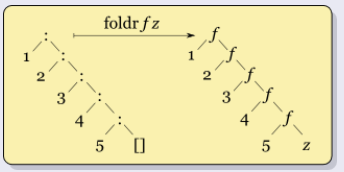
\includegraphics[scale=0.6]{img/funcional/foldr.png}
\end{center}

\subsubsection{recr}

\begin{minted}[]{haskell}
-- dropWhile
dropWhile :: (a -> Bool) -> [a] -> [a]
dropWhile _ [] = []
dropWhile p (x:xs) = if p x then dropWhile p xs else x:xs

-- ejemplo
dropWhile even [2, 4, 1, 6] = [1, 6]

-- drop while cuando se termina de cumplir devuelvo todo lo que viene "a la
-- derecha", pero cuando hago fold, lo que está a la derecha ya pasó por la
-- recursión.
-- Para poder hacerlo con foldr, nos guardamos la lista además de la recursión y
-- en cada paso decidimos si quedarnos con la recursión (cosas dropeadas) o la
-- lista original

dropWhile' :: (a -> Bool) -> [a] -> ([a], [a])
dropWhile' p = foldr f ([], [])
    where f = (\x, (rs, os) -> if p x then rs else x: os)

dw p = first $ (foldr (\x (r1, r2)
    -> (if p x then r1 else x: r2, x: r2 ) ), ([], []))

\end{minted}

Podemos otro esquema más poderoso: \textbf{recursión primitiva}. En cada paso,
tengo acceso a la lista no modificada y la modificada.

\begin{minted}{haskell}
-- esquema
g :: [a] -> b
g [] = z
g (x:xs) = f x xs (g xs)

{-
g [1, 2, 3]
= f 1 [2, 3] (g [2, 3])
= f 1 [2, 3] (f 2 [3] (g [3]))
= f 1 [2, 3] (f 2 [3] (f 3 [] (g [])))
= f 1 [2, 3] (f 2 [3] (f 3 [] z))
-}

recr :: b -> (a -> [a] -> b -> b) -> [a] -> b
recr z _ [] = z
recr z f (x:xs) = f x xs (recr z f xs)

-- Con esto podemos reescribir dropWhile sin hacer nada raro
dropWhile p = recr [] (\x xs rec -> if p x then rec else x:xs)

-- foldr en terminos de recr? Alcanza con ignorar xs
foldr f z = recr z (\x xs rec -> f x rec)

-- recr en términos de foldr?
recr z f = first $
    foldr
        (\x (rs1, rs2) -> (f x rs2 rs1, x:rs2))
        (z, [])

recr z f = foldr f (z, [])
    where f = (\x, (rec, xs) -> f x xs rec)
\end{minted}

\subsubsection{foldl}

\begin{center}
    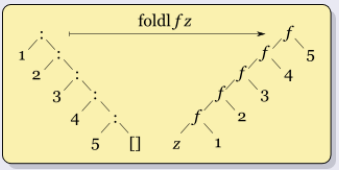
\includegraphics[scale=0.6]{img/funcional/foldl.png}
\end{center}

\begin{minted}[]{haskell}
    foldl :: (b -> a -> b) -> b -> [a] -> b
    foldl _ z [] = z
    foldl f z (x:xs) = foldl f (f z x) xs
\end{minted}

foldr = fold a la derecha, y foldl = fold a la izquierda

\begin{minted}[]{haskell}
reverse = foldl (\c x -> x:c) []
reverse = foldl (flip (:)) []
\end{minted}

Y uno en términos del otro? \textit{Me falta repasar esto porque estaba matado,
min 2:35:10 del video}

En listas infinitas, foldl se traba y foldr no. Esto es porque para terminar de
evaluar, foldl tiene que llegar hasta el final de la lista.

\subsubsection{Fold sobre estructuras algebrácias}

\begin{minted}[]{haskell}
-- Arbol binario
data Arbol a = Hoja a | Nodo a (Arbol a) (Arbol a)

-- Por ej.

Nodo 1 (Hoja 2) (Hoja 3)

-- Es
--
--   1
--  / \
-- 2   3

-- Y sobre ella podemos querer operaciones, como map

mapA :: (a -> b) -> Arbol a -> Arbol b
mapA f (Hoja x) = Hoja f x
mapA f (Nodo x izq der) = Nodo (f x) (mapA f izq) (mapA f der)

-- Y también podemos hacer un fold

foldA :: (a -> b) -> (a -> b -> b -> b) -> Arbol a -> b
foldA f g (Hoja x) = f x
foldA f g (Nodo x izq der) = g x (foldA f g izq) (foldA f g der)

sumaA = foldA id (\x rizq rder -> x + rizq + rder)
contarHojas = foldA 1 (\x rizq rder -> rizq + rder)

-- Por los tipos de los constructores, también podemos hacer la identidad
idA = foldrA (Hoja) (Nodo)

-- Arboles generales
data AG = NodoAG a [AG a]

mapAG :: (a -> b) -> AG a -> AG b
mapAG f (Nodo AG a as) -> NodoAG (f a) (map (mapAG f) as)

foldAG :: (a -> [b] -> b) -> AG a -> b
foldAG f (NodoAG a as) = f a (map (foldAG f) as)
\end{minted}

\textit{Aplicar un fold con un constructor es la identidad}.

\section{Cálculo Lambda Tipado}

Es el formalismo que está detrás de la programación funcional. Es un modelo de
cómputo basado en \textbf{funciones}, introducido por Alonzo Church en 1934. Es
computacionalmente completo (turing completo) y nosotros vamos a estudiar la
variante tipada (Church, 1941.)

La máquina de turing es más de estado, y este con reducción de expresiones.

\begin{definition}[Tipos]
    Las \textbf{expresiones de tipos} (o tipos) de $\lambdab$ (lambda cálculo b
    de booleano) son

    \[
        \sigma, \tau ::= Bool \mid \tfunc{\sigma}{\tau}
    \]

    Informalmente, 
    
    \begin{itemize}
        \item \textit{Bool} es el tipo de los booleanos, y
        \item $\tfunc{\sigma}{\tau}$ es el tipo de las funciones de tipo $\sigma$ en tipo $\tau$.
    \end{itemize}

    \begin{example*}
        Ejemplos:
        \begin{itemize}
            \item $\tfunc{Bool}{Bool}$
            \item $\tfunc{\tfunc{Bool}{Bool}}{Bool}$
        \end{itemize}
    \end{example*}
\end{definition}

\begin{definition}[Terminos]
    Los términos se escriben con las siguientes reglas de sintaxis.

    Sea $\chi$  un conjunto infinito enumerable de variables, y $x \in \chi$.
    Los \textbf{términos} de $\lambdab$ están dados por,

    \begin{align*}
        M, N, P, Q ::&= x \\
            &\mid \quad true \\
            &\mid \quad false \\
            &\mid \quad \ifte{M}{P}{Q} \\
            &\mid \quad \abs{x}{\sigma}{M} \\
            &\mid \quad \app{M}{N} \\
    \end{align*}

    \begin{example*} Ejemplos:
        \begin{itemize}
            \item $\abs{x}{Bool}{x}$ \cmark
            \item $\abs{x}{Bool}{\ifte{x}{false}{true}}$ \cmark
            \item
            $\abs{f}{\tfunc{Bool}{\tfunc{Bool}{Bool}}}{\abs{x}{Bool}{\app{f}{x}}}$
            \cmark
            \item $(\abs{f}{\tfunc{Bool}{Bool}}{\app{f}{true}})
            (\abs{y}{Bool}{y})$ \cmark
            \item $\app{true}{(\abs{x}{Bool}{x})}$ \cmark
            \item $\app{x}{y}$ \cmark
            \item $\lambda x : true$ \xmark
        \end{itemize}
    \end{example*}
\end{definition}

\subsection{Sistema de tipado}

Es un sistema formal de deducción o derivación que utiliza axiomas y reglas de
inferencia para caracterizar un subconjunto de los términos llamados
\textbf{tipados}. Nos permite quedarnos con algunos y rechazar otros términos en
base a lo que consideremos correcto.

Definimos una \textbf{relación de tipado} en base a reglas de inferencia.
\begin{itemize}
    \item Los \textbf{axiomas de tipado} establecen que ciertos \textbf{juicios
    de tipado} son derivables.
    \item Las \textbf{reglas de tipado} establecen que ciertos \textbf{juicios
    de tipado} son derivables siempre y cuando ceiertos otros lo sean.  
\end{itemize}

\begin{definition}[Variables libres]
Una variable puede ocurrir \textbf{libre} o ligada en un término. Decimos que
$x$ ocurre \textbf{libre} si no se encuentra bajo el alcance de una ocurrencia
de $\lambda x$. Caso contrario ocurre ligada.

Ejemplos:

\begin{itemize}
    \item $\abs
        {x}{Bool}
        {\ifte{\ligada{x}}{true}{false}}$
    \item $\abs
        {x}
        {Bool}
        {\abs{y}{Bool}{\ifte{true}{\ligada{x}}{\ligada{y}}}}$
    \item $\abs{x}{Bool}{\ifte{\ligada{x}}{true}{\libre{y}}}$
    \item $\app{(\abs{x}{Bool}{\ifte{\ligada{x}}{true}{false}})}{\libre{x}}$
\end{itemize}

La definición formal es a partir de cada término del lambda cálculo por pattern
matching. FV = Free Variable

\begin{align*}
    \fv{x} &\eqdef \{ x \} \\
    \fv{true} = \fv{false} &\eqdef \emptyset \\
    \fv{\ifte{M}{P}{Q}} &\eqdef \fv{M} \cup \fv{P} \cup \fv{Q} \\
    \fv{\app{M}{N}} &\eqdef \fv{M} \cup \fv{N} \\
    \fv{\abs{x}{\sigma}{M}} &\eqdef \fv{M} \setminus \{ x \}
\end{align*}
\end{definition}

\begin{definition}[Juicio de tipado]
    Un \textbf{juicio de tipado} es una expresión de la forma
    $\tipa{\Gamma}{M}{\sigma}$, que se lee \textit{``El término M tiene el
    tipo $\sigma$ asumiendo el contexto de tipado $\Gamma$''}.

    Un \textbf{contexto de tipado} es un conjunto de pares $x_i : \sigma_i$,
    notado $\{ x_1 : \sigma_1, \dots, x_n : \sigma_n \}$ donde los $x_i$ son
    distintos. Usamos las letras $\Gamma, \Delta, \dots$ para contextos de
    tipado.

    A las variables se les anota un tipo. Uno pone las asunciones que tiene
    sobre el tipo de algunas variables, como $x : Bool$.
\end{definition}

\begin{definition}[Axiomas de tipado de $\lambdab$]

Son guiadas por sintaxis al igual que las variables libres

\[
    \deriv{T-True}{}{\Gtipa{true}{Bool}} \quad
    \deriv{T-False}{}{\Gtipa{false}{Bool}}
\]

(para cualquier contexto de tipado $\Gamma$)

\[
    \deriv
        {T-Var}
        {\tienetipo{x}{\sigma}{\Gamma}}
        {\Gtipa{x}{\sigma}}
\]

\[
    \deriv
        {T-If}
        {
            \Gtipa{M}{Bool} \quad
            \Gtipa{P}{\sigma} \quad
            \Gtipa{Q}{\sigma}
        }
        {\Gtipa{\ifte{M}{P}{Q}}{\sigma}}
\]

P y Q tienen que tener el mismo tipo porque queremos que la expresion siempre
tipe a lo mismo.

\[
    \deriv
        {T-Abs}
        {\tipa{\Gamma, x : \sigma}{M}{\tau}}
        {\Gtipa{\abs{x}{\sigma}{M}}{\tfunc{\sigma}{\tau}}}
    \quad
    \deriv
        {T-App}
        {
            \Gtipa{M}{\tfunc{\sigma}{\tau}} \quad
            \Gtipa{N}{\sigma}
        }
        {\Gtipa{\app{M}{N}}{\tau}}
\]
\end{definition}

Si $\Gtipa{M}{\sigma}$ puede derivarse usando los axiomas y reglas de tipado,
decimos que es \textbf{derivable}, y decimos que $M$ es \textbf{tipable} si el
juicio de tipado $\Gtipa{M}{\sigma}$ puede derivarse para algún $\Gamma$ y
$\sigma$.

Ejemplos:

\begin{itemize}
    \item $\abs{x}{Bool}{x} : \textcolor{blue}{\tfunc{Bool}{Bool}}$
    
    \[
    \deriv
        {T-Abs}
        {
            \deriv
                {T-Var}
                {\derivok{x : Bool \in \Gamma'}}
                {
                    \tipa{\Gamma' = \Gamma \cap \{x : Bool\}}{x}{Bool}
                }
        }
        {\Gtipa{\abs{x}{Bool}{x}}{\textcolor{blue}{\tfunc{Bool}{Bool}}}}
    \]

    \item $\abs{x}{Bool}{\ifte{x}{false}{true}}$
    \item $\abs{f}{\tfunc{Bool}{\tfunc{Bool}{Bool}}}{\abs{x}{Bool}{\app{f}{x}}}$
    \item $(\abs{f}{\tfunc{Bool}{Bool}} \app{f}{true})(\abs{y}{Bool}{y})$
    \item $\app{true}{(\abs{x}{Bool}{x})}$. No va a tipar nunca, porque $true :
    Bool$ y para $T-App$ necesitamos que sea $\tfunc{\sigma}{\tau}$.
    \item $\app{x}{y}$. Para usar T-App, x por sintaxis solo aplica a T-Var. La
    única forma de que pueda aplicar x con y, x tiene que ser tipo flecha. Pero
    es una variable, entonces solo funcionaría si tenemos como asunción de tipo
    de x como función en $\Gamma$. Sin eso no se puede tipar.
\end{itemize}

\subsection{Resultados básicos}

\textit{Se pueden probar por inducción en la longitud de las reglas}

\begin{proposition}[Unicidad de tipos]
    Si $\Gtipa{M}{\sigma}$ y $\Gtipa{M}{\tau}$ son derivables, entonces $\sigma
    = \tau$.

    \textit{Si una expresión tiene un tipo, ese tipo es único.}
\end{proposition}

\begin{proposition}[Weakening + Strengthening]
    Si $\Gtipa{M}{\sigma}$ es derivable y $\Gamma \cap \Gamma'$ contiene a todas
    las variables libres de $M$, entonces $\tipa{\Gamma'}{M}{\sigma}$.

    \textit{Puedo agrandar o achicar el contexto de tipo siempre y cuando contenga las mismas variables libres.}
\end{proposition}

\subsection{Semántica}

Habiendo definido la sintaxis de $\lambdab$, nos interesa formular como se
\textbf{evalúan} o \textbf{ejecutan} los términos. Hay varias maneras de definir
\textbf{rigurosamente} la semántica de un lenguaje de programación, nosotros
vamos a definir una \textbf{semántica operacional}.

\begin{itemize}
    \item Denotacional. Darle una \textit{denotación} a cada símbolo del
    lenguaje, qué denota matemáticamente. Y uno define la semántica en términos
    de como las funciones van denotando cosas, con recursión o puntos fijos.
    \item Axiomática. Cuando cursamos algo1, definimos pre y pos condiciones.
    Predicaque definen el significado de una operación. Las triplas de hoare y
    esas cosas.
    \item \textbf{Operacional} consiste en
    \begin{itemize}
        \item interpretar a los \textbf{términos como estados} de una máquina
        abstracta, y
        \item definir una \textbf{función de transición} que indica dado un
        estado cuál es el siguiente. 
    \end{itemize}
\end{itemize}

El \textbf{significado} de un término $M$ es el estado final que alcanza la
máquina al comenzar con $M$ como estado inicial. Hay dos formas de definir
semántica operacional,

\begin{itemize}
    \item \textbf{Small-step}: la función de transición describe un paso de
    computación. Esta vamos a hacer nosotros.
    \item \textbf{Big-step} (o \textbf{Natural Semantics}): la función de
    transición, en un paso, evalúa el término a su resultado.
\end{itemize}

\begin{definition}[Juicios]
    La formulación se hace a través de \textbf{juicios de evaluación}
    $\reduce{M}{N}$, que se leen \textit{``el término M reduce, en un paso, al
    término N''}.

    El significado de un juicio de evaluación se establece a través de:

    \begin{itemize}
        \item \textbf{Axiomas de evaluación}, que establecen que ciertos juicios
        de evaluación son derivables.
        \item \textbf{Reglas de evaluación}, que establecen que ciertos juicios
        de evaluación son derivables siempre y cuando ciertos otros lo sean
    \end{itemize}

    \textit{(análogo a axiomas y reglas de tipado)}
\end{definition}


\subsubsection{Semántica operacional small-step de $\lambdab$}
Además de introducir la función de transición es necesario introducir también
los \textbf{valores}, los posibles resultados de evaluación de términos
bien-tipados (derivables) y cerrados (sin variables libres).

Valores

\[
    V ::= true \mid false
\]

todo término bien-tipado y cerrado de tipo Bool evalúa, en cero
(directamente) o más pasos, a true o false. Se puede demostrar formalmente.

Juicio de evaluación en un paso:

\[
    \deriv{E-IfTrue}
        {}
        {
            \reduce
                {\ifte{true}{M_2}{M_3}}
                {M_2}
        }
\]
\vspace{0.5cm}
\[
    \deriv{E-IfFalse}
        {}
        {
            \reduce
                {\ifte{false}{M_2}{M_3}}
                {M_3}
        }
\]
\vspace{0.5cm}
\[
    \deriv{E-If}
        {\reduce{M_1}{M_1'}}
        {
            \reduce
                {\ifte{M_1}{M_2}{M_3}}
                {\ifte{M_1'}{M_2}{M_3}}
        }
\]

Ejemplo de derivación

\begin{align*}
    &\ifte
        {(\ifte{false}{false}{true})}
        {false}
        {true}\\
    &\reducesTo{E-If, E-IfFalse}
        \ifte{true}{false}{true}\\
    &\reducesTo{E-IfTrue} false
\end{align*}

\begin{observation}
    No existe M tal que $\reduce{true}{M}$ o $\reduce{false}{M}$. No los puedo reducir más.
\end{observation}

\begin{observation}
    La estrategia de evaluación corresponde con el orden habitual de los
    lenguajes de programación.

    \begin{enumerate}
        \item Primero evaluar la guarda del condicional.
        \item Una vez que la guarda sea un valor, seguir con la expresión del
        then o del else, según corresponda.
    \end{enumerate}

    Por ejemplo,
    \begin{align*}
        &\ifte
            {true}
            {(\ifte{false}{false}{true})}
            {true}\\
        \textcolor{red}{\not\to} &\ifte{true}{true}{true}
    \end{align*}

    y,

    \begin{align*}
        &\ifte
            {true}
            {(\ifte{false}{false}{true})}
            {true}\\
        \textcolor{teal}{\to} &\ifte{false}{false}{true}
    \end{align*}
\end{observation}

\begin{lemma}[Determinismo del juicio de evaluación en un paso]
    Si $\reduce{M}{M'}$ y $\reduce{M}{M''}$, entonces $M' = M''$.
\end{lemma}

\begin{definition}[Forma normal]
    Una forma normal es un término que no puede reducirse o evaluarse más. i.e
    $M$ tal que no existe $N$, $\reduce{M}{N}$.
\end{definition}
\begin{lemma}
    Todo valor está en forma normal.

    \textit{No vale el recíproco en $\lambdab$, puedo tener cosas que están en forma normal pero que no sean valores, como términos que no estén bien tipados o que no sean cerrados. Ejemplos:}
    
    \begin{itemize}
        \item $\ifte{x}{true}{false}$: No tengo forma de reducir el x.
        \item $x$. No tengo forma de reducirla pero no es ni true ni false
        \item $\app{true}{false}$.
    \end{itemize}
    
    \textit{Pero si vale en el cálculo de las expresiones booleanas cerradas.}
\end{lemma}

\subsubsection{Evaluación en muchos pasos}

El juicio de \textbf{evaluación en muchos pasos} $\reduceManyTo$ es la
clausura reflexiva, transitiva de $\to$. Es decir, la menor relación tal que

\begin{enumerate}
    \item Si $\reduce{M}{M'}$, entonces $\reduceMany{M}{M'}$
    \item $\reduceMany{M}{M}$ para todo $M$.
    \item Si $\reduceMany{M}{M'}$ y $\reduceMany{M'}{M''}$, entonces $\reduceMany{M}{M''}$.
\end{enumerate}

\textit{captura la evolución en 0 y 1 pasos y la transitiva.}

\begin{example*}
    \[
    \reduceMany
        {\ifte{true}{(\ifte{false}{false}{true})}{true}}
        {true}
    \]
\end{example*}

\begin{proposition}[Unicidad de formas normales]
    Si $\reduceMany{M}{U}$ y $\reduceMany{M}{V}$ con U, V formas normales,
    entonces $U = V$

    \textit{aplicamos las reglas y llegamos a dos terminos entonces tienen que
    ser iguales.}
\end{proposition}

\begin{proposition}[Terminación]
    Para todo $M$ existe una forma normal $N$ tal que $\reduceMany{M}{N}$.

    \textit{no me quedo ciclando, en una cantidad finita de pasos llego a una forma normal.}
\end{proposition}

\subsubsection{Extendiendo semántica operacional con funciones}

Valores

\[
    V ::= true \mid false \mid \textcolor{blue}{\abs{x}{\sigma}{M}}
\]

vamos a introducir una noción de evaluación tal que valgan los lemas previos y
también el siguiente resultado

\begin{theorem}
    Todo término bien tipado y cerrado de tipo
    \begin{itemize}
        \item $Bool$ evalúa, en \textbf{cero o más} pasos a true o false.
        \item $\tfunc{\sigma}{\tau}$ en \textbf{cero o más pasos} a
        $\abs{x}{\sigma}{M}$, para alguna variable x y término M.
    \end{itemize}
\end{theorem}

Juicios de evaluación en un paso (Además de E-IfTrue, E-IfFalse y E-If):

\[
    \deriv{E-App1 / $\mu$}
        {\reduce{M_1}{M_1'}}
        {
            \reduce
                {\app{M_1}{M_2}}
                {\app{M_1'}{M_2}}
        }
    \quad\quad
    \text{\textit{primero reducís la función}}
\]

\[
    \deriv{E-App2 / $\nu$}
        {\reduce{M_2}{M_2'}}
        {
            \reduce
                {
                    \app
                        {\textcolor{red}{(\abs{x}{\sigma}{M})}}
                        {M_2}
                }
                {
                    \app
                        {\textcolor{red}{(\abs{x}{\sigma}{M})}}
                        {M_2'}
                }
        }
    \quad\quad
    \text{\textit{luego reducís el "argumento"}}
\]

\[
    \deriv{E-AppAbs / $\beta$}
        {}
        {
            \reduce
                {(\abs{x}{\sigma}{M}) \textcolor{red}{V}}
                {\sustOne{M}{x}{\textcolor{red}{V}}}
        }
    \quad\quad
    \text{\textit{primero reducís la función}}
\]

\subsubsection{Sustitución}

La operación,

\[
    \sustOne{M}{x}{N}
\]

quiere decir \textit{"Sustituir todas las ocurrencias \textbf{libres} de x en el
término M por el término N}. Es una operación importante que se usa para darle
semántica a la aplicación de funciones. Es sencilla de definir pero requiere
cuidado en el tratamiento de los ligadores de variables ($\lambda x$).

Se define por sintaxis,

\begin{align*}
    \sustOne{x}{x}{N} &\eqdef N \\
    \sustOne{a}{x}{N} 
        &\eqdef
        a \ \text{ si } a\in \{true,\ false \} \cup \chi \setminus \{x \} \\
    \sustOne{(\ifte{M}{P}{Q})}{x}{N}
        &\eqdef
        \ifte
            {\sustOne{M}{x}{N}}
            {\sustOne{P}{x}{N}}
            {\sustOne{N}{x}{N}} \\
    \sustOne{(\app{M_1}{M_2})}{x}{N}
        &\eqdef
        \app{\sustOne{M_1}{x}{N}}{\sustOne{M_2}{x}{N}}\\
    \sustOne{(\abs{y}{\sigma}{M})}{x}{N}
        &\eqdef
        \abs{y}{\sigma}{\sustOne{M}{x}{N}} \ x \neq y, y \notin \fv{N}
\end{align*}

\begin{enumerate}
    \item NB: La condición $x\neq y, y \notin \fv{N}$ \textbf{siempre} puede
    cumplirse renombrando apropiadamente.
    \item Técnicamente, la sustitución está definida sobre \textbf{clases de
    $\alpha$-equivalencia de términos}.
\end{enumerate}

\subsubsection{$\alpha$-equivalencia}

Si en la siguiente expresión queremos sustituir la variable $x$ por el término
$z$,

\[
    \sustOne{(\abs{z}{\sigma}{x})}{x}{z} = \abs{z}{\sigma}{z}
\]

y lo hacemos de forma \textit{naive}, convertimos una función constante en la
identidad. El problema es que $\lambda z : \sigma$ capturó la ocurrencia libre
de $z$. Pero los nombres de las variables ligadas no son relevantes, la ecuación
de arriba debería ser lo mismo que

\[
    \sustOne{(\abs{w}{\sigma}{x})}{x}{z} = \abs{w}{\sigma}{z}
\]

para definir la sustitución sobre aplicaciones
$\sustOne{(\abs{y}{\sigma}{M})}{x}{N}$ vamos a asumir que la variable ligada $y$
se renombró de forma tal que no ocurre libre en N.

\begin{definition}[$\alpha$-equivalencia]
    Dos términos $M$ y $N$ que difieren solamente en el nombre de sus variables
    ligadas se dicen $\alpha$-equivalentes. Es una relación de equivalencia.
    
    \begin{example*} Ejemplos:
        \begin{itemize}
            \item $\abs{x}{Bool}{x} \aeq \abs{y}{Bool}{y}$
            \item $\abs{x}{Bool}{y} \aeq \abs{z}{Bool}{y}$
            \item $\abs{x}{Bool}{y} \naeq \abs{x}{Bool}{z}$
            \item $\abs{x}{Bool}{\abs{x}{Bool}{x}} \naeq \abs{y}{Bool}{\abs{x}{Bool}{y}}$
        \end{itemize}        
    \end{example*}
\end{definition}

\textit{La idea detrás es agrupar expresiones que sean semánticamente equivalentes.}

\subsubsection{Estado de error}

Un \textbf{estado de error} es un término que no es un valor pero en el que la
evaluación está trabada. (Un término en forma normal que no es un valor).
Representa un estado en el cual el sistema de runtime en una implementación real
generaría una excepción. Ejemplos:

\begin{itemize}
    \item $\ifte{x}{M}{N}$ (no es cerrado)
    \item $\app{true}{M}$ (no es tipable)
\end{itemize}

\subsubsection{Objetivo de un sistema de tipos}

El objetivo de un sistema de tipos es garantizar la \textbf{ausencia} de estados
de error.

\begin{definition}
    Decimos que un término \textbf{termina} o que es \textbf{fuertemente
normalizante} si no hay cadenas de reduccioens infinitas a partir de él.
\end{definition}

\begin{theorem}
    Todo término bien tipado termina. Si un término cerrado está bien tipado,
    entonces evalúa a un valor.
\end{theorem}

Esto es lo que nos gustaría que cumpla nuestro lenguaje.

\subsubsection{Corrección}\label{sec:correccion}

Decimos que \textbf{Corrección = Progreso + Preservación}.

\begin{definition}[Progreso]
    Si $M$ es cerrado y bien tipado, entonces
    \begin{enumerate}
        \item $M$ es un valor, o bien
        \item existe $M'$ tal que $\reduce{M}{M'}$
    \end{enumerate}

    \textit{La evaluación no puede trabarse para términos cerrados, bien tipados que no son valores.}
\end{definition}

\begin{definition}[Preservación]
    Si $\Gtipa{M}{\sigma}$ y $\reduce{M}{N}$, entonces $\Gtipa{N}{\sigma}$.

    \textit{La evaluación preserva tipos.}
\end{definition}

\section{Extensiones de Cálculo Lambda}

Cada vez que extendemos un lenguaje,

\begin{itemize}
    \item Agregamos los \textbf{tipos} si hace falta,
    \item Extendemos los \textbf{términos},
    \item Damos la \textbf{reglas de tipado}, y finalmente
    \item Damos la \textbf{semántica}
\end{itemize}

\subsection{$\lambdabn$ - Naturales}

Tipos y términos

\[
\sigma ::= Bool \mid \textcolor{blue}{Nat} \mid \tfunc{\sigma}{\rho}
\]

\[
M ::= \dots \mid 0 \mid \suc{M} \mid \pred{M} \mid \iszero{M}
\]

Informalmente, la semántica de los términos es:

\begin{itemize}
    \item $\suc{M}$: Evaluar $M$ hasta arrojar un número e incrementarlo.
    \item $\pred{M}$: Evaluar $M$ hasta arrojar un número y decrementarlo.
    \item $\iszero{M}$: Evaluar $M$ hasta arrojar un número, luego retornar
    $true\mid false$ según sea cero o no.
\end{itemize}

\textit{agregamos términos para denotar ideas nuevas.}

Axiomas y reglas de tipado:

\begin{gather*}
    \deriv{T-Zero}
    {}
    {\Gtipa{0}{Nat}}\\
    \deriv{T-Succ}
        {\Gtipa{M}{Nat}}
        {\Gtipa{\suc{M}}{Nat}}
    \qquad
    \deriv{T-Pred}
        {\Gtipa{M}{Nat}}
        {\Gtipa{\pred{M}}{Nat}}\\
    \deriv{T-IsZero}
        {\Gtipa{M}{Nat}}
        {\Gtipa{\iszero{M}}{Bool}}
\end{gather*}

Valores

\[
    V ::= \dots \mid \num{n} \quad \text{donde $\num{n}$ abrevia $succ^n(0)$}
\]

Juicio de evaluación en un paso

\[
    \deriv{E-Succ}
        {\reduceToPrime{M_1}}
        {\reduce{\suc{M_1}}{\suc{M_1'}}}
\]

\[
    \deriv{E-PredZero}
        {}
        {\reduce{\pred{0}}{0}}
    \qquad
    \deriv{E-PredSucc}
        {}
        {\reduce{\pred{\num{n+1}}}{\num{n}}}
\]

\[
    \deriv{E-Pred}
        {\reduceToPrime{M_1}}
        {\reduce{\pred{M_1}}{\pred{M_1'}}}
\]

\[
    \deriv{E-IsZeroZero}
        {}
        {\reduce{\iszero{0}}{true}}
    \qquad
    \deriv{E-IsZeroSucc}
        {}
        {\reduce{\iszero{\num{n+1}}}{false}}
\]
\[
    \deriv{E-IsZero}
        {\reduceToPrime{M_1}}
        {\reduce{\iszero{M_1}}{\iszero{M_1'}}}
\]

Además de los juicios de evaluación de un paso de $\lambdab$ \todo{Agregar
referencia}

\subsection{$\lambdareg$ - Registros}\label{sec:lambda-reg}

Sea $\mathcal{L}$ un conjunto de \textbf{etiquetas}, los tipos son:

\[
    \extendTypesWith{\reg{l_i : \sigma_i^{i \in 1..n}}}
\]

Ejemplos:

\begin{itemize}
    \item $\reg{nombre: String,\ edad: Nat}$
    \item $\reg{persona: \reg{nombre: String,\ edad: Nat},\ cuil: Nat}$
    \item Son posicionales, i.e 
    $$\reg{nombre: String,\ edad: Nat} \neq \reg{edad: Nat,\ nombre: String}$$
\end{itemize}

Términos:

\[
    M ::= \dots \mid \reg{l_i = \iesimo{M}} \mid \proj{M}{I}
\]

Informalmente, la semántica es
\begin{itemize}
    \item El registro $\reg{l_i = \iesimo{M}}$ evalúa a $\reg{l_i =
    \iesimo{V}}$ con $V_i$ el valor al que evalúa $M_i$.
    \item $\proj{M}{I}$ evalúa $M$ hasta que sea un registro valor, luego
    proyecta el campo correspondiente.
\end{itemize}

Ejemplos,

\begin{itemize}
    \item $\abs{x}{Nat}{\abs{y}{Bool}{\reg{edad = x,\ esMujer = y}}}$
    \item $\abs{p}{\reg{edad: Nat,\ esMujer: Bool}}{p.edad}$
    \item \begin{multline*}
        (\abs{p}{\reg{edad: Nat,\ esMujer: Bool}}{p.edad})\\
        \reg{edad = 20,\ esMujer = false}
    \end{multline*}
\end{itemize}

Tipado:

\[
    \deriv{T-Rcd}
        {\Gtipa{M_i}{\sigma_i} \text{ para cada } i \in 1..n}
        {
            \Gtipa
                {\reg{l_i = \iesimo{M}}}
                {\reg{l_i : \iesimo{\sigma}}}
        }
\]
\[
    \deriv{T-Proj}
        {\Gtipa{M}{\reg{l_i : \iesimo{\sigma}}} \quad j \in 1..n}
        {\Gtipa{\proj{M}{l_j}}{\sigma_j}}
\]

Valores:

\[
    V ::= \dots \mid \reg{l_i = \iesimo{V} }
\]

Semántica operacional:

\begin{gather*}
\deriv{E-Rcd}
    {\reduceToPrime{M_j}}
    {
        \begin{gathered}
            \reg{
                l_i = V_i ^{\ \ i\in 1.. j- 1}, \
                l_j = M_j, \
                l_i = M_i ^{\ \ i\in j+1.. n},
            }
            \\ \to\\
            \reg{
                l_i = V_i ^{\ \ i\in 1.. j- 1}, \
                l_j = M_j', \
                l_i = M_i ^{\ \ i\in j+1.. n},
            }    
        \end{gathered}
    }\\   
\text{(se reducen de izquierda a derecha)}\\\\
\deriv{E-ProjRcd}
    {j \in 1..n}
    {\reduce{\proj{\reg{l_i = \iesimo{V}}}{l_j}}{V_j}}\\
\deriv{E-Proj}
    {\reduceToPrime{M}}
    {\reduce
        {\proj{M}{I}}
        {\proj{M'}{I}}
    }
\end{gather*}

\subsection{$\lambdabnu$ - Unit}

\begin{gather*}
    \sigma ::= Bool 
        \mid Nat 
        \mid \textcolor{blue}{Unit} 
        \mid \tfunc{\sigma}{\rho}\\
    M ::= \dots \mid unit
\end{gather*}

Informalmente, $Unit$ es un tipo unitario y el único valor posible de una
espresión de ese tipo es $unit$. Es parecido a la idea de \texttt{void} en
lenguajes como C o Java.

Tipado:

\[
    \deriv{T-Unit}
        {}
        {\Gtipa{unit}{Unit}}
\]

Valores:

\[
    V ::= \dots \mid unit
\]

No hay reglas de evaluación nuevas, ya que $unit$ es un valor.

Su utilidad principal es en lenguajes con efectos laterales. Porque en ellos es
útil poder evaluar varias expresiones en \textbf{secuencia},

\[
    \seq{M_1}{M_2} \eqdef \app{(\abs{x}{Unit}{M_2})}{M_1} \quad x\notin \fv{M_2}
\]

\begin{itemize}
    \item La evaluación de $M_1; M_2$ consiste en primero evaluar $M_1$ hasta
    que sea un valor $V_1$, reemplazar las apariciones de $x$ en $M_2$ por
    $V_1$, y luego evaluar $M_2$.
    \item Como no hay apariciones libres de $x$ en $M_2$, se evalúa $M_1$ y
    luego $M_2$. Este comportamiento se logra con las reglas de evaluación
    definidas previamente. \todo{Agregar referencia}
\end{itemize}

\subsection{Referencias}

\subsubsection{$\lambdalet$ - Ligado}

\[
    M ::= \dots \mid \letin{x}{\sigma}{M}{N}
\]

Informalmente,

\begin{itemize}
    \item $\letin{x}{\sigma}{M}{N}$ evaluar M a un valor $V$, ligar $x$ a $V$ y
    evaluar $N$.
    \item Mejora la legibilidad, y la extensión \textbf{no} implica agregar
    nuevos tipos, es solo sintaxis.
\end{itemize}

Ejemplos,

\begin{itemize}
    \item $\letin{x}{Nat}{\num{2}}{\suc{x}} \evalsto \num{3}$
    \item $\pred{(\letin{x}{Nat}{\num{2}}{x})}$
    \item \(
        \letin
            {f}
            {\tfunc{Nat}{Nat}}
            {\abs{x}{Nat}{\suc{n}}}
            {f(\app{f}{0})}
    \)

    \textit{Como se puede ver, sirve para nombrar cosas que se usan más de una vez o dar declaratividad.}
    \item \(
        \letin
            {x}
            {Nat}
            {\num{2}}
            {\letin{x}{Nat}{\num{3}}{x}}
    \)
\end{itemize}

\todo{Duda: Cual es la diferencia entre $\letin{x}{Nat}{\num{2}}{M}$ y
$\app{(\abs{x}{Nat}{M})}{\num{2}}$?} Sirve cuando lo querés usar más de una vez

Tipado,

\[
\deriv
    {T-Let}
    {\Gtipa{M}{\sigma_1} \quad \tipa{\Gamma, x: \sigma_1}{N}{\sigma_2}}
    {\Gtipa{\letin{x}{\sigma_1}{M}{N}}{\sigma_2}}
\]

Semántica operacional,

\begin{gather*}
    \deriv{E-Let}
        {\reduceToPrime{M_1}}
        {
            \reduce
                {\letin{x}{\sigma}{M_1}{M_2}}
                {\letin{x}{\sigma}{M_1'}{M_2}}
        }\\
    \deriv{E-LetV}
        {}
        {
            \reduce
                {\letin{x}{\sigma}{\changed{V_1}}{M_2}}
                {\sustOne{M_2}{x}{\changed{V_1}}}
        }
\end{gather*}

\textit{el objetivo es llevar a $M_1$ a un valor, y luego reemplazar las apariciones libres de $x$ en $M_2$ por $V_1$. Es parecido a la aplicación, y es como el \texttt{where} de haskell pero invertido}

\subsubsection{Motivación}

En una expresión como

$$\letin{x}{Nat}{\num{2}}{M},$$

$x$ es una variable declarada con valor 2. Pero el valor de $x$ permanece
\textbf{inalterado} a lo largo de la evaluación de $M$. Es \textbf{inmutable},
no existe una operación de asignación.

En programación imperativa pasa todo lo contrario, todas las variables son
mutables. Por eso vamos a extender al cálculo lambda tipado con variables
mutables.

\subsubsection{Operaciones básicas}

\begin{itemize}
    \item \textbf{Alocación} (Reserva de memoria), $\alloc{M}$ genera una
    referencia fresca cuyo contenido es el valor de $M$.
    \item \textbf{Derreferenciación} (Lectura), $\dealloc{x}$ sigue la
    referencia $x$ y retorna su contenido.
    \item \textbf{Asignación}. $\assign{x}{M}$ almacena en la referencia $x$ el
    valor de $M$.
\end{itemize}

\subsubsection{Ejemplos}

sin tipos en las let-expresiones para facilitar la lectura

\begin{itemize}
    \item $\uletin{x}{\alloc{\num{2}}}{\dealloc{x}}$ evalúa a  $\num{2}$
    \item \(
        \uletin
            {x}
            {\alloc{\num{2}}}
            {\app
                {(\abs{_}{unit}{\dealloc{x}})}
                {(\assign{x}{\suc{\dealloc{x}}})}
            }
    \) evalúa a $\num{3}$

    \todo{Por qué no así?} \(
        \uletin
            {x}
            {\alloc{\num{2}}}
            {\seq
                {\assign{x}{\suc{\dealloc{x}}}}
                {\dealloc{x}}
            }
    \)
    
    \item $\uletin{x}{\num{2}}{x}$ evalúa a $\num{2}$
    \item $\uletin{x}{\alloc{\num{2}}}{x}$ evalúa a \todo{ver}
    \item \textbf{aliasing},  \(
        \uletin
            {x}
            {\alloc{\num{2}}}
            {
                \uletin{y}{x}
                {
                    \app
                        {(\abs{_}{unit}{\dealloc{x}})}
                        {(\assign{x}{\suc{\dealloc{y}}})}
                }
            }
    \)

    $x$ e $y$ son \textit{alias} para la misma celda de memoria. $\dealloc{x} == 
    \dealloc{y}$.
\end{itemize}

El término
\[
    \uletin
        {x}
        {\alloc{\num{2}}}
        {\assign{x}{\suc{\dealloc{x}}}}
\]

\subsubsection{Comandos}

a qué evalúa? La asignación interesa por su \textbf{efecto}, y no su valor. No
tiene interés preguntarse por el valor pero si tiene sentido por el efecto.

\begin{definition}[Comando]
Vamos a definir un \textbf{Comando} como una expresión que se evalúa para
causar un efecto, y a $unit$ como su valor.
\end{definition}

Un lenguaje funcional \textbf{puro} es uno en el que las expresiones son
\textbf{puras} en el sentido de carecer de efectos. Este lenguaje ya no es
funcional puro.

\subsubsection{Tipos y términos}

Las \textbf{expresiones de tipos} ahora son

\[
    \sigma ::= Bool 
        \mid Nat 
        \mid \tfunc{\sigma}{\tau} 
        \mid \tunit
        \mid \tref{\sigma}
\]

Informalmente, $\tref{\sigma}$ es el tipo de las referencias de valores de tipo
sigma. Por ej. $\tref{(\tfunc{Bool}{Nat})}$ es el tipo de las referencias a
funciones de $Bool$ en $Nat$.

Términos,

\begin{align*}
    M ::&= x \\
        &\mid \abs{x}{\sigma}{M} \\
        &\mid \app{M}{N} \\
        &\mid \unit \\
        &\mid \alloc{M} \\
        &\mid\ \dealloc{M} \\
        &\mid \assign{M}{N} \\
        &\mid \dots
\end{align*}

Reglas de tipado,

\begin{gather*}
    \deriv{T-Ref}
        {\Gtipa{M_1}{\sigma}}
        {\Gtipa{\alloc{M_1}}{\tref{\sigma}}}\\ \\
    \deriv{T-DeRef}
        {\Gtipa{M_1}{\tref{\sigma}}}
        {\Gtipa{\dealloc{M_1}}{\sigma}}\\ \\
    \deriv{T-Assign}
        {\Gtipa{M_1}{\tref{\sigma}} \quad \Gtipa{M_2}{\sigma}}
        {\Gtipa{\assign{M_1}{M_2}}{\tunit}}
\end{gather*}

\subsubsection{Semántica operacional}

Qué es una referencia? Es una abstracción de una porción de memoria que se
encuentra en uso. Vamos a usar \textbf{direcciones} o \textbf{locations}, $l,
l_i \in \mathcal{L}$ para representar referencias. Una \textbf{memoria} o
\textbf{store} $\mu, \mu'$ es una función parcial de \textbf{direcciones} a
\textbf{valores}. Notación

\begin{itemize}
    \item \textbf{Reescribir}: $\mustore{l}{V}$ es el store resultante de \textbf{pisar} $\mu(I)$ con $V$.
    \item \textbf{Extender}: $\emustore{l}{V}$ es el \textbf{store extendido} resultante de ampliar
    $\mu$ con una nueva asociación $I \mapsto V$ (asumiendo $I \notin Dom(\mu)$).
\end{itemize}

Y las reducciones ahora toman la forma

\[
    \sreduce{M}{\mu}{M'}{\mu'}.
\]

En un paso posiblemente hay un nuevo store, porque puede haber habido una
operación de asignación.


La intuición de la semántica es

\[
    \deriv{E-RefV}
        {l \notin \dom{\mu}}
        {\sreduce
            {\alloc{V}}{\mu}
            {l}{\emustore{l}{V}}
        }
\]

el efecto de hacer un $\alloc{V}$ es alocar una posición de memoria (meterlo en
el store), creando una nueva direccion y asignándole el valor $V$.

Los valores posibles ahora incluyen las \textbf{direcciones},

\[
    V ::= \dots \mid \unit \mid \abs{x}{\sigma}{M} \mid l
\]

Dado que son un subcojunto de los términos, debemos ampliar los términos con
direcciones. Estas son producto de la formalización y \textbf{no} se pretende
que sean usadas por los programadores.

\begin{align*}
    M ::&= x \\
        &\mid \abs{x}{\sigma}{M} \\
        &\mid \app{M}{N} \\
        &\mid \unit \\
        &\mid \alloc{M} \\
        &\mid\ \dealloc{M} \\
        &\mid \assign{M}{N} \\
        &\mid \changed{l}
\end{align*}

\todo{Juntar esto para que quede todos los términos juntos y redactado de una forma que la tire de una en vez de ir explorando.}

\subsubsection{Juicios de tipado}

Los valores que tienen las \textit{locations} dependen de los valores que se
almacenan en la dirección, una situación parecida a las variables libres.
Entonces necesitamos un contexto de tipado para las direcciones. $\Sigma$ va a
ser una función parcial de direcciones en tipos.

\[
    \GStipa{M}{\sigma}
\]

Y las reglas de tipado,

\begin{gather*}
    \deriv{T-Ref}
        {\GStipa{M_1}{\sigma}}
        {\GStipa{\alloc{M_1}}{\tref{\sigma}}}\\ \\
    \deriv{T-DeRef}
        {\GStipa{M_1}{\tref{\sigma}}}
        {\GStipa{\dealloc{M_1}}{\sigma}}\\ \\
    \deriv{T-Assign}
        {\GStipa{M_1}{\tref{\sigma}} \quad \GStipa{M_2}{\sigma}}
        {\GStipa{\assign{M_1}{M_2}}{\tunit}}\\ \\
    \changed{\deriv{T-Loc}
        {\Sigma(l) = \sigma}
        {\GStipa{l}{\tref{\sigma}}}}
\end{gather*}


\subsubsection{Semántica operacional retomada}

\[
    V ::= true 
        \mid false
        \mid 0
        \mid \num{n}
        \mid \unit
        \mid \abs{x}{\sigma}{M}
        \mid l
\]

Juicios de evaluación en un paso. Ahora van a tener la pinta

\[
    \sreduceToPrime{M}{\mu}
\]

\begin{gather*}
    \deriv{E-Deref}
        {\sreduceToPrime{M_1}{\mu}}
        {\sreduce
            {\dealloc{M_1}}{\mu}
            {\dealloc{M_1'}}{\mu'}
        }\qquad
    \deriv{E-DerefLoc}
        {\mematSet{\mu}{l}{\changed{V}}}
        {\mematSet{\mu}{l}{\changed{V}}}
        {\sreduce
            {\dealloc{l}}{\mu}
            {\changed{V}}{\mu}
        }\\
    \text{antes de hacer una desreferencia, necesito que el término llegue a un valor}
    \\
    \deriv{E-Assign1}
        {\sreduceToPrime{M_1}{\mu}}
        {\sreduce
            {\assign{M_1}{M_2}}{\mu}
            {\assign{M_1'}{M_2}}{\mu'}
        }\qquad
    \deriv{E-Assign2}
        {\sreduceToPrime{M_2}{\mu}}
        {\sreduce
            {\assign{\changed{V}}{M_2}}{\mu}
            {\assign{\changed{V}}{M_2'}}{\mu'}
        }\\
    \deriv{E-Assign}
        {}
        {\sreduce
            {\assign{l}{\changed{V}}}{\mu}
            {\unit}{\mustore{l}{\changed{V}}}
        }\\\\
    \deriv{E-Ref}
        {\sreduceToPrime{M_1}{\mu}}
        {\sreduce
            {\alloc{M_1}}{\mu}
            {\alloc{M_1'}}{\mu'}
        }\qquad
    \deriv{E-RefV}
        {l \notin \dom{\mu}}
        {\sreduce
            {\alloc{\changed{V}}}{\mu}
            {l}{\emustore{l}{\changed{V}}}
        }\\
    \text{M puede ser complejo, así que hasta que llegue a un valor puede haber cambiado el store.}\\\\
    \deriv{E-App1}
        {\sreduceToPrime{M_1}{\mu}}
        {
            \sreduce
            {\app{M_1}{M_2}}{\mu}
            {\app{M_1'}{M_2}}{\mu'}
        }\qquad
    \deriv{E-App2}
        {\sreduceToPrime{M_2}{\mu}}
        {
            \sreduce
            {\app{\changed{V_1}}{M_2}}{\mu}
            {\app{\changed{V_1}}{M_2'}}{\mu'}
        }\\
    \deriv{E-AppAbs}{}
        { 
            \sreduce
                {\app{\abs{x}{\sigma}{M}} \changed{V}}{\mu}
                {\sustOne{M}{x}{\changed{V}}}{\mu}
        }\\
    \text{El resto de las reglas son similares, pero no modifican el store.}
\end{gather*}

\begin{nota}
    \textbf{El store se puede modificar en el medio}, por ej si tengo
    \begin{align*}
        \expstore{\dealloc{ \select{\alloc{V}}} }{\mu}
        &\reducesTo{E-Deref, E-RefV}\
        \expstore{\select{\dealloc{l}}}{\changed{\emustore{l}{V}}} \\
        &\reducesTo{E-DerefLoc}
        \expstore{\changed{V}}{\emustore{l}{V}}
    \end{align*}

    esto es fundamental ya que rompe la idea de funcional, en la que evolucionando
    un término no podía haber ningún \textit{side effect}
\end{nota}

\subsubsection{Corrección}

En la \fullref{sec:correccion} se habla de corrección en sistemas de tipos.
Tenemos que reformularla en el marco de \textit{referencias}.

\begin{nota}
    Para la preservación nos gustaría definirlo como 
    \[
        \GStipa{M}{\sigma}
        \text{ y } \sreduceToPrime{M}{\mu}
        \text{ entonces } \GStipa{M'}{\sigma}
    \]
    pero esto tiene el problema de que nada fuerza la \textit{coordinación}
    entre $\Sigma$ y $\Gamma$. Por ejemplo, si tenemos

    \begin{itemize}
        \item $M = \dealloc{l}$
        \item $\Gamma = \emptyset$
        \item $\Sigma(l) = Nat$
        \item $\mu(l) = true$
    \end{itemize}

    entonces $\GStipa{M}{Nat}$ y $\sreduce{M}{\mu}{true}{\mu}$ \textbf{pero}
    $\GStipa{true}{Nat}$ no vale.

    Necesitamos un mecanismo para \textbf{"tipar"} los stores. Que haya una
    compatibilidad entre los stores y el contexto de tipado.
\end{nota}

\begin{definition}[Compatibilidad]
    
    Vamos a decir que un store es \textbf{compatible} con un juicio de tipado,

    \[\GSCompat{\mu} \text{ sii}\]
    \begin{enumerate}
        \item $Dom(\Sigma) = Dom(\mu)$ y
        \item $\GStipa{\memat{\mu}{l}}{\Sigma(l)}$ para todo $l \in Dom(\mu)$
    \end{enumerate}

\end{definition}

\begin{nota}
    Reformulamos la preservación como
    \[
        \GStipa{M}{\sigma}
        \text{ y } \sreduce{M}{\mu}{N}{\mu'}{\mu}
        \text{ y } \select{\GSCompat{\mu}}
        \text{ entonces } \GStipa{N}{\sigma}
    \]
    esto es \changed{casi} correcto, porque no contempla la posibilidad de que
    haya habido algún alloc en la reducción de M a N. Puede crecer en dominio
\end{nota}

\begin{definition}[Preservación para $\lambdalet$]
    Si
    \begin{itemize}
        \item $\GStipa{M}{\sigma}$
        \item $\sreduce{M}{\mu}{N}{\mu'}$ y
        \item $\GSCompat{\mu}$
    \end{itemize}
    
    implica que existe $\Sigma' \supseteq \Sigma$ tal que
    \begin{itemize}
        \item $\tipa{\Gamma|\Sigma'}{N}{\Sigma}$ y
        \item $\compat{\Gamma|\Sigma'}{\mu'}$
    \end{itemize}
\end{definition}

\begin{definition}[Progreso para $\lambdalet$]
    Si $M$ es cerrado y bien tipado ($\tipa{\emptyset|\Sigma}{M}{\sigma}$ para
    algún $\Sigma, \sigma$) entonces:

    \begin{enumerate}
        \item M es un valor
        \item o bien para cualquier store $\mu$ tal que
        $\compat{\emptyset|\Sigma}{\mu}$, existe $M'$ y $\mu'$ tal que $\sreduceToPrime{M}{\mu}$
    \end{enumerate}
\end{definition}

\subsubsection{Ejemplos}

\todo{copiar}

succ y refs

let in

ejemplo de que no todo termina

\textbf{Importante}: No todo término cerrado y bien tipado termina en
$\lambda^{bnr}$ (booleanos, naturales y registros).

\subsection{Recursión}

En programación funcional es muy común tener una función definida
\textit{recursivamente},

$$f = f \dots f \dots f \dots$$

\subsubsection{Términos y tipado}

\[
    M ::= \dots \mid \fix{M}
\]

\textit{fix viene de la idea de \textbf{punto fijo}, aplicar la $f$ varias
veces.}

No hacen falta nuevos tipos, pero si una regla de tipado

\[
    \deriv{T-Fix}
        {\Gtipa{M}{\tfunc{\sigma_1}{\sigma_1}}}
        {\Gtipa{\fix{M}}{\sigma_1}}
\]

$M$ no puede ser cualquier cosa, tiene que ser una función que vaya del mismo
dominio a la misma imagen.

\subsubsection{Semántica operacional small-step}

No hay valores nuevos, pero si reglas de eval en un paso nuevas.

\begin{gather*}
    \deriv{E-Fix}
        {\reduceToPrime{M_1}}
        {\reduce{\fix{M_1}}{\fix{M_1'}}}\\
    \deriv{E-FixBeta}{}
    {
        \reduce
        {\fix{(\abs{f}{\sigma}{M})}}
        {\sustOne{M}{f}{\fix{(\abs{f}{\sigma}{M})}}}
    }
\end{gather*}

\begin{nota}
    La aplicación normal era
    \[
        \reduce{\app{(\abs{x}{\sigma}{M})}{M_2}}{\sustOne{M}{x}{M_2}}
    \]

    pero acá el $x$ lo reemplazamos por el mismo fix.
\end{nota}

\subsubsection{Ejemplo: Factorial}

Sea el término $M$

\begin{align*}
    M =\ &\abs{f}{\tfunc{Nat}{Nat}}
        {\\ &\quad \abs{x}{Nat}
            {\\ &\qquad\ifte{\iszero{x}}{\num{1}}{x * f(\pred{x})}}}
\end{align*}

$M$ tiene tipo $\tfunc{(\tfunc{Nat}{Nat})}{(\tfunc{Nat}{Nat})}$. En

\[
    \letin{fact}{\tfunc{Nat}{Nat}}{\fix{M}}{fact\ \num{2}}
\]

\begin{align*}
    &\fix{M} = \fix{\uabs{f}{\uabs{x}{
        \ifte{\iszero{x}}{\num{1}}{x * (\app{\select{f}}{pred(x)})}
    }}}\\
    &\reduces \uabs{x}{\ifte{iszero(x)}{1\\ &}
        { x *
            (\app
                {
                    \changed{[\fix{\uabs{f}{\uabs{x}{
                        \ifte{\iszero{x}}{\num{1}}{x * (\app{f}{pred(x)})}
                    }}}]}
                }{pred(x)})
        }
    }\\
    &\reduces \uabs{x}{
        \ifte
            {iszero(x)}
            {1\\ &}
            { x * 
              \textcolor{cyan}
              {
                \uabs{x}{\ifte{iszero(x)}{1}
                { x *
                    (\app
                        {
                            \changed{[\fix{\uabs{f}{\uabs{x}{
                                \ifte{\iszero{x}}{\num{1}}{x * (\app{f}{pred(x)})}
                            }}}]}
                        }{pred(x)})
                }}
              }
            }
    }
\end{align*}

\todo{seguir}

\subsubsection{Ejemplo: Suma}

Sea el término $M$

\begin{align*}
    M = &\abs{s}{\tfunc{Nat}{\tfunc{Nat}{Nat}}}
        {\\ &\quad \abs{x}{Nat}
            {\\ &\qquad \abs{y}{Nat}
                {\\ &\quad\qquad \ifte{\iszero{x}}{y}{\suc{s\ \pred{x}\ y}}}}}
\end{align*}

En

\[
    \uletin{suma}{\fix{M}}{suma\ \num{2}\ num{3}}
\]

\subsubsection{Letrec}

\textbf{letrec} es una sintaxis alternativa para definir funciones recursivas,

\[
    \letrec{f}{\tfunc{\sigma}{\sigma}}{\abs{x}{\sigma}{M}}{N}
\]

Por ejemplo

\begin{align*}
    &\letrec
        {fact}
        {\tfunc{Nat}{Nat}}
        {\\ &\quad
            \abs
                {x}
                {Nat}
                {\ifte{\iszero{x}}{\num{1}}{x * fact(pred(x))}}\\&
        }
        {fact\ \num{3}}
\end{align*}

no es más que \textit{syntactic sugar}. Se puede reescribir a partir de
fix:

\[
    \uletin
        {f}
        {
            \fix{(
                \abs{f}
                    {\tfunc{\sigma}{\sigma}}
                    {\abs{x}{\sigma}{M}}
            )}
        }
        {N}
\]

\section{Inferencia de tipos}

Consiste en transformar términos \textbf{sin} información de tipos o con
información \textbf{parcial} en terminos terminales \textbf{tipables}, con toda
la información de tipos.

Para eso tenemos que \textit{inferir} la parte de los tipos que nos faltan.

Es un beneficio, porque escribir tipos puede ser error prone y tedioso. El
mecanismo que vamos a ver se realiza en tiempo de compilación y no en runtime.

Para comenzar con la inferencia vamos a denotar el conjunto de términos sin
anotaciones de tipos por $\untypedTerms$ (a diferencia de $\typedTerms$ que sí),
que son todos los mismos pero reemplazando $\abs{x}{\select{\sigma}}{M}$ por
$\uabs{x}{M}$.

\begin{nota}
    No van a funcionar las reglas de evaluación con $\untypedTerms$.
    Es importante inferir los tipos antes de hacer cualquier tipo de semántica,
    porque sino no tendríamos garantía de no estar evaluando cosas como
    $\app{true}{false}$ que no tienen sentido.
\end{nota}

\subsection{Definición formal de inferencia}

Para obtener estos tipos $\untypedTerms$, vamos a usar la función Erase.

\begin{definition}(Erase)
    Llamamos $\erase{\cdot}$ a la función que dado un término de LC
    \textit{elimina} las anotaciones de tipos de las abstracciones.

    $\erase{\cdot}: \tfunc{\typedTerms}{\untypedTerms}$ se define de la manera
    esperada.

    \begin{example*}
        \(\erase{\abs{x}{\select{Nat}}{\abs{f}{\select{\tfunc{Nat}{Nat}}}{\app{f}{x}}}}
        =
        \uabs{x}{\uabs{f}{\app{f}{x}}}
        \)
    \end{example*}
\end{definition}

Y así podemos definir formalmente el problema de la inferencia: Dado un término
$U$ \textbf{sin} anotaciones de tipo, hallar un término estándar (\textbf{con}
anotaciones de tipo) $M$ tal que

\begin{enumerate}
    \item $\Gtipa{M}{\sigma}$ para algun $\Gamma, \sigma$, y
    \item $\erase{M} = U$
\end{enumerate}

Ejemplos:

\begin{itemize}
    \item Para $U = \uabs{x}{\suc{x}}$ tomamos $M = \abs{x}{Nat}{\suc{x}}$ (no
    hay otra posibilidad)
    \item Para $U = \uabs{x}{\uabs{f}{\app{f}{x}}}$ obtenemos infinitos $M$s,
    $M_{\sigma, \tau} =
    \abs{x}{\sigma}{\abs{f}{\tfunc{\sigma}{\tau}}{\app{f}{x}}}$

    Podemos encontrar muchos Ms que nos sirvan.

    \item Para $U = \app{x}{x}$ no existe ningún término M que lo cumpla.
\end{itemize}

\begin{nota}
    chequeo de tipos $\neq$ inferencia de tipos.

    El chequeo de tipos consistía en dado un término estándar M determinar si
    existían $\Gamma$ y $\sigma$ tales que $\Gtipa{M}{\sigma}$ es tipable.
    El chequeo de tipos es guiado por sintaxis, la inferencia es más compleja.

    \textit{por ejemplo en matemática, no es lo mismo demostrar un teorema que tener una demostración y verificar que sea correcta.}

\end{nota}

\subsection{Variables de tipos}


\begin{nota} Motivación

Para formalizar la noción de que diferentes tipos pueden ser válidos para una
inferencia, por ejemplo dado

\[
    \uabs{x}{\uabs{f}{\app{f}{(\app{f}{x})}}}
\]


para cada $\sigma$, $M_\sigma$ es una solución posible

\[
    M_\sigma = \abs{x}{\sigma}{\abs{f}{\tfunc{\sigma}{\sigma}}{\app{f}{(\app{f}{x})}}}
\]

Pero $\sigma$ representa un tipo concreto. Para escribir una única expresion que
englobe a todas, usamos \textbf{variables de tipo}: $s$ es una variable de tipo
que representa una expresión de tipos arbitraria ($Nat, Bool,
\tfunc{Nat}{Bool}$, etc.).

\[
    \abs{x}{s}{\abs{f}{\tfunc{s}{s}}{\app{f}{(\app{f}{x})}}}
\]

la expresión no es una solución en si misma, pero la \textbf{sustitución} de s
por cualquier expresión de tipos nos da una solución válida.

\end{nota}


\begin{definition}[Variables de tipo]
    Extendemos las \textbf{expresiones de tipo} del LC con \textbf{variables de
    tipo} $s, t, u, \dots$
    
    \[
        \sigma ::= \select{s} \mid Nat \mid Bool \mid \tfunc{\sigma}{\tau}
    \]

    Denotamos con $\typeVars$ al conjunto de variables de tipo y $\types$
    al de tipos así definidos.

    \begin{example*} Por ejemplo,
        \begin{itemize}
            \item $\tfunc{s}{t}$
            \item $\tfunc{Nat}{\tfunc{Nat}{t}}$
            \item $\tfunc{Bool}{t}$.
        \end{itemize}
    \end{example*}
\end{definition}

\subsection{Sustitución}

Una \textbf{sustitución} es una función que mapea variables de tipo en
expresiones de tipo. Usamos S, T, para sustituciones. Formalmente,
$S : \tfunc{\typeVars}{\types}$. La idea de la sustitución es instanciar las
variables de tipos en tipos concretos, por ejemplo $\tsust{s} = Int$.

Solo nos interesan las $S$ tales que $\{ t \in \typeVars \mid St \neq t \}$ es
finito (este es un detalle técnico para que no sea infinita la sustitución)

Se pueden aplicar a,

\begin{enumerate}
    \item Una expresión de tipos $\sigma$ (escribimos $\tsust{\sigma}$)
    \item Un término M (escribimos $\tsust{M}$)
    \item Un contexto de tipado
    $\Gamma = \{ x_1 : \sigma_1, \dots, x_n : \sigma_n\}$
    \[
        \tsust{\Gamma} \eqdef
        \{
            x_1 : \tsust{\sigma_1}, 
            \dots,
            x_n : \tsust{\sigma_n}
        \}
    \]
\end{enumerate}

Notaciones

\begin{itemize}
    \item El conjunto $\{ t \mid \tsust{t} \neq t \}$ se llama \textbf{soporte}
    de $S$, representa las variables afectadas por $S$.
    \item Notamos $\{ \sustfor{\sigma_1}{t_1}, \dots, \sustfor{\sigma_n}{t_n} \}$
    para la sustitución con soporte $\{t_1, \dots, t_n \}$
    \item $Id$ es la \textbf{sustitución identidad}, con soporte $\emptyset$ (no
    afecta ninguna)
\end{itemize}

\subsection{Instancia de un juicio de tipado}

\begin{definition}[Instancia de un juicio de tipado]
    Un juicio de tipado $\GTipaInst{M}{\sigma}$ es una \textbf{instancia} de
    $\Gtipa{M}{\sigma}$ si existe una sustitución de tipos $S$ tal que

    \[
        \Gamma' \supseteq \tsust{\Gamma},
        M' = \tsust{M}
        \text{ y }
        \sigma' = \tsust{\sigma}
    \]

    \textit{Es agarrar y aplicar la sust $S$ a todas las partes. $G'$ puede ser un poco más grande, tiene que incluir.}
\end{definition}

\begin{proposition}
    Si $\Gtipa{M}{\sigma}$ es derivable, entonces cualquier instancia del mismo
    también lo es.
\end{proposition}

\subsection{Función de inferencia $\infer{\cdot}$}

Vamos a definir una función $\infer{\cdot}$ que dado un término $U$ sin
anotaciones de tipo, verifica

\begin{itemize}
    \item \textbf{Corrección}: $\infer{U} = \Gtipa{M}{\sigma}$ implica
    \begin{itemize}
        \item $\erase{M} = U$ y
        \item $\Gtipa{M}{\sigma}$ es derivable
    \end{itemize}

    \textit{Dado el U nos devuelve algo que chequea tipos y al borrarle los tipos nos devuelve U. I.e es correcto}

    \item \textbf{Completitud}: Si $\Gtipa{M}{\sigma}$ es derivable y $\erase{M}
    = U$ entonces

    \begin{itemize}
        \item $\infer{U}$ tiene éxito, y
        \item produce un juicio de tipado $\GTipaInst{M}{\sigma}$ tal que
        $\Gtipa{M}{\sigma}$ es instancia de él. \textit{Se dice que
        $\infer{\cdot}$ computa un \textbf{tipo principal}, el más general. Tal
        vez no instancia algunas cosas}.
    \end{itemize}

    \textit{Si existe ese M, queremos que el algoritmo de $\infer{\cdot}$ ande.
   No necesariamente lo encuentra exactamente, pero al menos produce una
   instancia.}

   \begin{nota}
       Tal vez sabemos que existe un juicio que tipa a un término como
       $\tfunc{Nat}{Nat}$, pero en realidad se puede tipar como algo más
       general, como $\tfunc{s}{s}$. El algoritmo debería devolver el más
       general y no la instancia.
   \end{nota}
\end{itemize}

\subsection{Unificación}\label{sec:funcional:inferencia:unificacion}

\begin{nota}
    Motivación

    Queremos definir $\infer{\suc{U}} \eqdef$. Suponemos que $\infer{U} =
    \Gtipa{M}{\tau}$, y queremos saber si $\tau$ puede ser un $Nat$, si son
    \textit{compatibles}.
    
    Idea: yo tengo dos expr de tipos, y quiero ver si son compatibles, las puedo
    ver como iguales. Para eso tengo que sustituir adecuadamente. Si encuentro
    una sustitución que me da que son iguales, entonces son compatibles.
\end{nota}

El proceso de determinar si existe una sustitución $S$ tal que dos expresiones
de tipos $\sigma, \tau$ son unificables (i.e $\tsust{\sigma} =
\tsust{\tau}$) se llama \textbf{unificación}. Por ejemplo,

\begin{itemize}
    \item El tipo $\tfunc{s}{t}$ es \textbf{compatible} o \textbf{unificable}
    con $\tfunc{Nat}{u}$? Si, porque podemos tomar la sustitución $S \eqdef \{
    Nat / s, u / t \}$.

    Observar que
    \(
        \tsust{(\tfunc{s}{t})}
        = \tfunc{Nat}{u}
        = \tsust{(\tfunc{Nat}{u})}
    \)
    ya que $S$ no afecta $Nat$ ni $u$.

    \item El tipo $s$ es \textbf{unificable} con $Nat$? Si, la sust $S$ anterior
    es tal que $\tsust{s} = \tsust{Nat}$.
\end{itemize}

\subsubsection{Composición de sustituciones}
\label{sec:func:inferencia:unif:comp}

\begin{definition}[Composicion de sustituciones]
    La \textbf{composición} de $S$ y $T$, denotada $\comp{S}{T}$, es la sustitución que
    comporta

    \[
        (\comp{S}{T})(\sigma) = \tsust{T \sigma}
    \]

    \begin{example}
        Sea $S = \{ \sustfor{\tfunc{u}{Bool}}{t}, \sustfor{Nat}{s} \}$ y $T = \{
        \sustfor{v \times Nat}{u}, \sustfor{Nat}{s} \}$ entonces $\comp{S}{T} =
        \{ \sustfor{\tfunc{(v \times Nat)}{Bool}}{t}, \sustfor{v \times Nat}{u},
            \sustfor{Nat}{s}
        \}$
    \end{example}

    Decimos que $S = T$ si tienen el mismo soporte (variables afectadas) y $St =
    Tt$ para todo $t$ en su soporte.
\end{definition}

\begin{proposition} Algunas props,
    \begin{itemize}
        \item $\comp{S}{Id} = \comp{Id}{S} = S$
        \item $\comp{S}{(\comp{T}{U})} = \comp{(\comp{S}{T})}{U}$
        (asociatividad)
        \item La conmutatividad no vale.
    \end{itemize}
\end{proposition}

\begin{definition}
    Una sustitución $S$ es \textbf{más general} que $T$ si existe $U$ tal que $T
    = \comp{U}{S}$.

    \textit{La idea es que $S$ es más general que $T$ porque $T$ se obtiene instanciando $S$.}

    \begin{example}
        $S = \{ \sustfor{\tfunc{t}{t}}{u} \}$ es más general que
        $T = \{ \sustfor{\tfunc{Nat}{Nat}}{u} \}$, porque tomando
        $U = \{ \sustfor{Nat}{t}\}$, $T = \comp{U}{S}$.
    \end{example}

    Lo que nos va a interesar en el algortimo es obtener el tipo o sustitución
    más general.
\end{definition}

\subsubsection{MGU}

\begin{definition}[Ecuación de unificación]
    Una \textbf{ecuación de unificación} es una expresión de la forma
    $\unify{\sigma_1}{\sigma_2}$. Una sustitución $S$ es la \textbf{solución} de
   conjunto de ecuaciones de unificación $\unifySetD$
   
    si $\tsust{\sigma_1} = \tsust{\sigma_1'}, \dots, \tsust{\sigma_n} =
    \tsust{\sigma_n'}$
    
    Vamos a escribir ecuaciones con reestriciones que quiero que se cumplan.

    \begin{example} Ejemplos,
        \begin{itemize}
            \item La sust $\{ \sustfor{Bool}{v}, \sustfor{Bool \times Nat}{u}\}$
            es solución de
            $\{
                \unify
                    {\tfunc{v \times Nat}{Nat}}
                    {\tfunc{u}{Nat}}
            \}$ (reemplaza de ambos lados)
            \item $ \{ \sustfor{Bool \times Bool}{v}, \sustfor{(Bool \times
            Bool) \times Nat}{u} \}$ también
            \item $\{ \sustfor{v\times Nat}{u} \}$ también, y es más general.
            \item $\{ \unify{\tfunc{Nat}{s}}{t \times u} \}$ \textbf{no} tiene
            solución.
            \item $\{ \unify{\tfunc{u}{Nat}}{u} \}$ no tiene solución. (Occurs
            check)
        \end{itemize}
    \end{example}
\end{definition}

\begin{definition}[MGU]
Una sustitución S es un \textbf{MGU} (Unificador más general, most general
unifier) de $\unifySetD$ si
\begin{enumerate}
    \item Es solución de $\unifySetD$,
    \item Es más general que cualquier otra solución de $\unifySetD$.
\end{enumerate}
\begin{example}
    La sustitución $\{ \sustfor{Bool}{v}, \sustfor{Bool \times Nat}{u} \}$
    solución de $\{ \unify{\tfunc{v \times Nat}{Nat}}{\tfunc{u}{Nat}} \}$ pero
    no es un MGU porque es instancia de $\{ \sustfor{v \times Nat}{u} \}$, que
    si es MGU.
\end{example}
\end{definition}

\subsubsection{Algoritmo de unificación}

\begin{theorem}
    Si $\unifySetD$ tiene sol, existe un MGU y es único salvo renombre de variables.
\end{theorem}
 
El algoritmo va a tener,

\begin{itemize}
    \item \textbf{Entrada}: Conjunto de ecuaciones de unificación $\unifySetD$
    \item \textbf{Salida}:
    \begin{itemize}
        \item \select{MGU} S de $\unifySetD$, si tiene solución
        \item \changed{falla} en caso contrario.
    \end{itemize}
\end{itemize}

\subsubsection{Algoritmo de Martelli-Montanari}

Es un algoritmo no determinístico, porque tiene un montón de \textbf{reglas de
simplificación} que podemos aplicar en cualquier orden. Estas simplifican
conjuntos de pares de tipos a unificar (los goals)

\[G_0 \simp G_1 \simp \dots \simp G_n \]

termina cuando llegamos al goal vacío. Algunos pasos de simplificación usan una
sustitución que representa una \textit{solución parcial} al problema,

\[
    G_0 \simp G_1
    \simpSust{S_1} G_2
    \simp \dots
    \simpSust{S_k} G_n
\]

Si la secuencia es exitosa, el MGU es $\comp{S_k}{\comp{\dots}{S_1}}$

\textbf{Reglas}:

$\sigma, \tau$ tipos concretos y $s$ var de tipo

\newcommand{\inferRule}[3]{ \{ \unify{#1}{#2} \} \cup G \simp #3}
\begin{enumerate}
    \item \textbf{Descomposición}

    $\inferRule
        {\tfunc{\sigma_1}{\sigma_2}}
        {\tfunc{\tau_1}{\tau_2}}
        {\{ \unify{\sigma_1}{\tau_1}, \unify{\sigma_2}{\tau_2} \} \cup G}
    $
    
    $\inferRule{Nat}{Nat}{G}$

    $\inferRule{Bool}{Bool}{G}$

    \item \textbf{Eliminación de par trivial}
    
    $\inferRule{s}{s}{G}$

    \item \textbf{Swap}: si $\sigma$ no es una variable,
    
    $\inferRule{\sigma}{s}{ \{ \unify{s}{\sigma} \} \cup G}$

    \item \textbf{Eliminación de variable}: si $s \notin FV(\sigma)$,
    
    $
        \{ \unify{s}{\sigma} \} \cup G
        \simpSust{\{ \sustfor{\sigma}{s}\}}
        \{\sustfor{\sigma}{s}\} G
    $

    \item \textbf{Colisión}
    
    $\inferRule{\sigma}{\tau}{\changed{\text{falla}}}$
    
    con $(\sigma, \tau) \in T \cup T^{-1}$ y
    $T = \{
        (Bool, Nat),
        (Nat, \tfunc{\sigma_1}{\sigma_2}),
        (Bool, \tfunc{\sigma_1}{\sigma_2})
    \}$

    ($T^{-1}$ es invertir los pares)

    \item \textbf{Occur check}: si $s \neq \sigma$ y $s \in FV(\sigma)$
    
    $\inferRule{s}{\sigma}{\changed{\text{falla}}}$
\end{enumerate}

Para la regla de descomposición de Nat y Nat, Bool y Bool podrían surgir por ej.
de una descomposición de una func.

\[
    \{ \unify{\tfunc{Nat}{t}}{\tfunc{Nat}{s}} \}
    \simp
    \{ \select{\unify{Nat}{Nat}}, \unify{s}{t} \}
    \simp
    \{ \unify{s}{t} \}
\]

Ejemplo de secuencia exitosa
\begin{alignat*}{2}
    & &&\{\unify
            {\tfunc
                {\select{(\tfunc{Nat}{r})}}
                {\changed{(\tfunc{r}{u})}
            }}
            {\tfunc
                {\select{t}}
                {\changed{\tfunc{(\tfunc{s}{s})}{t}}}
            }
    \}\\
    &\asimp{1}
    &&\{ 
        \select{\unify{\tfunc{Nat}{r}}{t}},
        \unify{\tfunc{r}{u}}{\tfunc{(\tfunc{s}{s})}{t}}
    \}\\
    &\asimp{3}
    &&\{ 
        \select{\unify{t}{\tfunc{Nat}{r}}},
        \unify{\tfunc{r}{u}}{\tfunc{(\tfunc{s}{s})}{t}}
    \}\\
    &\asimpSust{4}{\sustfor{\tfunc{Nat}{r}}{t}}
    &&\{ 
        \unify
            {\tfunc{\select{r}}{\changed{u}}}
            {\tfunc
                {\select{(\tfunc{s}{s})}}
                {\changed{(\tfunc{Nat}{r})}}
            }
    \}\\
    &\asimp{1}
    &&\{ 
        \select{\unify{r}{\tfunc{s}{s}}},
        \unify{u}{\tfunc{Nat}{r}}
    \}\\
    &\asimpSust{4}{\sustfor{\tfunc{s}{s}}{r}}
    &&\{
        \unify{u}{\tfunc{Nat}{(\tfunc{s}{s})}}
    \}\\
    &\asimpSust{4}{\sustfor{\tfunc{Nat}{(\tfunc{s}{s})}}{u}}
    &&\emptyset
\end{alignat*}

El MGU es
\begin{align*}
    &\{ \sustfor{\tfunc{Nat}{(\tfunc{s}{s})}}{u} \}
    \ \circ\
    \{ \sustfor{\tfunc{s}{s}}{r} \}
    \ \circ\
    \{ \sustfor{\tfunc{Nat}{r}}{t} \}\\
    =\
    &\{
        \sustfor{\tfunc{Nat}{(\tfunc{s}{s})}}{t},
        \sustfor{\tfunc{s}{s}}{r},
        \sustfor{\tfunc{Nat}{(\tfunc{s}{s})}}{u}
    \}
\end{align*}

Ejemplo de secuencia fallida
\begin{alignat*}{2}
    & &&\{\unify
        {\tfunc{r}{(\tfunc{s}{r})}}
        {\tfunc{s}{(\tfunc{(\tfunc{r}{Nat})}{r})}}
    \}\\
    &\asimp{1}
    &&\{
        \unify{r}{s},
        \unify{\tfunc{s}{r}}{\tfunc{(\tfunc{r}{Nat})}{r}}
    \}\\
    &\asimpSust{4}{\sustfor{s}{r}}
    &&\{
        \unify{\tfunc{s}{s}}{\tfunc{(\tfunc{s}{Nat})}{s}}
    \}\\
    &\asimp{1}
    &&\{
        \unify{s}{\tfunc{s}{Nat}},
        \unify{s}{s}
    \}\\
    &\asimp{6}
    &&\changed{\text{falla}}
\end{alignat*}


\begin{theorem}
    El algoritmo de Martelli-Montanari siempre termina. Y sea G un conjunto de
    pares,
    
    \begin{itemize}
        \item si $G$ tiene un unificador, el algoritmo termina exitosamente y
        retorna un MGU
        \item Si no tiene unificador, el algoritmo termina con \changed{falla}
    \end{itemize} 
\end{theorem}

\subsection{Algoritmo de inferencia}

Términos simples

\begin{align*}
    \infer{0} &\eqdef \etipa{0}{Nat}\\
    \infer{true} &\eqdef \etipa{true}{Bool}\\
    \infer{false} &\eqdef \etipa{false}{Bool}\\
    \infer{x} &\eqdef \tipa{\tcontextOne{x}{s}}{x}{s}
    \text{, con s variable fresca}
\end{align*}

\subsubsection{Inferencia de succ}

Sea $\infer{U} = \Gtipa{M}{\tau}$, $S = \mgu{\tau}{Nat}$,

$$\infer{\suc{U}} \eqdef \tipa{\tsust{\Gamma}}{\tsust{\ \suc{M}}}{Nat}$$

La idea para términos complejos es aplicar recursivamente el algoritmo para los
sub-términos, y luego unificar los resultados.

\textit{similar para pred}

\subsubsection{Inferencia de iszero}

Sea $\infer{U} = \Gtipa{M}{\tau}$, $S = \mgu{\tau}{Nat}$

$$\infer{\iszero{U}} \eqdef \tipa{\tsust{\Gamma}}{\tsust{\ \iszero{M}}}{Bool}$$

\subsubsection{Inferencia de IfThenElse}

Sean

\begin{itemize}
    \item $\infer{U} = \tipa{\Gamma_1}{M}{\rho}$
    \item $\infer{V} = \tipa{\Gamma_2}{P}{\sigma}$
    \item $\infer{W} = \tipa{\Gamma_3}{Q}{\tau}$
    \item
    $S = \text{MGU}(
        \{
            \unify{\sigma_1}{\sigma_2} \mid
            x : \sigma_1 \in \Gamma_i
            \text{ y } x : \sigma_2 \in \Gamma_j,
            i \neq j
        \}
        \cup \{ \unify{\sigma}{\tau}, \unify{\rho}{Bool} \}
    )$
\end{itemize}

Entonces

\begin{gather*}
    \infer{\ifte{U}{V}{W}} \eqdef\\
    \tipa
        {\tsust{\Gamma_1} \cup \tsust{\Gamma_2} \cup \tsust{\Gamma_3}}
        {\tsust{(\ifte{M}{P}{Q})}}
        {\tsust{\sigma}}
\end{gather*}

\begin{nota}
    En un if, $V$ y $W$ tenían que tener el mismo tipo ($\unify{\sigma}{\tau}$)
    y $U$ tiene que ser algo compatible con bool ($\unify{\rho}{Bool}$).

    Además, Tenemos que pedir que los contextos de unificacion sean compatibles.
    Por ej. si tenemos $x : Bool \in \Gamma_1$ y $x : s \in \Gamma_2$, podemos
    hacer $\sustfor{Bool}{s}$. Pero si tenemos cosas no compatibles como $x :
    Bool \in \Gamma_1$ y $x : \changed{Nat} \in \Gamma_2$, no hay nada que se
    pueda hacer.

    Para el tipo del if en el juicio, podría haber elegido tanto
    $\tsust{\sigma}$ como $\tsust{\tau}$ porque son iguales. Elegimos $\sigma$
   forma arbitraria.
\end{nota}

\subsubsection{Inferencia de aplicación}

Sean

\begin{itemize}
    \item $\infer{U} = \tipa{\Gamma_1}{M}{\tau}$
    \item $\infer{V} = \tipa{\Gamma_2}{N}{\rho}$
    \item $S = \text{MGU} (
        \{
            \unify{\sigma_1}{\sigma_2} \mid
            x : \sigma_1 \in \Gamma_1
            \text{ y } x : \sigma_2 \in \Gamma_2
        \}
        \cup \{ \unify{\tau}{\tfunc{\rho}{t}} \}
    )$, con $t$ una variable fresca
\end{itemize}

entonces

\[
    \infer{\app{U}{V}} \eqdef
    \tipa
        {\tsust{\Gamma_1} \cup \tsust{\Gamma_2}}
        {\tsust{(\app{M}{N})}}
        {\tsust{t}}
\]

\subsubsection{Inferencia de abstracción}

Sea $\infer{U} = \Gtipa{M}{\rho}$. Tenemos dos posibilidades,

\begin{itemize}
    \item Si el contexto de tipado tiene información sobre $x$
    (i.e $\tienetipo{x}{\tau}{\Gamma}$ para algún $\tau$), entonces
    \[
        \infer{\uabs{x}{U}} \eqdef
        \tipa
            {\Gamma \setminus \{ x: \tau\}}
            {\abs{x}{\tau}{M}}
            {\tfunc{\tau}{\rho}}
    \]

    \textit{lo sacamos de $\Gamma$ porque los contextos de tipado son para variables libres, y a $x$ la vamos a ligar.}

    \item Si no tiene (i.e $x \notin \text{Dom}({\Gamma})$) elegimos una
    variable fresca $s$ y
    \[
        \infer{\uabs{x}{U}} \eqdef
        \Gtipa
            {\abs{x}{s}{M}}
            {\tfunc{s}{\rho}}
    \]
\end{itemize}

\begin{nota}
    Por lo general va a ser el primer caso, que $\Gamma$ venga con algún tipo
    para $x$. Por ejemplo si tenemos
    $$\uabs{x}{\iszero{x}}$$
    aplicar inferencia sobre $\iszero{x}$ nos va a dar
    $$\infer{\iszero{x}} = \tipa{\{x: Nat\}}{\iszero{x}}{Bool},$$
    por lo que
    $$\infer{\uabs{x}{\iszero{x}}} = \tipa{\emptyset}{\abs{x}{\select{Nat}}{\iszero{x}}}{Bool}.$$

    Se daría el segundo caso si en el cuerpo de la abstracción no se usa, por
    ejemplo para $\uabs{x}{iszero(\num{0})}$
\end{nota}

\subsubsection{Inferencia de fix}

Sean $\infer{U} = \Gtipa{M}{\tau}$, $S = \mgu{\tau}{\tfunc{t}{t}}$ con $t$ una
variable fresca. Entonces,

\[
    \infer{\fix{U}} \eqdef
    \tipa
        {\tsust{\Gamma}}
        {\tsust{\fix{(M)}}}
        {\tsust{t}}
\]

\subsubsection{Ejemplo de inferencia}

Veamos la inferencia de $\ifte{true}{\suc{\app{x}{y}}}{\app{x}{(\suc{y})}}$.
Para ello es más fácil pensarlo sobre el AST, ya que el algoritmo es recursivo
sobre la estructura sintáctica del término.

\begin{figure}[H]
    \centering
    \begin{tikzpicture}[level distance = 1cm]
        \tikzstyle{level 3} = [sibling distance=0.5cm]
        \node {IFTE}
            child { node {true} }
            child { 
                node {Succ}
                child { 
                    node { App } 
                    child { node {x} }
                    child { node {y} }
                }
            }
            child {
                node { App }
                child { node {x}}
                child { 
                    node { Succ }
                    child { node {y}}
                }
            };
    \end{tikzpicture}
\end{figure}

\begin{nota}
    En la clase se ejecuta el algoritmo bottom-up, cuando yo creo que sería
    mucho más claro hacerlo top-down.
\end{nota}

\begin{itemize}
    \item $\infer{true} = \etipa{true}{Bool}$
    \item $\suc{\app{x}{y}}$
    \begin{alignat*}{2}
        \infer{x} &=\ &&\tipa{\{x:s\}}{x}{s}\\
        \infer{y} &=\ &&\tipa{\{y:t\}}{y}{t}\\
        \infer{\app{x}{y}} &=\
        &&\tipa
            {\{ x: \tfunc{t}{r}, y: t\}}
            {\app{x}{y}}
            {r}\\
        & &&\text{donde } S = \mgu{s}{\tfunc{t}{r}} = \{ \tfunc{t}{r} / s
        \}\\
        \infer{\suc{\app{x}{y}}} &=\
        &&\tipa
            {\{ x: \tfunc{t}{Nat}, y: t \}}
            { \suc{\app{x}{y}} }
            {Nat}\\
        & &&\text{donde } S = \mgu{r}{Nat} = \{ \sustfor{Nat}{r} \}
    \end{alignat*}

    \item $\app{x}{(\suc{y})}$
    \begin{alignat*}{2}
        \infer{y} &=\ &&\tipa{\{y:v\}}{y}{v}\\
        \infer{\suc{y}} &=\
            &&\tipa{\{y: Nat\}}{\suc{y}}{Nat}\\
            & &&\text{donde } S = \mgu{v}{Nat} = \{ \sustfor{Nat}{v} \} \\
        \infer{x} &=\ &&\tipa{\{x:u\}}{x}{u}\\
        \infer{\app{x}{\suc{y}}} &=\
        &&\tipa
            {\{ x: \tfunc{Nat}{w}, y:Nat \}}
            {\app{x}{\suc{y}}}
            {w}\\
        & &&\text{donde } S = \mgu{u}{\tfunc{Nat}{w}} = \{
        \sustfor{\tfunc{Nat}{w}}{u} \}
    \end{alignat*}
    \item $M = \ifte{true}{\suc{\app{x}{y}}}{\app{x}{(\suc{y})}}$
    \begin{alignat*}{2}
        \infer{true} &=\
            &&\etipa{true}{Bool}\\
        \infer{\suc{\app{x}{y}}} &=\
            &&\tipa
            {\{ x: \tfunc{t}{Nat}, y: t \}}
            { \suc{\app{x}{y}} }
            {Nat}\\
        \infer{\app{x}{\suc{y}}} &=\
            &&\tipa
            {\{ x: \tfunc{Nat}{w}, y:Nat \}}
            {\app{x}{\suc{y}}}
            {w}\\
        \infer{M} &=\
            &&\tipa
                {\{ x: \tfunc{Nat}{Nat}, y: Nat\}}
                {M}
                {Nat}\\
        & && \text{donde }
        S = \text{MGU}(\{
            \unify{\tfunc{t}{Nat}}{\tfunc{Nat}{w}},
            \unify{t}{Nat},
            \unify{Nat}{w}
        \})\\
        & &&= \{ \sustfor{Nat}{t}, \sustfor{Nat}{w} \}
    \end{alignat*}

    $\unify{\tfunc{t}{Nat}}{\tfunc{Nat}{w}}$, $\unify{t}{Nat}$ salen de unificar
    contextos y $\unify{Nat}{w}$ de que el tipo de ambas partes del if tiene que
    ser igual
\end{itemize}

\subsubsection{Ejemplo de falla}

$$M = \ifte{true}{\app{x}{\num{2}}}{\app{x}{true}}$$
\begin{align*}
    \infer{x} &= \tipa{\tcontextOne{x}{s}}{x}{s}\\
    \infer{\num{2}} &= \etipa{\num{2}}{Nat}\\
    \infer{\app{x}{\num{2}}} &=
        \tipa
            {\tcontextOne{x}{\tfunc{Nat}{t}}}
            {\app{x}{\num{2}}}
            {t}\\
    \\
    \infer{x} &= \tipa{\tcontextOne{x}{u}}{x}{u}\\
    \infer{true} &= \etipa{true}{Bool}\\
    \infer{\app{x}{true}} &=
        \tipa
            {\tcontextOne{x}{\tfunc{Bool}{v}}}
            {\app{x}{true}}
            {v}\\
    \\
    \infer{M} &= \text{\changed{falla}}
\end{align*}

porque no existe el $\mgu{\tfunc{Nat}{t}}{\tfunc{Bool}{v}}$.

\section{Subtipado}

\textit{Diego: lo más relevante es el contexto, algunos detalles no son tan importantes.}

\begin{nota}
    Motivación

    El sistema de tipos que estudiamos descarta programas incorrectos, pero
    también algunos "buenos"
    \[
        \app
            {(\abs{x}{\reg{a: Nat}}{\proj{x}{a}})}
            {\reg{a = 1,\ b = true}}
    \]
    este término no tipa porque tiene que ser exactamente $\reg{a: Nat}$, pero
    no tendría nada de malo que tenga cosas demás.

    Cuando uno tipa de alguna manera lo que quiere evitar es darle semántica a
    cosas que no tienen sentido, pero estamos rechazando cosas que en runtime
    andarían bien.
\end{nota}

\subsection{Principio de sustitutividad}

Es una relación de dos tipos,

\[
    \subt{\sigma}{\tau}
\]

Se lee como ``En todo contexto donde se espera una expresión de tipo $\tau$,
puede usarse una de tipo $\sigma$ en su lugar \textbf{sin} que ello genere un
error''.

Otras formas de verlo:

\begin{itemize}
    \item Podemos decir que $\sigma$ es un \textbf{subtipo} de $\tau$ y $\tau$
    \textbf{supertipo} de $\sigma$.
    \item Todo valor descripto por $\sigma$ también es descripto por $\tau$
    \item Los elementos de $\sigma$ son un subconjunto de los elementos de
    $\tau$.
\end{itemize}



Y se refleja con una nueva regla de tipado llamada \textbf{subsumption}

\[
    \deriv{T-Subs}
        {\Gtipa{M}{\sigma} \quad \subt{\sigma}{\tau}}
        {\Gtipa{M}{\tau}}
\]

Ejemplos:

\begin{itemize}
    \item $M: Nat$ y se que $\subt{Nat}{Int}$ puedo ver a $M: Int$.
    \item $M: Perro$ y se que $\subt{Perro}{Animal}$ (perro es un subtipo de
    animal), entonces puedo ver a $M: Animal$.
\end{itemize}

Antes nuestro sistema de tipos estaba guiado por sintaxis, pero ahora tenemos
algo que no necesariamente viene de ahí.

\subsection{Reglas de subtipado}\label{sec:subt-reglas}

Para los tipos base asumimos que nos informan de que manera están relacionados,
son como reglas \textit{axiomáticas}
\begin{gather*}
    \deriv{S-NatFloat}{}{\subt{Nat}{Float}}
    \quad
    \deriv{S-IntFloat}{}{\subt{Int}{Float}}\\
    \deriv{S-BoolNat}{}{\subt{Bool}{Nat}}
\end{gather*}
\textit{porque Bool se puede tomar como 0 y 1}

Además, podemos definir un pre orden a partir de la relación de subtipado

\[
    \deriv{S-Refl}
        {}
        {\subt{\sigma}{\sigma}}
    \qquad
    \deriv{S-Trans}
        {\subt{\sigma}{\tau} \quad \subt{\tau}{\rho}}
        {\subt{\sigma}{\rho}}
\]

por ej.

\[
    \deriv{S-Trans}
        {\derivok{\subt{Nat}{Int}} \quad \derivok{\subt{Int}{Float}}}
        {\subt{Nat}{Float}}
\]

\subsection{Subtipado en $\lambdareg$}

(ver \fullref{sec:lambda-reg})

\subsubsection{Subtipado \textbf{a lo ancho}}

\[
    \deriv{S-RcdWidth}
        {}
        {
            \subt
                {\reg{l_i : \sigma_i \mid i \in 1..n\select{+k}}}
                {\reg{l_i : \sigma_i \mid i \in 1..n}}
        }
\]

Ejemplo
\[
    \subt{\reg{nombre: String,\ edad: Int}}{\reg{nombre: String}}
\]

\textit{si tengo un registro y lo extiendo con más cosas lo tomo como subtipo}

\begin{nota}
    Rcd es por ReCorD
\end{nota}

Observaciones,

\begin{itemize}
    \item $\subt{\sigma}{\treg{}}$ para todo $\sigma$ record (cualquiera es
    más grande).
    \item No hay tipo $\tau$ tal que $\subt{\tau}{\sigma}$ para todo $\sigma$,
    siempre puedo tomar un $\sigma$ que tenga algún elemento de un tipo
    diferente. \textit{En general va a haber alguno que sea más chico que todos,
    a menos que lo definamos a mano.}
\end{itemize}

\subsubsection{Subtipado \textbf{a lo profundo}}

\[
    \deriv{S-RcdDepth}
        {\subt{\sigma_i}{\tau_i} \quad i\in I = \{1..n\}}
        {
            \subt
                {\reg{l_i : \sigma_i}_{i\in I}}
                {\reg{l_i : \tau_i}_{i\in I}}
        }
\]

Ejemplo
\[
    \subt
        {\reg{a: \select{Nat},\ b: Int}}
        {\reg{a: \select{Float},\ b: Int}}
\]

\subsubsection{Ejemplo}

\begin{gather*}
    \deriv{S-RcdDepth}
        {
            \deriv{S-RcdWidth}{}
                {\subt{\treg{a: Nat,\ b:Nat}}{\treg{a:Nat}}}
            \quad
            \deriv{S-RcdWidth}{}
                {\subt{\treg{m: Nat}}{\treg{}}}
        }
        {
            \begin{gathered}
                \subt
                {\reg{x: \treg{a: Nat,\ b:Nat}, y: \treg{m:Nat}}\\}
                {\reg{x: \treg{a : Nat}, y: \treg{}}}
            \end{gathered}
        }
\end{gather*}

\subsubsection{Permutaciones de campos}

Los registros son descripciones de campos, y no deberían depender del orden
dado. Hasta ahora, $\reg{ a: Int,\ b: String} \neq \reg{ b: String,\ a: Int}$
pero querríamos que $\subt{\reg{ a: Int,\ b: String}}{\reg{ b: String,\ a:
Int}}$ (y también vale al revés)

\[
    \deriv{S-RcdPerm}
        {
            \reg{k_j : \sigma_j \mid j \in 1..n}
            \text{ es permutación de }
            \reg{l_i : \tau_i \mid i \in 1..n}
        }
        {
            \subt
                {\reg{k_j : \sigma_j \mid j \in 1..n}}
                {\reg{l_i : \tau_i \mid i \in 1..n}}
        }
\]

S-RcdPerm combinado con S-RcdWidth y S-Trans puede eliminar campos en cualquier
parte de un registro, generando un supertipo (reordenando para que queden
últimas las que quiero eliminar)

\subsubsection{Regla combinada}

\[
    \deriv{S-Rcd}
        {
            \reg{l_i \mid i\in 1..\select{n}}
            \subseteq
            \reg{k_j \mid j \in 1.. \select{m}}
            \quad
            k_j = l_i \Rightarrow \subt{\sigma_j}{\tau_i}
        }
        {
            \subt
                {\reg{k_j : \sigma_j \mid j \in 1..n}}
                {\reg{l_i : \tau_i \mid i \in 1..m}}
        }
\]

$n$ y $m$ permiten Width, que cuando coinciden sean subtipos Depth y $\subseteq$
Perm (además hace implícito que $m \geq n$) 

\subsection{Subtipado de funciones}

\begin{nota}
    Si tengo una función que espera recibir números positivos, entonces le voy a
    estar pasando todos los positivos. Si me pasan una que además se banca más,
    entonces mejor, no la voy a romper. Pero si me pasan una que se banca menos
    que los positivos, la voy a romper con algunos argumentos.

    Una buena forma de pensar intuitivamente la covarianza y contravarianza es
    hacer ejemplos con registros, que tienen la interpretación más intuitiva de
    subtipado.
\end{nota}

\begin{figure}[H]
    \centering
    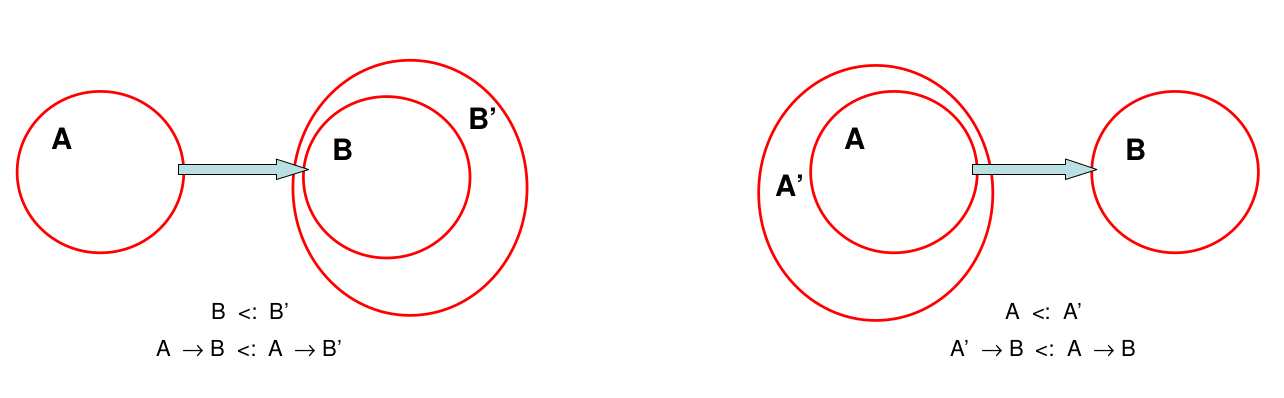
\includegraphics[scale=0.25]{img/subtipado/funciones-diagrama-perla.png}
    \caption{Esquema de Perla para entender el subtipado de funciones}
\end{figure}


\[
    \deriv{S-Arrow | S-Func}
        {\subt{\sigma'}{\sigma} \quad \subt{\tau}{\tau'}}
        {\subt
            {\tfunc{\sigma}{\tau}}
            {\tfunc{\sigma'}{\tau'}}
        }
\]

Para reemplazar una función por otra, tiene que
\begin{itemize}
    \item Bancarse todos los argumentos, o más (contravarianza)
    \item El resultado tiene que ser reemplazable (covarianza)
\end{itemize}

Se dice que el constructor de tipos de función es \textbf{contravariante} en el
primer argumento (dominio) y \textbf{variante} en el segundo (imagen).

\subsection{Subtipado de referencias}

Ref es \textbf{invariante}, solo se comparan referencias de tipos equivalentes

\[
    \deriv{S-Ref}
        {\subt{\sigma}{\tau} \quad \subt{\tau}{\sigma}}
        {\subt{\tref{\sigma}}{\tref{\tau}}}
\]

\textit{no hace falta que sean iguales, como con los registros y las permutaciones}.

\begin{nota}
    Justificación

    \textbf{Es ref covariante?}

    \[
        \deriv{S-Ref}
            {\subt{\sigma}{\tau}}
            {\subt{\tref{\sigma}}{\tref{\tau}}}
    \]

    Si tengo $r: \tref{Nat}$ y hago $\dealloc{r}$, que le puedo pasar? Y la
    escritura?

    Si fuera covariante, uno esperaría que como $\subt{Int}{Float}$,
    $\subt{\tref{Int}}{\tref{Float}}$. Pero si tengo

    \begin{verbatim}
    let r = ref 3  // r : Ref Int
    in
        r := 2.1;  // Ref Int <: Ref Float, T-Sub, r: Ref Float
        !r
        // r: Int
        // Pero 2.1 no es int!
    \end{verbatim}

    se rompe con la asignación.

    (el 2 es un int que lo puedo ver como 2.0, float, pero el 2.1 es un float y
    no lo puedo ver como int)

    \textbf{Es ref contravariante?}

    \[
        \deriv{S-Ref}
            {\subt{\sigma}{\tau}}
            {\subt{\tref{\tau}}{\tref{\sigma}}}
    \]

    Como $\subt{Int}{Float}$ y suponemos ref contravariante,
    $\subt{\tref{Float}}{\tref{Int}}$

    \begin{verbatim}
    let r = ref 2.1 // r: Ref Float
    in
        !r
        // Por Ref Float <: Ref Int y T-Sub, r: Ref Int
        // r: Int
        // Pero 2.1 no es Int!
    \end{verbatim}
\end{nota}

\subsubsection{Refinado de Ref}

Para permitir algún tipo de subtipado, se agregan nuevas clases referencias de
solo lectura y solo escritura. $\tsource{\sigma}$ de lectura y $\tsink{\sigma}$
de escritura.

\[
    \ederiv
        {\GStipa{M}{\tsource{\sigma}}}
        {\GStipa{\dealloc{M}}{\sigma}}
    \quad
    \ederiv
        {\GStipa{M}{\tsink{\sigma}} \quad \GStipa{N}{\sigma}}
        {\GStipa{\assign{M}{N}}{\tunit}}
\]

\begin{itemize}
    \item Source (lectura) es covariante
    
    \[
        \deriv{S-Source}
            {\subt{\sigma}{\tau}}
            {\subt{\tsource{\sigma}}{\tsource{\tau}}}
        \quad
        \ederiv
            {\subt{Int}{Float}}
            {\subt{\tsource{Int}}{\tsource{Float}}}
    \]

    $\dealloc{r}$ puede verse como $Float$ aunque $r$ sea de tipo
    $\tsource{Int}$.

    Si tengo un ref 3 y lo desreferencio, puedo verlo como int o float 3.0
    
    \begin{verbatim}
        let r = ref 3
        in
            !r  // por Source Int <: Source Float
        :: Float
    \end{verbatim}

    Si espero leer una ref a T, puedo esperar una ref a un tipo más bajo, más
    informativo.

    \item Sink (escritura) es contravariante.

    \[
        \deriv{S-Sink}
            {\subt{\tau}{\sigma}}
            {\subt{\tsource{\sigma}}{\tsource{\tau}}}
        \quad
        \ederiv
            {\subt{Int}{Float}}
            {\subt{\tsink{Float}}{\tsink{Int}}}
    \]

    Por ejemplo,

    \begin{verbatim}
        let r = ref 2.1
        in
            r := 3; // Usando Sink Float <: Sink Int
            !r
        :: Float
    \end{verbatim}

    Puedo coercionar 3 a 3.0 y no se rompe nada.

    Si espero escribir sobre una Ref a T, puedo esperar una Ref a un tipo más
    alto, menos informativo.
\end{itemize}

Se pueden relacionar con Ref,

\[
    \deriv{S-RefSource}
        {}
        {\subt{\tref{\tau}}{\tsource{\tau}}}
    \quad
    \deriv{S-RefSink}
        {}
        {\subt{\tref{\tau}}{\tsink{\tau}}}
\]

\subsection{Algoritmo}

Muy lindo todo, pero como lo usamos para tipar? Hasta ahora nuestras reglas eran
dirigidas por sintaxis, por lo que es inmediato implementar un algoritmo de
chequeo de tipos a partir de ellas.

Pero con T-Subs, está guiada por la \textit{oportunidad del tipo}, la podés
aplicar cuando quieras como convenga. Esto hace que \textbf{no sea evidente como
implementar un algoritmo} de chequeo de tipos a partir de las reglas, que no sea
determinístico. Nos podemos sacar de encima el problema?

Propuesta N°1 de sistema: cambio en la regla de aplicación

La única regla en la que realmente hace falta subtipar es en la
aplicación. Definimos una variante del sistema de tipado dirigida por sintaxis y
la notamos con $\mapsto$.

\newcommand{\GtipaAlt}[2]{\Gamma \mapsto #1 : #2}

\[
    \deriv{T-App}   
        {
            \GtipaAlt{M}{\tfunc{\select{\sigma}}{\tau}}
            \quad \GtipaAlt{N}{\select{\rho}}
            \quad \select{\subt{\rho}{\sigma}}
        }
        {\GtipaAlt{\app{M}{N}}{\tau}}
\]

(y cambiando el resto del sistema para que use el tipado alternativo $\mapsto$)

\begin{proposition} Se puede probar por inducción en las reglas de tipado que
    \begin{enumerate}
        \item $\GtipaAlt{M}{\sigma}$ implica que $\Gtipa{M}{\sigma}$
        \item $\Gtipa{M}{\sigma}$ implica que existe $\tau$ tal que
        $\GtipaAlt{M}{\tau}$ con $\subt{\tau}{\sigma}$.
    \end{enumerate}
\end{proposition}

Pero nos falta cubrir como implementar la relación $<:$. (recordar
\fullref{sec:subt-reglas} y S-Rcd). Las reglas S-Refl y S-Trans no están guiadas
por la sintaxis. Para sacarlas,

\begin{nota}
    Diego: Lo que sigue ahora es algo anecdótico
\end{nota}

\begin{itemize}
    \item S-Refl está para resolver cosas de la pinta $\subt{Nat}{Nat}$,
    entonces podemos remover la necesidad de la reflexividad agregando axiomas
    para cada tipo: $\subt{Nat}{Nat}$, $\subt{Float}{Float}$,
    $\subt{Bool}{Bool}$.

    \textit{Esto se puede probar en general pero no lo probamos}

    \item Con un argumento similar, se puede demostrar que no es necesaria
    S-Trans agregando todas las combinaciones.
\end{itemize}

Sacando esas dos reglas, la parte de subtipado puede ser guiada por sintaxis?
Si, el algoritmo es el siguiente

\begin{verbatim}
subtype(S, T) {
    // Si es un axioma, sabemos que si. Sino,
    // func
    if S == S1 -> S2 and T == T1 -> T2:
        return subtype(T1, S2) and subtype(S2, T2)
    
    // reg
    if S == {kj: Sj, j in 1..m} and T == {li: Ti, i in 1..n}:
        return {li, i in 1..n} subseteq {kj, j in 1..m} and
            forall i exists j kj = li and subtype(Sj, Ti)

    return false
}
\end{verbatim}

\chapter{Paradigma de objetos}

El modelo de cómputo que está detrás de POO, también puede caer diseño orientado
a objetos pero es mucho más complejo. Acá vamos a modelar una parte chiquita.

\section{Programación Orientada a Objetos}

\subsubsection{Conceptos y metáfora}

\begin{itemize}
    \item Todo programa es una simulación, y cada entidad del sistema siendo
    simulado se representa en el programa a través de un \textbf{objeto}
    \item Los objetos son la forma de abstraer un concepto físico o conceptual
    del mundo real
    \item El modelo de cómputo consiste en envío de mensajes: un sistema está
    formado por objetos que \textit{colaboran} entre sí mediante mensajes.
    \item Los \textbf{mensajes} son solicitudes para que un objeto lleve a cabo
    operación. El \textbf{receptor} (el objeto que lo recibe) decide como
    llevarla a cabo, cuya implementación está descripta por un \textbf{método}.
    \item El conjunto de mensajes que responde un objeto se denomina
    \textbf{interfaz} o \textbf{protocolo}.
    \item Los objetos pueden tener \textbf{estado} interno que altere el
    comportamiento de los métodos. Se representa a través de un conjunto de
    \textbf{colaboradores internos} (también llamados \textbf{atributos} o
    \textbf{variables instancia})
\end{itemize}

Ejemplo:

\begin{verbatim}
unRectangulo
    interfaz: area
    atributos: alto y ancho
    método: area = function() { return alto * ancho }
\end{verbatim}

La única manera de interactuar con un objeto es a través de su protocolo. Su
implementación no puede depender de detalles de implementación de otros objetos
(principio heredado de TADs)

\begin{definition*}[Principio de ocultamiento de la información]
    El estado de un objeto es \textbf{privado} y solamente puede ser consultado
    o modificado por sus métodos. \textit{(No todos los lenguajes imponen esta
    restricción)}
\end{definition*}

\subsection{Method dispatch}

Cómo hacemos por atrás para saber qué método de un objeto ejecutar cuando le
llega un mensaje? El proceso que establece la asociación mensaje-método a
ejecutar se llama \textbf{method dispatch}.

Si se hace en tiempo de \textit{compilación} (se puede determinar a partir del
código fuente) es \textbf{method dispatch estático}. En cambio, si se hace en
runtime es \textbf{method dispatch dinámico.}

\subsection{Corrientes}

Quien es responsabile de conocer los métodos de los objetos? Hay dos
alternativas conocidas: \textbf{clasificación} y \textbf{prototipado}

\subsection{Clasificación}

Es la más mainstream. Las clases modelan \textbf{conceptos abstractos} del
dominio de problema. Definen el comportamiento y la forma de un conjunto de
objetos que instancian (sus \textbf{instancias}). Todo objeto es instancia de
alguna clase. Son templates que tienen métodos, atributos y después se usan para
instanciar objetos concretos.

Tienen

\begin{itemize}
    \item Nombre
    \item Definición de variables de instancia
    \item Métodos de instancia. Por cada uno nombre, parámetros y cuerpo.
\end{itemize}

\begin{figure}[H]
    \centering
    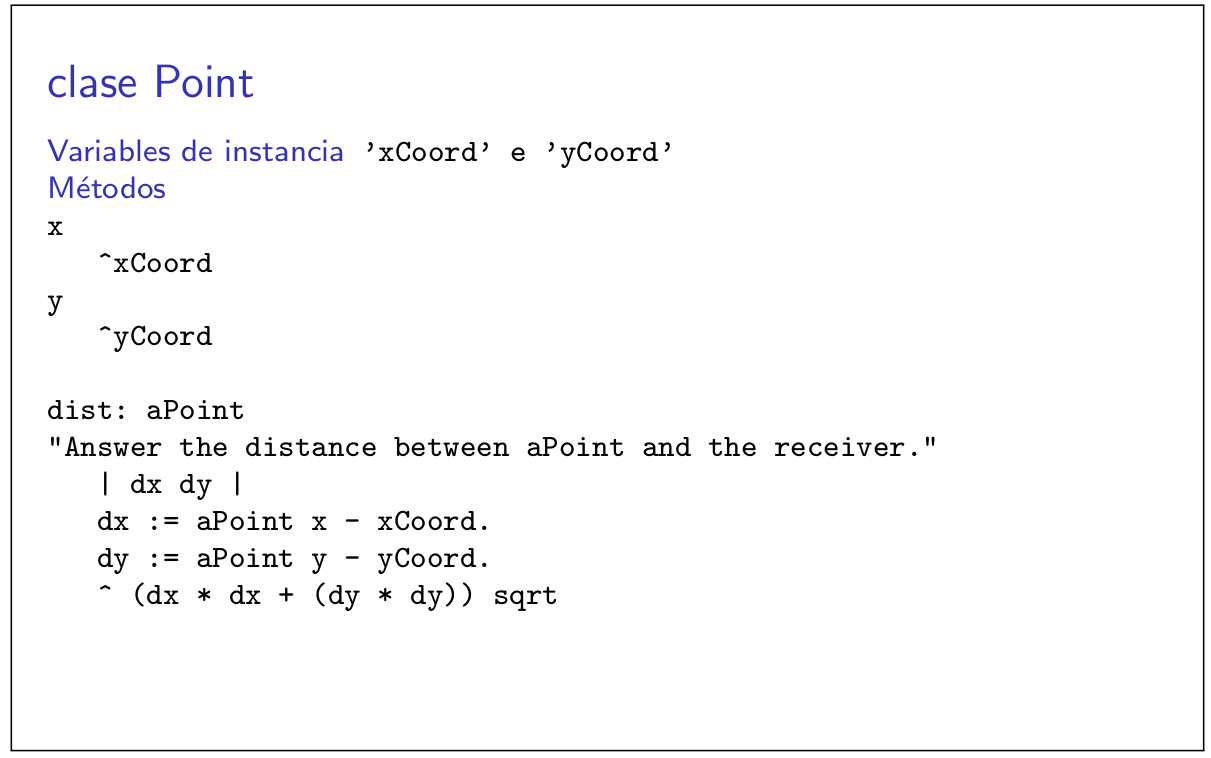
\includegraphics[scale=0.25]{img/poo/st-point.png}
    \caption{Ejemplo de clase en sintaxis de Smalltalk}
\end{figure}

\begin{figure}[H]
    \centering
    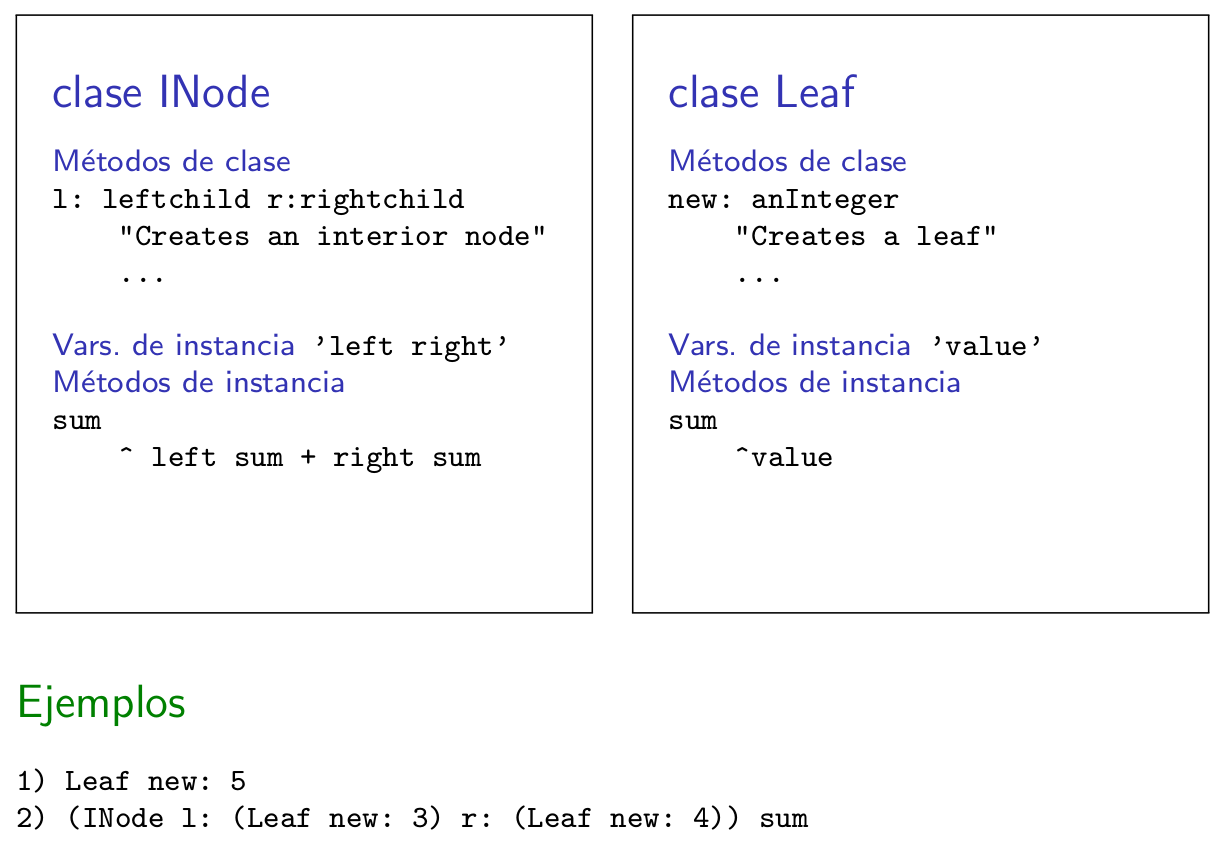
\includegraphics[scale=0.25]{img/poo/st-node.png}
    \caption{Ejemplo de clase Node en sintaxis de Smalltalk}
\end{figure}

\subsubsection{Self y super}

\textbf{self} es una pseudovariable que durante la ejecución de un
método referencia al receptor del mensaje. Se liga automáticamente y no puede
ser asignada.

\begin{figure}[H]
    \centering
    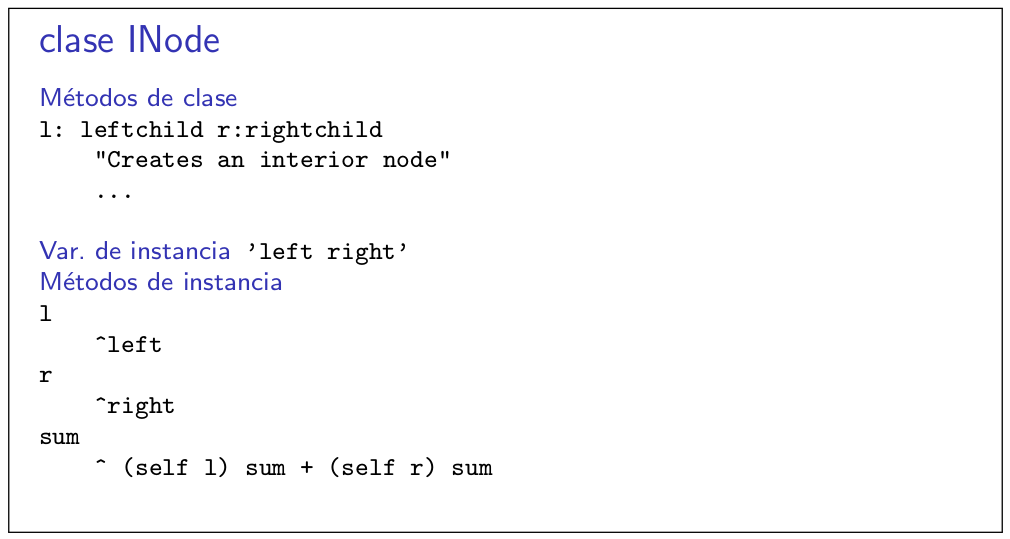
\includegraphics[scale=0.25]{img/poo/st-self.png}
    \caption{Ejemplo uso de self en Smalltalk}
\end{figure}

\textbf{super} es otra pseudovariable que referencia al objeto que recibe el
mensaje. Cambia el proceso de activación al momento del envío de un mensaje.

Una expresión de la forma \texttt{super msg} que aparece en el cuerpo de un
método \texttt{m} provoca que el \textbf{method lookup} se haga desde el padre
de la clase anfitriona de \texttt{m}.

\begin{figure}[H]
    \centering
    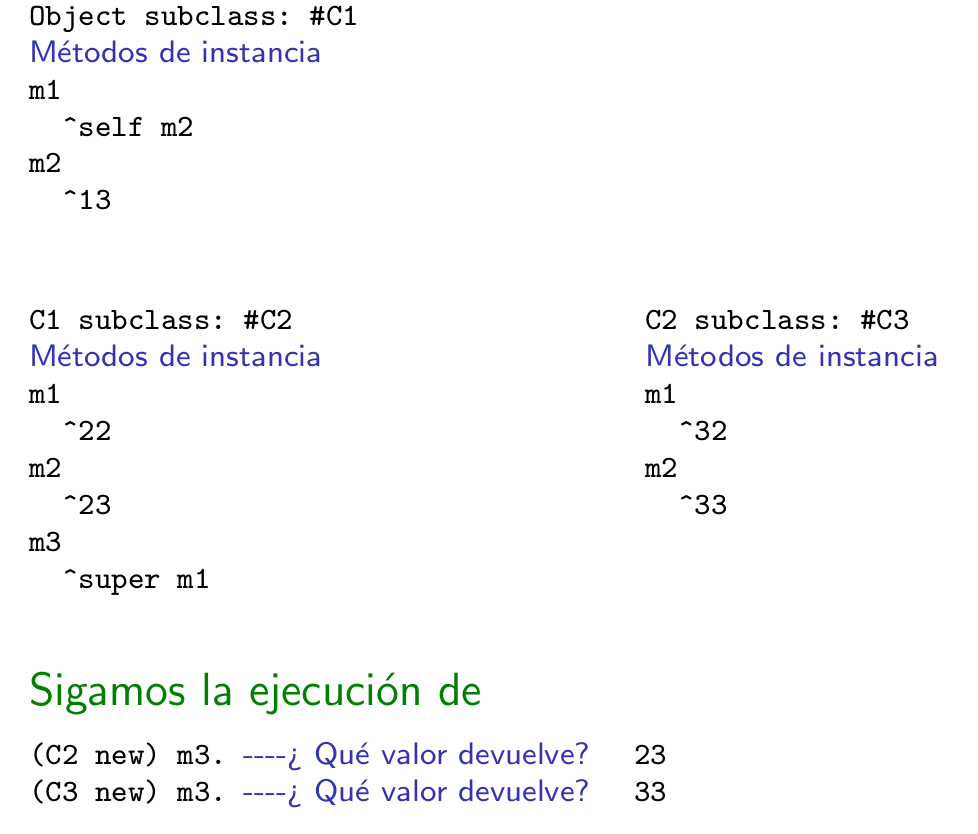
\includegraphics[scale=0.25]{img/poo/st-super-self.png}
    \caption{Ejemplo \texttt{super} y \texttt{self}}
\end{figure}

\subsubsection{Jerarquía de clases}

Es común que nuevas clases se definan como \textit{extensiones} de clases
existentes, agregando o cambiando el comportamiento de algunos métodos y
agregando nuevas variables de instancia o clase. Por eso, una clase puede
\textbf{heredar de} o \textbf{extender} de una clase existente (llamada
\textbf{superclase}). La transitividad de esta relación induce nociones de
\textbf{ancestros} y \textbf{descendientes}.

Hay dos tipos

\begin{itemize}
    \item \textbf{Simple}: una clase tiene un único padre (salvo la raíz). Esta
    es la que usan la mayoría de los lenguajes OO.
    \item \textbf{Múltiple}: una clase puede tener más de una clase padre.
    
    Complica el proceso de method dispatch, ya que si tengo un método $m$
    definido en más de una superclase, cual uso? Hay dos soluciones posibles:
    \begin{itemize}
        \item Establecer un \textit{orden de búsqueda} sobre las superclases
        \item Pedir que se \textit{redefinan} en la clase nueva todos los
        métodos que estén en más de una clase padre.
    \end{itemize}
    
\end{itemize}

\begin{figure}[H]
    \centering
    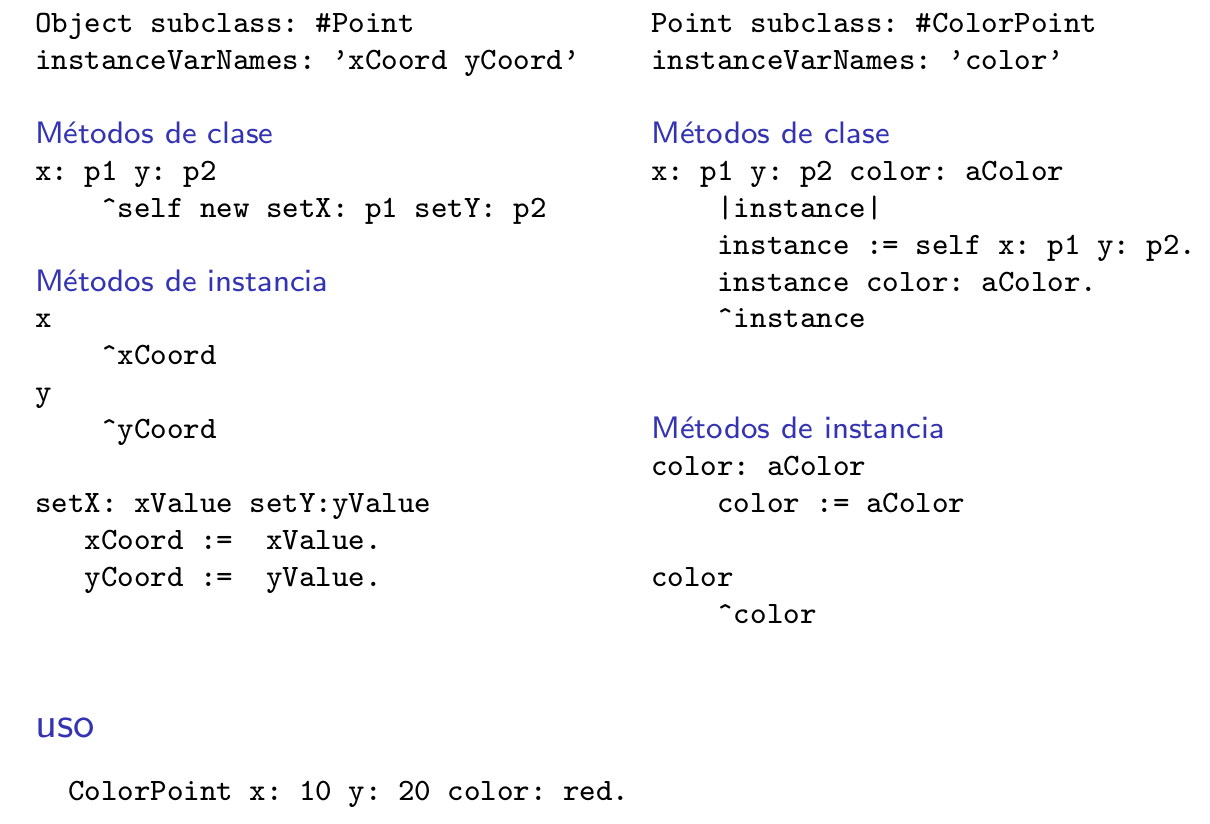
\includegraphics[scale=0.25]{img/poo/st-inheritance.png}
    \caption{Ejemplo de herencia en Smalltalk}
\end{figure}

\subsection{Prototipado}

Construye instancias concretas que se interpretan como representantes canónicos
de instancias (llamados prototipos). El resto de las instancias se generan
clonando los prototipos (de forma shallow). Y los clones se pueden cambiar.

Ejemplo de creado de objeto en js

\begin{minted}{javascript}
let celda = {
    contenido: 0,
    get: function() { return this.contenido; },
    set: function(n) { this.contenido = n; }
}

// Generar objetos
Celda = function() {
    this.contenido = 0;
    this.get = function() { return this.contenido; };
    this.set = function(n) { this.contenido = n; };
}

otracelda = new Celda();
\end{minted}

\newcommand{\obj}[1]{[\ #1\ ]} % objeto
\newcommand{\emptyobj}{[]} % objeto
\newcommand{\attr}[2]{#1 = #2} % atributo
\newcommand{\met}[2]{\varsigma (#1) #2} % method{args}{body}
\newcommand{\sel}[2]{#1.#2} % selección o envío de mensaje
\newcommand{\update}[3]{\sel{#1}{#2} \Leftarrow #3} % redefinición de método (update)
% TODO: Debería ser algún harpoon pero no encontré como hacerlo
\newcommand{\asgn}[3]{\sel{#1}{#2} := #3}

\newcommand{\sabs}[2]{\lambda(#1) #2} % sigma abs
\newcommand{\sapp}[2]{#1(#2)} % sigma app
\newcommand{\scall}[3]{\sel{#1}{\sapp{#2}{#3}}}

\newcommand{\sfv}[1]{\text{fv}(#1)}
\newcommand{\ssust}[3]{#1 \select{\{#2 / #3\}}} % sigma sust

\newcommand{\attrLi}{\attr{l_i}{\met{x_i}{\iesimo{b}}}}

\newcommand{\sderiv}[3]{\trfrac[{[}#1{]}]{#2}{#3}}
\newcommand{\bigreduces}{\longrightarrow}
\newcommand{\bigreduce}[2]{#1 \bigreduces #2}

\newcommand{\ubrace}[2]{\aunderbrace[l1r]{#1}_{#2}}
\newcommand{\obrace}[2]{\aoverbrace[L1R]{#1}^{#2}}

\section{Cálculo de objetos}

Acá vamos a hacer semántica big step en vez de small step. De un gran paso
llegás al valor. Vamos a ver un cálculo de objetos no tipado basado en Abadi y
Cardelli, 98 que se llama $\varsigma$ calculo (sigma pero una sigma cheta)

Ingredientes

\begin{itemize}
    \item Los objetos son la única estructura computacional
    \item Los objetos son registros que tienen métodos como atributos (un campo
    normal va a ser un método que devuelve siempre lo mismo)
    \item Cada método tiene una única variable ligada que representa a
    \texttt{self} (o \texttt{this}) y un cuerpo que produce el resultado, que
    puede depender o no de self.
    \item Proveen dos operaciones: envío de mensaje (invocar un método) o
    redefinición de un método.
\end{itemize}

\subsection{Sintaxis}

\begin{alignat*}{3}
    o, b ::=
    &  &&x  &&\text{\textit{variable}}\\
    &|\ &&\obj{\attr{l_i}{\met{x_i}{\iesimo{b}}}} 
    \quad&&\text{\textit{objeto}}\\
    &| &&\sel{o}{l} &&\text{\textit{selección / envío de mensaje}}\\
    &| &&\update{o}{l}{\met{x}{b}} &&\text{\textit{redefinición de método}}\\
\end{alignat*}

\begin{example*}
    \[
    o \eqdef \obj{
        \attr{l_1}{\met{x_1}{\obj{}}},\
        \attr{l_2}{\met{x_2}{\sel{x_2}{l_1}}}
    }
    \]

    \begin{itemize}
        \item $l_1$ retorna el objeto vacío
        \item $l_2$ envía el mensaje $l_1$ a self (representado por el parámetro $x_2$)
    \end{itemize}
\end{example*}

\subsection{Atributos vs métodos}

El cálculo $\varsigma$ no incluye explícitamente atributos (campos), sino que se
representan como métodos que no usan al parámetro self. De esta manera, el envío
de un mensaje representa también a la selección de un atributo y la redefinición
de un método representa también la asignación de un atributo

Como abusos de notación, vamos a

\begin{itemize}
    \item Usar $\obj{\dots, \attr{l}{b}, \dots}$ en vez de
    $\attr{l}{\met{x}{b}}$ cuando no se usa $x$ en $b$,
    \item Usar $\asgn{o}{l}{b}$ en vez de $\update{o}{l}{\met{x}{b}}$ cuando $x$
    no se usa en $b$.
\end{itemize}

\subsection{Variables libres}

$\varsigma$ es un ligador del parámetro self $x_i$ en el cuerpo $b_i$ de la
expresión $\met{x_i}{b_i}$.

\begin{nota}
    Esto es similar a lc, probablemente en semántica vamos a tener que hacer una
    sustitución para ligarla.
\end{nota}

\begin{definition}[Variables libres]
\begin{alignat*}{2}
    &\sfv{\met{x}{b}} &&= \sfv{b} \setminus \{ x \}\\
    &\sfv{x} &&= \{ x \} \\
    &\sfv{\obj{\attrLi}}
        &&= \bigcup_{i\in 1..n} \sfv{\met{x_i}{b_i}}\\
    &\sfv{\sel{o}{l}} &&= \sfv{o} \\
    &\sfv{\update{o}{l}{\met{x}{b}}} &&= \sfv{o.l} \cup \sfv{\met{x}{b}}
\end{alignat*}

Un término $o$ es \textbf{cerrado} si $\sfv{o} = \emptyset$.
\end{definition}

\subsection{Sustitución}

\begin{alignat*}{2}
    &\ssust{x}{c}{x} &&= c \\
    &\ssust{y}{c}{x} &&= y \\
    &\ssust{(\obj{\attrLi})}{c}{x}
    &&= \obj{
        \attr
            {l_i}
            {\ssust{(\met{x_i}{b_i})}{c}{x}^{i\in 1..n}}
    }\\
    &\ssust{(\sel{o}{l})}{c}{x} &&= \sel{\ssust{o}{x}{x}}{l}\\
    &\ssust{\update{o}{l}{\met{y}{b}}}{c}{x}
        &&= \update{(\ssust{o}{c}{x})}{l}{(\ssust{(\met{y}{b})}{c}{x})}\\
    &\ssust{(\met{y}{b})}{c}{x} &&=
        \met{y'}{\ssust{\ssust{b}{y'}{y}}{c}{x}}\\
    & && \qquad \text{con } y' \notin
        \sfv{\met{y}{b}}
        \cup \sfv{c}
        \cup \{ x \}
\end{alignat*}

Acomodamos las cosas para que no haya interferencias en la sustitución como
clashing de nombres (primer reemplazo) y una vez que tengamos eso, aplicamos la
sustitución que queremos.

\subsection{Equivalencia de términos ($\equiv$)}

Los términos $\met{x}{b}$ y $\met{y}{(\ssust{b}{y}{x})}$ con $y \notin
\sfv{b}$ se consideran equivalentes ($\alpha$-conversión).

También, dos objetos que difieren en el orden de sus componentes son
considerados equivalentes.

\[
    \obj{
        \attr{l_1}{\met{x_1}{\obj{}}},\
        \attr{l_2}{\met{x_2}{\sel{x_2}{l_1}}}
    }
    \equiv
    \obj{
        \attr{l_2}{\met{x_3}{\sel{x_3}{l_1}}},\
        \attr{l_1}{\met{x_1}{\obj{}}}
    }
\]

\subsection{Semántica operacional}

\begin{nota}
    En lc, las reducciones llevaban de $\reduce{M}{M'}$ y eventualmente
    aplicando muchas reducciones llegábamos a un valor. Acá vamos a llegar en
    una sola.
\end{nota}

Los valores van a ser objetos

\[
    v ::= \obj{\attrLi}
\]

Y vamos a aplicar reducciones \textbf{big-step} $\bigreduces$, que en un paso de reducción
pasan de una expresión a un valor.
\begin{gather*}
    \sderiv{Obj}{}{\bigreduce{v}{v}}\\\\
    \sderiv{Sel}
        {
            \bigreduce{o}{v'}
            \quad v' \equiv \obj{\attrLi}
            \quad \bigreduce{\ssust{b_j}{v'}{x_j}}{v}
            \quad j\in 1..n
        }
        {\bigreduce{\sel{o}{l_j}}{v}}\\\\
    \sderiv{Upd}
        {
            \bigreduce{o}{\obj{\attrLi}}
            \quad j \in 1..n
        }
        {
            \bigreduce
                {\update{o}{l_j}{\met{x}{b}}}
                {\obj{
                    \attr{l_j}{\met{x}{b}},\
                    \attr{l_i}{
                        \met{x_i}{b_i}^{i\in1..n-\{j\}}
                    }
                }}
        }
\end{gather*}

En Sel reduzco $o$ hasta un valor $v'$ para saber quien es self, ligo self en
$b_j$ que es el cuerpo del método correspondiente a $l_j$, y el resultado es
reducir eso a un valor

\begin{example*} Reducción de
\(
    o = \sel{
            \obj{
                \attr{a}{\emptyobj},\
                \attr{l}{\met{x}{\sel{x}{a}}}}
        }
        {l}
\)

\[
    \sderiv{Sel}
        {
            \sderiv{Obj}{}{\bigreduce{o}{o}}
            \qquad
            \sderiv{Sel}
                {
                    \sderiv{Obj}{}{\bigreduce{o}{o}}
                    \qquad
                    \sderiv{Obj}{}
                        {
                            \bigreduce
                                {
                                    \obrace{\ssust{\emptyobj}{o}{x}}{=\emptyobj}
                                }
                                {\emptyobj}
                        }
                }
                {
                    \bigreduce
                        {\obrace{\ssust{(\sel{x}{a})}{o}{x}}{=\sel{o}{a}}}
                        {\emptyobj}
                }
        }
        {
            \bigreduce
                {
                    \sel{
                        \ubrace{
                            \obj{
                                \attr{a}{\emptyobj},\
                                \attr{l}{\met{x}{\sel{x}{a}}}
                            }
                        }{o}
                    }
                    {l}
                }
                {\emptyobj}
        }
\]
\end{example*}

\begin{example*} Reducción de
\(
    \sel
    {
        (\update
            {
                \obj{
                    \attr{a}{\emptyobj},\
                    \attr{l}{\met{x}{\sel{x}{a}}}}
            }
            {l}
            {\met{y}{\emptyobj}})
    }
    {l}
\)

\[
    \sderiv{Sel}
        {
            \sderiv{Upd}
                {\sderiv{Obj}{}{\bigreduce{o}{o}}}
                {
                    \bigreduce{u}
                    {
                        \obj{
                            \attr{a}{\emptyobj},\
                            \attr{l}{\emptyobj}
                        }
                    }
                }
            \qquad
            \sderiv{Obj}{}
                {
                    \bigreduce
                    {
                        \obrace{\ssust{\emptyobj}{u}{x}}{=\emptyobj}
                    }
                    {\emptyobj}
                }
        }
        {
            \bigreduce
            {
                \ubrace{\sel
                {
                    (\update
                        {
                            \ubrace{
                                \obj{
                                    \attr{a}{\emptyobj},\
                                    \attr{l}{\met{x}{\sel{x}{a}}}}
                            }{o}
                        }
                        {l}
                        {\met{y}{\emptyobj}})
                }
                {l}}{u}
            }
            {\emptyobj}
        }
\]
\end{example*}

\begin{example*}
Podemos tener problemas, por ej. el siguiente tiene una reducción infinita
\(
    \sel{
        \ubrace{
        \obj{
            \attr{a}{\met{x}{\sel{x}{a}}}
        }
        }{o}
    }
    {a}
\)

es como una llamada recursiva, pero sin caso base. La evaluación de esta
expresión se indefine. Es análogo a $\fix{\abs{x}{\sigma}{x}}$.

\[
    \sderiv{Sel}
        {
            \sderiv{Obj}{}{\bigreduce{o}{o}}
            \qquad
            \sderiv{Sel}{\vdots}{
                \bigreduce
                {\obrace{\ssust{\sel{x}{a}}{o}{x}}{=\ \changed{\sel{o}{a}}}}
                {}
            }
        }
        {\bigreduce{\sel{o}{a}}{}}
\]

\end{example*}

\newcommand{\oname}[1]{\text{\texttt{#1}}}
\newcommand{\true}{\oname{true}}
\newcommand{\false}{\oname{false}}

\subsection{Ejemplo: Naturales}

Vamos a asumir que existen los objetos $\true$ y $\false$ que corresponden a
booleanos.

\begin{nota}
    Se podrían definir estilo Smalltalk, y tener métodos \texttt{ifTrue} e
    \texttt{ifFalse} que según el objeto ejecuten lo que le pasás o no.
\end{nota}

\begin{align*}
    \oname{zero} \eqdef \obj{
        &\attr{iszero}{\true},\\
        &\attr{pred}{\met{x}{x}},\\
        &\attr{succ}{
            \met{x}
            {
                \assign
                {
                    \sel
                    {
                        (\assign{\sel{x}{iszero}}{\false})
                    }
                    {pred}
                }
                {x}    
            }
        }
    }\\
    \oname{uno} \eqdef\ &\sel{\oname{zero}}{succ}\\
    \quad &
    \textcolor{gray}
    {
        \bigreduce{}
        {
            \ubrace{
                \obj{
                    \attr{iszero}{\false},
                    \attr{pred}{\oname{zero}},
                    \attr{succ}{\dots}
                }
            }{\oname{uno}'}
        }
    }\\
    \oname{dos} \eqdef\ &\sel{\oname{zero}}{\sel{succ}{succ}}\\
    \quad &
    \textcolor{gray}
    {
        \bigreduce{}
        {
            \obj{
                \attr{iszero}{\false},
                \attr{pred}{\oname{uno}'},
                \attr{succ}{\dots}
            }
        }
    }
\end{align*}

\subsection{Codificando calculo $\lambda$}

\newcommand{\cod}[1]{\llbracket #1 \rrbracket } % codificación del lambda cálculo

Podemos simular el cálculo $\lambda$ no tipado,

\[
    M ::= \app{M}{N} \mid \uabs{x}{M} \mid x
\]

\begin{nota}
    Queremos hacer esto porque los métodos del cálculo sigma no tienen
    argumentos, solo self. Idea intuitiva:

    \begin{itemize}
        \item Representar las funciones como objetos
        \[
            \obj{
                \attr{arg}{\dots},\
                \attr{val}{\dots}
            }.
        \]
        \item Al aplicarlas, primero se asigna el valor del argumento al
        atributo $arg$ y luego se envía el mensaje $val$ que evalúa el cuerpo de
        la función
        \item De esa forma, una evaluación (o aplicación) $(\app{f}{v})$ se
        traduce en
        \(
            \sel{(\assign{\sel{o_f}{arg}}{o_v})}{val}
        \)
    \end{itemize}

    Son esencialmente \textit{method objects} de ing1
\end{nota}

Vamos a definir una función $\cod{\cdot}: \tfunc{M}{a}$ que dado un término nos
da el objeto que lo codifica.
\begin{alignat*}{3}
    &\cod{x} &&\eqdef &&x\\
    &\cod{\app{M}{N}} &&\eqdef 
        &&\sel{(\assign{\sel{\cod{M}}{arg}}{\cod{N}})}{val}\\
    &\cod{\uabs{x}{M}} &&\eqdef
        \obj{
            &&\attr{val}{\ssust{\met{y}{\cod{M}}}{\sel{y}{arg}}{x}},\\
            & && &&\textcolor{gray}{\attr{arg}{\met{y}{\sel{y}{arg}}}}
        }
    \\ & && &&\text{con } y\notin \sfv{M}
\end{alignat*}

en $\uabs{x}{M}$ $M$ tiene apariciones libres de $x$, entonces las reemplazamos
por $\sel{y}{arg}$ para que funcione bien la semántica de la aplicación. En la
codificación de la función, $arg$ lo dejamos inicialmente como algo indefinido,
porque no tiene sentido que tenga nada real asignado ya que siempre lo vamos a
reemplazar.

Si hacemos $\sel{\cod{\uabs{x}{x}}}{val}$, se cuelga.

\begin{example}
Ejemplos de codificación

\begin{align*}
    \cod{\uabs{x}{x}} \eqdef\ &
        \obj{
            \attr{val}{\ssust{\met{y}{\cod{x}}}{\sel{y}{arg}}{x}},\
            \textcolor{gray}{\attr{arg}{\met{y}{\sel{y}{arg}}}}
        }\\
    =\ &\obj{
        \attr{val}{\ssust{\met{y}{x}}{\sel{y}{arg}}{x}},\
        \textcolor{gray}{\attr{arg}{\met{y}{\sel{y}{arg}}}}
    }\\
    =\ &\obj{
        \attr{val}{\met{y}{\sel{y}{arg}}},\
        \textcolor{gray}{\attr{arg}{\met{y}{\sel{y}{arg}}}}
    }
    \\\\
    \cod{\app{(\uabs{x}{x})}{M}} \eqdef\ &
    \sel
        {(\assign
            {\sel{\cod{\uabs{x}{x}}}{arg}}
            {\cod{M}}
        )}
        {val}\\
    =\ &\sel{
            \assign{
                \sel{
                    \obj{
                        \attr{val}{\met{y}{\sel{y}{arg}}},\
                        \textcolor{gray}{\attr{arg}{\met{y}{\sel{y}{arg}}}}
                    }
                }
                {arg}
            }
            {\cod{M}}
        }
        {val}\\
    &\bigreduces \cod{M}\\ &\text{ siempre que $\cod{M}$ sea un objeto}
\end{align*}
\end{example}

\subsubsection{Métodos con parámetros}

Usando este truquito de codificación podemos extender a nuestros métodos para
que reciban parámetros. Un método que espera un parámetro es un método cuya
definición codifica a una función

\[
    \met{y}{\cod{\uabs{x}{M}}}
\]

como notación, vamos a escribir

\begin{itemize}
    \item $\sabs{x}{M}$ en vez de $\cod{\uabs{x}{M}}$
    \item $\sapp{M}{N}$ en vez de $\cod{\app{M}{N}}$.
\end{itemize}

\subsubsection{Ejemplo: PUnto en el plano}

Lo definimos arrancando en el origen de coordenadas pero puede ser desplazado

\begin{align*}
    \oname{origen} \eqdef \obj{
        &\attr{x}{0},\\
        &\attr{y}{0},\\
        &\attr{mv\_x}{
            \met{p}{
                \sabs{d_x}{
                    \assign{\sel{p}{x}}{\sel{p}{x} + d_x}
                }
            }
        },\\
        &\attr{mv\_y}{
            \met{p}{
                \sabs{d_y}{
                    \assign{\sel{p}{y}}{\sel{p}{y} + d_y}
                }
            }
        }
    }
    \\
    \\
    \oname{unidad} \eqdef
        \sel{\oname{origen}}{\sel{\sapp{mv\_x}{1}}{\sapp{mv\_y}{1}}}
\end{align*}

\subsection{Codificación de clases}

\begin{nota}
    Partimos de una def de objetos que tenia métodos. Le dimos semántica,
    agregamos un encoding (no cambió la semántica) de parámetros, y ahora vamos
    a hacer otro encoding para \textbf{generadores de objetos} como los que
    vimos en prototipado pero ahora clases
\end{nota}

\subsubsection{(Stateless) Trait}

Un \textbf{trait} es una colección de ciertos métodos. Los stateless son un
conjunto particular de los traits que no tienen estado: no especifican variables
ni estado ni acceden al estado (i.e self). Una clase de construye a partir de
traits, a veces se usan para interfaces.

\begin{example}
    Ejemplo de trait

    \begin{alignat*}{1}
        \oname{CompT} \eqdef \obj{
            \attr{eq&}{
                \met{t}{\sabs{x}{\sabs{y}{
                    (\scall{x}{comp}{y}) == 0
                }}}
            },\\
            \attr{lt&}{
                \met{t}{\sabs{x}{\sabs{y}{
                    (\scall{x}{comp}{y}) < 0
                }}}
            }
        }
    \end{alignat*}

    Observar que en el cuerpo de los métodos $eq$ y $lt$, no se usa $t$ (self).
\end{example}

Los podemos pensar como una colección de \textbf{pre-métodos}: algo que
eventualmente será un método

\newcommand{\dtrait}{\oname{t} = \obj{
    \attr{l_i}{\sabs{y_i}{\iesimo{b}}}
}}

\begin{itemize}
    \item Un pre método es $\met{\select{t}}{\sabs{y}{b}}$ con $\select{t}
    \notin \sfv{\sabs{y}{b}}$ (i.e no usan self)
    \item En este caso por notación al ser un atributo podíamos omitir el
    $\met{t}{}$ y escribir directamente $\sabs{y}{b}$, por lo que los traits
    pasarían a ser

    \[ \dtrait \]
\end{itemize}

A partir de un trait $\dtrait$ podemos definir un constructor de objetos (cuando
$t$ es completo, tiene todos los métodos que necesita)

\[
    new \eqdef \sabs{\select{z}}{\obj{
        \attr{l_i}{\met{s}{
            \scall{\select{z}}{l_i}{s}^{i\in 1..n}
        }}
    }}
\]
\begin{align*}
    o &\eqdef \sapp{new}{\select{t}}\\
    &\approx \obj{
        \attr{l_i}{\met{s}{
            \scall{\select{t}}{l_i}{s}^{i\in 1..n}
        }}
    }\\
    &\approx \obj{
        \attr{l_i}{\met{y_i}{
            \iesimo{b}
        }}
    }\\
\end{align*}

$new$ aprovecha el trait para crear un método real (uno en el que el self
importa). Probablemente el $y_i$ sea lo que querramos usar después como self.

\begin{example*} Ejemplo de $new$
\begin{alignat*}{2}
    \oname{CompT} &\eqdef \obj{
        \attr{&&eq}{
            \met{t}{\sabs{x}{\sabs{y}{
                (\scall{x}{comp}{y}) == 0
            }}}
        },\\
        &\attr{&&lt}{
            \met{t}{\sabs{x}{\sabs{y}{
                (\scall{x}{comp}{y}) < 0
            }}}
        }
    }\\
    new &\eqdef &&\sabs{\select{z}}{\obj{
        \attr{l_i}{\met{s}{
            \scall{\select{z}}{l_i}{s}^{i\in 1..n}
        }}
    }}\\
    \sapp{new}{\oname{CompT}} &\approx
        \obj{
            \attr{&&eq}{\met{s}{\scall{\oname{CompT}}{eq}{s}}},\\
            & \attr{&&lt}{\met{s}{\scall{\oname{CompT}}{lt}{s}}}
        }\\
    &\approx
        \obj{
            \attr{&&eq}{
                \met{x}{\sabs{y}{
                    (\scall{x}{comp}{y}) == 0
                }}
            },\\
            & \attr{&&lt}{
                \met{x}{\sabs{y}{
                    (\scall{x}{comp}{y}) < 0
                }}
            }
        }
\end{alignat*}

Acá el objeto creado es inutilizable, porque \oname{CompT} usa $comp$ que no es
un método que define (no es completo).

\end{example*}

\subsubsection{Clases}

Una \textbf{clase} va a ser un \textit{trait} (completo) que además
provea un método $new$.

\begin{align*}
    \oname{c} \eqdef \obj{
        \attr{new&}{
            \sabs{\select{z}}{\obj{
                \attr{l_i}{\met{s}{
                    \scall{\select{z}}{l_i}{s}^{i\in 1..n}
                }}
            }}
        },\\
        \attr{l_i&}{
            \sabs{s}{\iesimo{b}}
        }
    }
\end{align*}

Luego,
\begin{align*}
    o &\eqdef \sel{\oname{c}}{new}\\
    &\bigreduces \obj{
        \attr{l_i}{\met{\green{s}}{\scall{c}{l_i}{\green{s}}^{i\in 1..n}}}
    }\\
    &\approx \obj{
        \attr{l_i}{\met{\green{s}}{\iesimo{b}}}
    }
\end{align*}

\begin{nota}
Observar que las clases son traits que \textbf{no} son \textit{stateless},
ya que $new$ tiene $z$ que hace referencia a self. Si no fuera así, para
instanciar una clase nueva habría que hacer $c.new(c)$ en vez de $c.new$, lo
cual no tiene mucho sentido.
\end{nota}

\begin{example*}
Clase Contador

\begin{align*}
    \oname{Contador} \eqdef \obj{
        \attr{new&}{
            \sabs{z}{[\
                \begin{aligned}[t]
                    \attr{v&}{\met{s}{\scall{z}{v}{s}}},\\
                    \attr{inc&}{\met{s}{\scall{z}{inc}{s}}},\\
                    \attr{get&}{\met{s}{\scall{z}{get}{s}}}\ ],
                \end{aligned}
            }
        }\\
        \attr{v&}{\sabs{s}{0}},\\
        \attr{inc&}{\sabs{s}{\assign{\sel{s}{v}}{\sel{s}{v} + 1}}},\\
        \attr{get&}{\sabs{s}{\sel{s}{v}}}
    }
\end{align*}
\end{example*}

\subsubsection{Herencia}

Si tenemos una clase

\begin{align*}
    \oname{c} \eqdef \obj{
        \attr{new&}{
            \sabs{\select{z}}{\obj{
                \attr{l_i}{\met{s}{
                    \scall{\select{z}}{l_i}{s}^{i\in 1..n}
                }}
            }}
        },\\
        \attr{l_i&}{
            \sabs{s}{\iesimo{b}}
        }
    }
\end{align*}

Queremos definir $\oname{c}'$ como subclase de \oname{c} que agregue los
pre-métodos $\sabs{s}{b_k^{k\in n+1..n+m}}$. Alcanza con agregar los métodos
nuevos, y para los viejos referenciar a la superclase.

\begin{align*}
    \oname{c} \eqdef \obj{
        \attr{new&}{
            \sabs{\select{z}}{\obj{
                \attr{l_i}{\met{s}{
                    \scall{\select{z}}{l_i}{s}^{i\in 1..n\changed{+m}}
                }}
            }}
        },\\
        \attr{l_j&}{
            \sel{c}{l_j^{j\in 1..n}}
        },\\
        \attr{l_k&}{
            \sabs{s}{b_k^{k\in n+1..n+m}}
        }
    }
\end{align*}

también si quisiéramos podríamos redefinir pre-métodos. En vez de delegar a la
superclase, los definimos y ya.

%%%%%%%

% LP
%% sintaxis
\newcommand{\no}[1]{\neg #1}
\newcommand{\y}[2]{#1 \wedge #2}\
\newcommand{\por}[2]{#1 \vee #2}
\newcommand{\impl}[2]{#1 \supset #2}
\newcommand{\sii}[2]{#1 \iff #2}

\newcommand{\propVars}{\mathcal{V}}

%% semántica
\newcommand{\sat}[2]{#1 \models #2}
\newcommand{\nsat}[2]{#1 \not\models #2}

%% resolución
\newcommand{\set}[1]{\{ #1 \}} % para fnc
\newcommand{\emptyCl}{\square} % clausula vacía
\newcommand{\opuesto}[1]{\overline{#1}}
\newcommand{\resol}[2]{\trfrac{#1}{#2}}

% LPO
\newcommand{\LPO}{\mathcal{L}}
\newcommand{\paratodo}[2]{\forall #1 . #2}
\newcommand{\existe}[2]{\exists #1 . #2}

\newcommand{\lpoass}[3]{#1[#2 \gets #3]}
\newcommand{\posat}[1]{s \models_M #1}
\newcommand{\notposat}[1]{s \not\models_M #1}

\newcommand{\sk}[1]{\text{\textbf{SK}}(#1)} % skolemizacion

%% resolución
\newcommand{\sust}[2]{#1 \gets #2}

\chapter{Paradigma lógico}

\begin{nota}
    Hasta ahora, vimos

    \begin{itemize}
        \item \textbf{Imperativo}: tenemos un estado compuesto por variables que
        se va modificando con las instrucciones, al final determinando un estado
        final.
        \item \textbf{Funcional}: tenemos expresiones que se van reduciendo
        hasta una forma que si todo sale bien es un valor
        \item \textbf{Objetos}: objetos como una forma de modelar la realidad,
        que colaboran mediante mensajes. Los métodos se implementan de forma
        imperativa, pero no es lo fundamental del paradigma. Eso es la
        colaboración mediante mensajes.
    \end{itemize}
\end{nota}

Se basa en el uso de la lógica como forma de programar. En vez de pensar en un
algoritmo dado un problema, nos mantenemos en la misma "esfera". En vez de
programar un problema, quedarnos en el \textit{qué}.

Vamos a especificar \textbf{hechos} y \textbf{reglas de inferencia} y un
\textbf{goal} (objetivo) a probar. Un motor de inferencia trata de probar que el
goal es consecuencia de los hechos y reglas.

Es \textbf{declarativo}: se especifican hechos, reglas y goals sin indicar
\textit{cómo} se obtiene el último a partir de los primeros.

Vamos a usar \textbf{Prolog}:

\begin{itemize}
    \item Los programas se escriben en un subconjunto de la logica de primer
    orden (cláusulas de Horn)
    \item El mecanismo teórico en el que se basa es el \textbf{método de
    resolución} (forma de dada una fórmula ver si es SAT o UNSAT)
    \item Para motivarlo, primero vamos a ver como es resolución en lógica
    proposicional
\end{itemize}

\section{Resolución para Lógica Proposicional}

\subsection{Lógica proposicional}

\subsubsection{Sintaxis}

Dado un conjunto $\propVars$ de \textbf{variables proposicionales}, podemos
definir inductivamente al conjunto de \textbf{fórmulas proposicionales} (o
\textbf{proposiciones}) \textbf{Prop} de la siguiente manera,

\begin{enumerate}
    \item Una variable proposicional $P_0, P_1, \dots$ es una proposición
    \item Si A, B son proposiciones, entonces también lo son
    \begin{itemize}
        \item $\no{A}$ (negación)
        \item $\y{A}{B}$ (conjunción)
        \item $\por{A}{B}$ (disyunción)
        \item $\impl{A}{B}$ (implicación)
        \item $\sii{A}{B}$
    \end{itemize}

\end{enumerate}
\begin{example*}
    Ejemplos de fórmulas: 
    $\por{A}{\no{B}}, \impl{\y{A}{B}}{\por{A}{B}}$
\end{example*}

\subsubsection{Semántica}

Una \textbf{valuación} es una función $v: \tfunc{\propVars}{\{ T, F \}}$ que
asigna valores de verdad a las variables proposicionales. \textbf{Satisface} una
proposición $A$ si $\sat{v}{A}$ donde,

\begin{alignat*}{2}
    \sat{v}{P} & \text{ sii } && v(P) = T\\
    \sat{v}{\no{A}} & \text{ sii }&& \nsat{v}{A} \text{ (i.e no $\sat{v}{A}$)}\\
    \sat{v}{\por{A}{B}} & \text{ sii }&& \sat{v}{A} \text{ o } \sat{v}{B}\\
    \sat{v}{\y{A}{B}} & \text{ sii }&& \sat{v}{A} \text{ y } \sat{v}{B}\\
    \sat{v}{\impl{A}{B}} &\text{ sii }&& \nsat{v}{A} \text{ o } \sat{v}{B}\\
    \sat{v}{\sii{A}{B}} & \text{ sii }&& (\sat{v}{A} \text{ sii } \sat{v}{B})
\end{alignat*}

\subsubsection{Tautologías y satisfacibilidad}

Una proposición $A$ es

\begin{itemize}
    \item una \textbf{tautología} si $\sat{v}{A}$ para toda valuación $v$ 
    (ej: $\por{P}{\no{P}}$)
    \item \textbf{satisfacible} si existe una valuación $v$ tal que $\sat{v}{A}$
    \item \textbf{insatisfacible} si no es satisfacible
\end{itemize}

Se puede extender a un conjunto. Un conjunto de proposiciones $S$ es 

\begin{itemize}
    \item \textbf{satisfacible} si existe una valuación $v$ tal que para todo $A
    \in S$, $\sat{v}{A}$. (otra forma de verlo: hace verdadera a la conjunción
    de todas)
    \item \textbf{insatisfacible} si no es satisfacible
\end{itemize}

\begin{example*}
    Ejemplos de tautologías
    \begin{itemize}
        \item $\impl{A}{A}$
        \item $\impl{\no{\no{A}}}{A}$
        \item $\sii{(\impl{A}{B})}{(\impl{\no{B}}{\no{A}})}$ (contrarecíproco)
    \end{itemize}
    
\end{example*}

\begin{example*} Ejemplos de proposiciones insatisfacible
    \begin{itemize}
        \item $\y{(\por{\no{A}}{B})}{\y{(\por{\no{A}}{\no{B}})}{A}}$
        \item \(
            \y
                {(\impl{A}{B})}
                {\y
                {A}
                {\no{B}}
                }
        \)
    \end{itemize}
\end{example*}

\begin{nota}
    Una forma de probar tautologías es con una tabla de verdad. Sin importar los
    valores de las variables proposicionales, tiene que dar verdadero. Para
    probar que algo es insat, lo mismo pero viendo que todo da falso.
\end{nota}

\begin{theorem}\label{teo:taut-sii-insat}
    Una proposición $A$ es una tautología sii $\no{A}$ es insatisfacible.
\end{theorem}
\begin{proof}[Dem.] Por la ida y la vuelta
    \begin{itemize}
        \item[$\Rightarrow$)] Si $A$ es taut. para toda valuación $v$,
        $\sat{v}{A}$. Entonces $\nsat{v}{\no{A}}$.
        \item[$\Leftarrow$)] Si $\no{A}$ es insatisfacible, para toda valuación
        $v$ $\nsat{v}{\no{A}}$. Luego $\sat{v}{A}$.
    \end{itemize}
\end{proof}

\begin{nota}
Esto sugiere un método indirecto para probar que una prop $A$ es una
tautología, probando que $\no{A}$ es insatisfacible.

Suele ser más fácil refutar que probar. Entonces si queremos probar $P$,
refutamos $\no{P}$. Esto entonces va a ser útil porque a los mecanismos de
resolución les va a ser más fácil refutar.
\end{nota}

\subsection{Resolución}

\begin{definition*}[Principio de demostracion por \textbf{refutación}]
    Vamos a probar que A es \textbf{válido} mostrando que $\no{A}$ es \textbf{insatisfacible}.
\end{definition*}

Hay varias técnicas de demostración por refutación

\begin{itemize}
    \item Tableaux semántico (1960)
    \item Procedimiento de Davis-Putnam (1960)
    \item \textbf{Resolución} (1965) (nos vamos a enfocar en este)
\end{itemize}

El método de resolución fue introducido por Alan Robinson en 1965, es simple de
implementar, y se usa mucho en el ámbito de demostración automática de teoremas.
Tiene una única regla de inferencia: \textbf{regla de resolución}. Y si bien no
es imprescindible, por conveniencia vamos a asumir que las fórmulas están en
\textbf{forma normal conjuntiva} (FNC).

\subsubsection{Forma normal conjuntiva (FNC)}\label{sec:logico-prop-fnc}

Un \textbf{literal} es una variable proposicional $P$ o su negación $\no{P}$.
Una proposición $A$ está en \textbf{FNC} si es una conjunción

\[
    C_1 \wedge \dots \wedge C_n
\]

donde cada $C_i$ (llamado \textbf{cláusula}) es una disyunción

\[
    B_{i1} \vee \dots \vee B_{in_i}
\]

y cada $B_{ij}$ es un literal. Una FNC es entonces una ``conjunción de
disyunciones de literales''

\begin{example*}Ejemplos de FNC
    \begin{itemize}
        \item $\y{(\por{P}{Q})}{(\por{P}{\no{Q}})}$ está en FNC
        \item $\y{(\por{P}{Q})}{(\por{P}{\no{\no{Q}}})}$ no está en FNC que
        tiene un doble neg en $C_2$.
        \item $\por{(\y{P}{Q})}{P}$ no está en FNC.
    \end{itemize}
\end{example*}

\begin{theorem}
    Para toda proposición $A$ puede hallarse una proposición $A'$ en FNC que es
    lógicamente equivalente para $A$.
\end{theorem}

\begin{nota}
    Decimos que $A$ es lógicamente equivalente a $B$ sii $\sii{A}{B}$ es una
    tautología.
\end{nota}

\subsubsection{Notación conjuntista de FNC}

Tomando en cuenta que tanto el $\vee$ como $\wedge$,

\begin{itemize}
    \item son conmutativos ($\sii{(\por{A}{B})}{(\por{B}{A})}$)
    \item son asociativos
    ($\sii{(\por{(\por{A}{B})}{C})}{(\por{A}{(\por{B}{C})})}$)
    \item son idempotentes ($\sii{(\por{A}{A})}{A}$)
\end{itemize}

podemos asumir que 

\begin{itemize}
    \item Cada cláusula $C_i$ es \textbf{distinta} (si fueran iguales, por
    idempotencia las podría juntar).
    \item Cada cláusula puede verse como un conjunto de literales distintos.
\end{itemize}

Por lo tanto podemos notar una FNC como
\[
    \set{C_1, \dots, C_n}
\]
donde cada $C_i$ es un conjunto de literales
\[
    \set{B_{i1}, \dots, B_{in_i}}
\]

\begin{example*}
    La FNC $\y{(\por{P}{Q})}{(\por{P}{\no{Q}})}$ se nota como
    \[
        \set{
            \set{P, Q},
            \set{P, \no{Q}}
        }
    \]
\end{example*}

\subsubsection{Principio fundamental del método de resolución}\label{sec:logico-lpo-resol-ppio-fundamental}

La resolución se basa en el hecho de que la siguiente proposición es una
\textbf{tautología},

\[
    \sii
    {
        \y{(\por{A}{P})}{(\por{B}{\no{P}})}
    }
    {
        \y
        {(\por{A}{P})}
        {
            \y
            {(\por{B}{\no{P}})}
            {(\por{A}{B})}
        }
    }
\]

\textit{Intuitivamente, si vale $P$ entonces no puede valer $\no{P}$, por lo que
tiene que valer B valga o no A, y lo mismo al revés}

Por lo tanto, el conjunto de cláusulas
\[
    \set{
        C_1, \dots, C_m,
        \set{A, P},
        \set{B, \no{P}}
    }
\]
es \textbf{lógicamente equivalente} a
\[
    \set{
        C_1, \dots, C_m,
        \set{A, P},
        \set{B, \no{P}},
        \select{\set{A, B}}
    }
\]

y entonces el primero va a ser \textbf{insatisfacible} sii el segundo lo es.

La cláusula $\set{A, B}$ se llama \textbf{resolvente} de las cláusulas $\set{A,
P}$ y $\set{B, \no{P}}$.

El resolvente de las cláusulas $\set{P}$ y $\set{\no{P}}$ es la \textbf{cláusula
vacía} (porque es insatisfacible) y se anota $\emptyCl$. El vacío significa
\textit{falso}, como era un y de todo, podemos concluir que es insatisfacible.

\subsubsection{Regla de resolución}

\begin{definition*}[Opuesto]
    Dado un literal $L$, el \textbf{opuesto} de $L$ $\opuesto{L}$ se define como
    \begin{itemize}
        \item $\no{P}$ si $L = P$
        \item $P$ si $L = \no{P}$
    \end{itemize}

    \begin{nota}
        Tenemos que definir esto para poder devolver la negación de un literal
        sin agregarle símbolos.
    \end{nota}
\end{definition*}

\begin{definition*}[Resolvente]
    Dadas dos cláusulas $C_1, C_2$ una cláusula C se dice \textbf{resolvente de
    $\bm{C_1}$ y $\bm{C_2}$} sii para algún literal $L$, $L \in C_1, \opuesto{L}
    \in C_2$ y

    \[
        C = (C_1 - \set{L}) \cup (C_2 - \set{\opuesto{L}})
    \]

    \begin{nota}
        Esto es lo de antes pero escrito más formal.
    \end{nota}

    \begin{example*} Ejemplos
        \begin{itemize}
            \item Las cláusulas $\set{A, B}$ y $\set{\no{A}, \no{B}}$ tienen dos
            resolventes: $\set{A, \no{A}}$ y $\set{B, \no{B}}$.
            \item Las cláusulas $\set{P}$ y $\set{\no{P}}$ tienen a la cláusula
            vacía $\emptyCl$ como resolvente.
        \end{itemize}
    \end{example*}
\end{definition*}

\begin{definition*}[Regla de resolución]
    En base a lo anterior podemos definir la \textbf{regla de resolución} como
    sigue,
    \[
        \resol
        {
            \set{A_1, \dots, A_m, \select{Q}}
            \quad
            \set{B_1, \dots, B_n, \select{\no{Q}}}
        }
        {
            \changed{
                \set{A_1, \dots, A_m, B_1, \dots, B_n}
            }
        }
    \]
\end{definition*}
\begin{example*} El resultado de aplicar la regla de resolución a
    \[
        \set{
            \set{P, \select{Q}},
            \set{P, \select{\no{Q}}},
            \set{\no{P}, Q},
            \set{\no{P}, \no{Q}}
        }
    \]
    es
    \[
        \set{
            \set{P, Q},
            \set{P, \no{Q}},
            \set{\no{P}, Q},
            \set{\no{P}, \no{Q}},
            \changed{\set{P}}
        }
    \]
\end{example*}

\subsubsection{Método de resolución}

El proceso de agregar a un conjunto $S$ el resolvente $C$ de dos cláusulas $C_1,
C_2 \in S$ (aplicando la regla de resolución a S) se llama \textbf{paso de
resolución}. (asumimos $C \notin S$)

\begin{nota}
    Recordamos que los pasos de resolución preservan la insatisfacibilidad,
    \[
        S \text{ es insatisfacible}
        \iff
        S \cup \set{C} \text{ es insatisfacible}
    \]
    ya que eran lógicamente equivalentes, como vimos en \fullref{sec:logico-lpo-resol-ppio-fundamental}
\end{nota}

Vamos a aplicar el metodo para obtener una \textbf{refutación}. Un conjunto de
cláusulas se llama una refutación si contiene la cláusula vacía ($\emptyCl$).

De esa forma, el método de resolución trata de constuir una secuencia de
conjuntos de cláusulas obtenidas usando pasos de resolución hasta llegar a una
\textbf{refutación}
\[
    S_1 \Rightarrow S_2 \Rightarrow \dots S_{n-1} \Rightarrow S_n \ni \emptyCl
\]
en este caso, sabemos que el \textit{conjunto inicial} de cláusulas es
insatisfacible, dado que cada paso de resolución preserva la insatisfacibilidad
y el último conjunto de cláusulas es insatisfacible.

\subsubsection{Ejemplos}

\begin{example*}
    \(\set{
        \set{P, Q},
        \set{P, \no{Q}},
        \set{\no{P}, Q},
        \set{\no{P}, \no{Q}}
    }\) es insatisfacible.

    \begin{enumerate}
        \item \(\set{
            \select{\set{P, Q}},
            \select{\set{P, \no{Q}}},
            \set{\no{P}, Q},
            \set{\no{P}, \no{Q}}
        }\)
        \item \(\set{
            \set{P, Q},
            \set{P, \no{Q}},
            \select{\set{\no{P}, Q}},
            \select{\set{\no{P}, \no{Q}}},
            \set{P}
        }\)
        \item \(\set{
            \set{P, Q},
            \set{P, \no{Q}},
            \set{\no{P}, Q},
            \set{\no{P}, \no{Q}},
            \select{\set{P}},
            \select{\set{\no{P}}}
        }\)
        \item \(\set{
            \set{P, Q},
            \set{P, \no{Q}},
            \set{\no{P}, Q},
            \set{\no{P}, \no{Q}},
            \set{P},
            \set{\no{P}},
            \changed{\emptyCl}
        }\)
    \end{enumerate}
\end{example*}

\begin{example*}
\(\set{
    \set{A, B, \no{C}},
    \set{A, B, C},
    \set{A, \no{B}},
    \set{\no{A}}
}\) es insatisfacible
\begin{enumerate}
    \item \(\set{
        \select{\set{A, B, \no{C}}},
        \select{\set{A, B, C}},
        \set{A, \no{B}},
        \set{\no{A}}
    }\)
    \item \(\set{
        \set{A, B, \no{C}},
        \set{A, B, C},
        \select{\set{A, \no{B}}},
        \set{\no{A}},
        \select{\set{A, B}}
    }\)
    \item \(\set{
        \set{A, B, \no{C}},
        \set{A, B, C},
        \set{A, \no{B}},
        \select{\set{\no{A}}},
        \set{A, B},
        \select{\set{A}}
    }\)
    \item \(\set{
        \set{A, B, \no{C}},
        \set{A, B, C},
        \set{A, \no{B}},
        \set{\no{A}},
        \set{A, B},
        \set{A},
        \changed{\emptyCl}
    }\)
\end{enumerate}
\end{example*}

\subsubsection{Formulas satisfacibles}

Queremos mostrar que $S = \set{\set{A, B, C}, \set{A}, \set{B}}$ es
insatisfacible, pero no podemos aplicar ningún paso de resolución a $S$ porque
no hay negaciones. Por lo tanto, no puede llegarse a una refutación a partir de
$S$. En lógica proposicional, estamos seguros entonces que $S$ debe ser
satisfacible. Efectivamente, podemos tomar por ej.
$v(A) = v(B) = \text{\textbf{T}}$.

\subsubsection{Terminación}

La aplicación reiterada de la regla de resolución \textbf{siempre termina}
(suponiendo que el resolvente que se agrega es nuevo). Ya que,

\begin{enumerate}
    \item El resolvente (la cláusula nueva que se agrega) se forma con los
    literales distintos que aparecen en el conjunto de las cláusulas de partida
    $S$.
    \item Hay una cantidad \textbf{finita} de literales en el conjunto de
    cláusulas de partida $S$.
\end{enumerate}

En el peor de los casos, la regla de resolución podrá generar una nueva cláusula
por cada combinación diferente de literales distintos de $S$. Pero sigue siendo
finita y por lo tanto termina.

\subsubsection{Corrección y completitud}

\begin{theorem}
    Dado un conjunto finito $S$ de cláusulas, $S$ es insatisfacible sii tiene
    una refutación.
\end{theorem}

Este resultado establece la corrección y completitud del método de resolución.

\begin{nota}
    En LPO no es tan bueno. Si encuentra una refutación significa que es
    insatisfacible (correcto) pero puede pasar que no la encontremos
    (incompleto).
    \todo{Validar que esté bien el uso de correcto e incompleto}.
\end{nota}

\subsubsection{Resumen del algoritmo}

Para probar que $A$ es una tautología hacemos lo siguiente,

\begin{enumerate}
    \item Calculamos la FNC de $\no{A}$
    \item Aplicamos el método de resolución
    \item \select{Si hallamos una refutación}, entonces $\no{A}$ es
    insatisfacible y por lo tanto $A$ es una tautología. (Por Teo.
    \ref{teo:taut-sii-insat})
    \item \changed{Si no hallamos ninguna refutación}, entonces $\no{A}$ es
    satisfacible y por lo tanto $A$ no es una tautologia. (Por negación de Teo.
    \ref{teo:taut-sii-insat})
\end{enumerate}

\section{Lógica de Primer Orden}

\subsection{Sintaxis}

\begin{definition*}[Lenguaje de primer orden]
    Un lenguaje de primer orden (LPO) $\LPO$ consiste en
    \begin{enumerate}
        \item Un conjunto numerable de \textbf{constantes} $c_0, c_1, \dots$
        \item Un conjunto numerable de \textbf{símbolos de función} con aridad
        $n > 0$ (indicando el número de argumentos) $f_0, f_1, \dots$.
        \item Un conjunto numerable de \textbf{símbolos de predicado} con aridad
        $n \geq 0$, $P_0, P_1, \dots$. Si $n = 0$, es una variable
        proposicional.
    \end{enumerate}
\end{definition*}

\begin{definition*}[Término]
    Sea $\mathcal{V} = \set{x_0, x_1, \dots}$ un conjunto numerable de variables
    y $\LPO$ un LPO. El conjunto de \textbf{$\LPO$-términos}
    se define inductivamente como

    \begin{enumerate}
        \item Toda constante de $\LPO$ y toda variable es un $\LPO$-término.
        \item Si $t_1, \dots, t_n \in$ $\LPO$-términos y $f$ es un símbolo de
        función de aridad $n$, entonces $f(t_1, \dots, t_n) \in$ $\LPO$-términos
    \end{enumerate}
\end{definition*}

\begin{definition*}[Fórmulas atómicas]
    Sea $\mathcal{V}$ un conjunto numerable de variables y $\LPO$ un LPO. El
    conjunto de $\LPO$-fórmulas atómicas se define inductivamente como,

    \begin{enumerate}
        \item Todo símbolo de predicado de aridad 0 (i.e vars proposicionales)
        es una $\LPO$-fórmulas atómica
        \item Si $t_1, \dots, t_n \in$ $\LPO$-términos y P es un símbolo de
        predicado de aridad n, entonces $P(t_1, \dots, t?n)$ es una
        $\LPO$-fórmulas atómica.
    \end{enumerate}
    
\end{definition*}

\begin{definition*}[Fórmulas de primer orden]
    Sea $\mathcal{V}$ un conjunto numerable de variables y $\LPO$ un LPO. El
    conjunto de $\LPO$-fórmulas se define inductivamente como,
    \begin{enumerate}
        \item Toda $\LPO$-fórmula atómica es una $\LPO$-fórmula
        \item Si $A, B \in$ $\LPO$-fórmulas, entonces las siguientes son $\LPO$-fórmulas
        \begin{itemize}
            \item $\por{A}{B}$
            \item $\y{A}{B}$
            \item $\impl{A}{B}$
            \item $\sii{A}{B}$
            \item $\no{A}$.
        \end{itemize}
        \item Para toda variable $x_i$ y cualquier $\LPO$-fórmula A,
        $\paratodo{x_i}{A}$ y $\existe{x_i}{A}$ son $\LPO$-fórmulas
    \end{enumerate}
\end{definition*}

\begin{example*} LPO para aritmética
    
\begin{itemize}
    \item Constantes: $0$
    \item Símbolos de función: $S, +, *$
    \item Símbolos de predicado: $<, =$

    \item Términos: $S(0), +(S(0), S(S(0))), *(S(x_1), +(x_2, S(x_3)))$
    \item Fórmulas atómicas: $<(0, S(0)), <(x_1, +(S(0), x_2))$
    \item Fórmulas:
    \begin{itemize}
        \item $\paratodo{x}{\paratodo{y}{(
            \impl{x < y}{\existe{z}{y = x + z}}
        )}}$
        \item $\paratodo{x}{\paratodo{y}{(
            \por{(\y{x < y}{y < x})}{x = y}
        )}}$
    \end{itemize}
\end{itemize}
\end{example*}

\begin{definition*}[Variables libres y ligadas]
    Las variables pueden ocurrir \textbf{libres} o \textbf{ligadas}. Los
    cuantificadores ligan a las variables, y usamos $\fv{A}$ para referirnos a
    las libres y $\bv{A}$ para las ligadas. Ambos se pueden definir por
    inducción estructural en $A$.
    \begin{example*}
        Si $A = \paratodo{x}{(\impl{R(x, y)}{P(x)})}$, entonces $\fv{A} =
        \set{y}$ y $\bv{A} = \set{x}$.
    \end{example*}

    Una fórmula $A$ se dice \textbf{rectificada} si $\fv{A}$ y $\bv{A}$ son
    disjuntos y cuantificadores distintos de $A$ ligan a variables distintas.
    Toda fórmula se puede rectificar (renombrando vars ligadas) a una
    lógicamente equivalente.
    
    \begin{nota}
        Esto nos sirve para evitar problemas y que sea todo lindo. Por ej. si
        tenemos $\paratodo{x}{\paratodo{x}{A}}$ es confuso, pero lo podemos
        renombrar para que sea $\paratodo{x}{\paratodo{y}{A}}$
    \end{nota}
\end{definition*}

\begin{definition*}[Sentencia]
    Una \textbf{sentencia} es una fórmula cerrada (sin variables libres).

    \begin{nota}
        Muchos resultados se formulan para sentencias, lo cual no implica una
        pérdida de generalidad ya que toda fórmula es lógicamente equivalente a
        su \textbf{clausura universal} (la fórmula que tiene adelante $\forall$
        para cada variable libre)
        \[
            \paratodo{x}{\paratodo{y}{P(x, y)}} \iff P(x, y)
        \]
    \end{nota}
\end{definition*}

\subsection{Semántica}

\begin{definition*}[Estructura]
    Dado un LPO $\LPO$ una \textbf{estructura para} $\LPO$, M, es un par M $=
    (M, I)$ en donde

    \begin{itemize}
        \item M (\textbf{dominio}) es un conjunto no vacío
        \item I (\textbf{función de interpretación}) asigna funciones y
        predicados sobre $M$ a símbolos de $\LPO$ de la siguiente manera,
        \begin{enumerate}
            \item Para toda constante $c$, $I(c) \in M$
            \item Para todo $f$ de aridad $n > 0$, $I(f): \tfunc{M^n}{M}$
            \item Para todo predicado $P$ de aridad $n \geq 0$, $I(P):
            \tfunc{M^n}{\set{T, F}}$
        \end{enumerate}
    \end{itemize}
\end{definition*}

\begin{definition*}[Asginación]
    Sea M una estructura para $\LPO$. Una \textbf{asignación} es una función $s:
    \tfunc{\mathcal{V}}{M}$.

    Dado $a\in M$ usamos la notación $\lpoass{s}{x}{a}$ para denotar la
    asignación que se comporta igual a $s$ salvo en elemento $x$, para el cual
    retorna $a$.
\end{definition*}

\begin{definition*}[Satisfacibilidad]
    La relación $\posat{A}$ establece que la asignación $s$ satisface la fórmula
    en la estructura M. La definimos de manera informal por inducción
    estructural en $A$.
    \begin{alignat*}{2}
        \posat{&P(t_1, ... t_n)} &&\text{ sii } P_M(s(t_1), \dots, s(t_n)) \\
        \posat{&\no{A}} &&\text{ sii } \notposat{A} \\
        \posat{&(\y{A}{B})} &&\text{ sii }  \posat{A} \text{ y } \posat{B} \\
        \posat{&(\por{A}{B})} &&\text{ sii } \posat{A} \text{ o } \posat{B}\\
        \posat{&(\impl{A}{B})} &&\text{ sii } 
            \notposat{A} \text{ o } \posat{B} \\
        \posat{&(\sii{A}{B})} &&\text{ sii }
            (\posat{A} \text{ sii } \posat{B})\\
        \posat{&\paratodo{x_i}{A}} &&\text{ sii }
            \lpoass{s}{x_i}{a} \models_M A \text{ para todo } a \in M\\
        \posat{&\existe{x_i}{A}} &&\text{ sii }
            \lpoass{s}{x_i}{a} \models_M A \text{ para algún } a \in M
    \end{alignat*}
\end{definition*}

\begin{definition*}[Validez]
    Decimos que una fórmula $A$ es,

    \begin{itemize}
        \item \textbf{satisfactible en M} sii existe alguna asignación $s$ tal
        que $\posat{A}$.
        \item \textbf{satisfactible} sii existe un M tal que $A$ es
        satisfactible en M. En caso contrario, decimos que $A$ es
        \textbf{insatisfactible.}
        \item \textbf{válida en M} sii $\posat{A}$ para toda asignación $s$
        \item \textbf{válida} sii es válida en toda estructura M.
    \end{itemize}

    Y $A$ es válida sii $\no{A}$ es insatisfactible.
\end{definition*}

\begin{theorem}[Teorema de Church]
    \textbf{No} existe un algoritmo que pueda determinar si una fórmula de
    primer orden es válida.
\end{theorem}

\begin{nota}
    Como consecuencia del Teoreoma de Church, el método de resolución de primer
    orden no va a ser un \textbf{procedimiento efectivo} (como el de
    proposicional), sino que va a ser uno de \textbf{semi decisión}:
    \begin{itemize}
        \item Si una sentencia es insatisfactible hallará una refutación,
        \item Pero si es satisfactible puede que no se detenga.
    \end{itemize}
\end{nota}

\section{Resolución en lógica de primer orden}

Así como el lenguaje es más complejo, vamos a tener que hacer algunas cosas más
para hacer lo mismo que en proposicional.

\subsection{Forma clausal}

Es una FNC en notación de conjuntos, análogo a la forma clausal de
proposicional, pero requiere tener en cuenta los \textbf{cuantificadores}
($\forall, \exists$). El pasaje consiste en 6 pasos de conversión,

\begin{enumerate}
    \item Escribir la fórmula en términos de $\vee, \wedge, \neg, \forall,
    \exists$ (\textbf{elimilar implicación}).

    Para esto se usa $(\impl{P}{A}) \iff (\por{\no{P}}{Q})$

    \item Pasar a \textbf{forma normal negada}.
    \item Pasar a \textbf{forma normal prenexa} (opcional).
    \item Pasar a \textbf{forma normal de Skolem}. (\textit{esta es la única
    picante})
    \item Pasar matriz a \textbf{forma normal conjuntiva}.
    \item \textbf{Distribuir} los cuantificadores universales.
\end{enumerate}

Todos los pasos preservan \textbf{validez lógica}, salvo la skolemización que
preserva la \textbf{satisfactibilidad}.

\subsubsection{Forma normal negada}

Movemos las negaciones lo más adentro posible. El conjunto de fórmulas en
\textbf{forma normal negada} (FNN) se define inductivamente como,

\begin{enumerate}
    \item Para cada fórmula atómica $A$, $A$ y $\no{A}$ están en FNN.
    \item Si $A, B \in$ FNN, entonces $\por{A}{B}, \y{A}{B} \in$ FNN
    \item Si $A\in$ FNN, entonces $\paratodo{x}{A}, \existe{x}{A} \in$ FNN
\end{enumerate}

\begin{proposition*}
    Toda fórmula es \textbf{logicamente equivalente} a otra en FNN.
\end{proposition*}
\begin{proof}[Dem.]
    Por inducción estructural usando las siguientes equivalencias,
    \begin{alignat*}{2}
        \no{\y{A}{B}} &\iff &&\por{\no{A}}{\no{B}}\\
        \no{\por{A}{B}} &\iff &&\y{\no{A}}{\no{B}}\\
        \no{\no{A}} &\iff &&A\\
        \no{\paratodo{x}{A}} &\iff &&\existe{x}{\no{A}}\\
        \no{\existe{x}{A}} &\iff &&\paratodo{x}{\no{A}}
    \end{alignat*}
\end{proof}

\begin{example*} Ejemplos,
    \begin{itemize}
        \item \(
            \no{\existe{x}{(
                \impl{(
                    \no{\por{P(x)}{\existe{y}{R(x, y)}}}
                )}{(
                    \por{\existe{z}{R(x, z)}}{P(a)}
                )}
            )}}
        \) no está en FNN. Se transforma en,
        \item \(
            \paratodo{x}{(
                \y
                {(
                    \por{P(x)}{\existe{y}{R(x, y)}}
                )}
                {(
                    \por{\paratodo{z}\no{R(x, z)}}{\no{P(a)}}
                )}
            )}
        \)
    \end{itemize}
\end{example*}

\subsubsection{Forma normal prenexa}

\begin{nota}
    Escribir la fórmula de forma tal que luzca \textit{ordenada}, con
    los cuantificadores al principio.
\end{nota}

Es una fórmula de la forma $Q_1 x_1 \dots Q_n x_n . B, n\geq 0$ donde

\begin{itemize}
    \item B no tiene cuantificadores (llamada \textbf{matriz})
    \item $x_1, \dots, x_n$ son variables.
    \item $Q_i \in \set{\forall, \exists}$ son cuantificadores.
\end{itemize}

\begin{proposition*}
    Toda fórmula rectificada (con variables renombradas adecuadamente) es
    lógicamente equivalente a una fórmula $B$ en forma prenexa.
\end{proposition*}
\begin{proof}
    Por inducción estructural, asumiendo que $A$ está en FNN y usando,
    \begin{alignat*}{2}
        \y{(\paratodo{x}{A})}{B} &\iff \paratodo{x}{(\y{A}{B})}
        \qquad
        \por{(\paratodo{x}{A})}{B} &&\iff \paratodo{x}{(\por{A}{B})}\\
        (\y{A}{\paratodo{x}{B}}) &\iff \paratodo{x}{(\y{A}{B})}
        \qquad
        (\por{A}{\paratodo{x}{B}}) &&\iff \paratodo{x}{(\por{A}{B})}\\
        \y{(\existe{x}{A})}{B} &\iff \existe{x}{(\y{A}{B})}
        \qquad
        \por{(\existe{x}{A})}{B} &&\iff \existe{x}{(\por{A}{B})}\\
        (\y{A}{\existe{x}{B}}) &\iff \existe{x}{(\y{A}{B})}
        \qquad
        (\por{A}{\existe{x}{B}}) &&\iff \existe{x}{(\por{A}{B})}
    \end{alignat*}
\end{proof}

\begin{example*}Ejemplo
    \begin{enumerate}
        \item \(
            \y{
                \paratodo{x}
                {
                    \no{P(x)}
                }
            }{(
                \por
                {\select{\existe{y}{Q(y)}}}
                {\paratodo{z}{P(z)}}
            )}
        \) (regla 3.b)
        \item \(
            \y
            {
                \paratodo{x}
                {
                    \no{P(x)}
                }
            }{(
                \select{\existe{y}{(
                    \por
                    {Q(y)}
                    {\paratodo{z}{P(z)}}
                )}}
            )}
        \) (regla 4)
        \item \(
            \existe{y}{(
                \y
                {\paratodo{x}{\no{P(x)}}}
                {(
                    \por{Q(y)}{
                        \select{\paratodo{z}{P(z)}}
                    }
                )}
            )}
        \) (regla 2.b)
        \item \(
            \existe{y}{(
                \y
                {\paratodo{x}{\no{P(x)}}}
                {\select{\paratodo{z}{(\por{Q(y)}{P(z)})}}}
            )}
        \) (regla 2.a)
        \item \(
            \existe{y}{\paratodo{z}{(
                \y{
                    \select{\paratodo{x}{\no{P(x)}}}
                }{(\por{Q(y)}{P(z)})}
            )}}
        \) (regla 1.a)
        \item \(
            \existe{y}{\paratodo{z}{\paratodo{x}{(
                \y{
                    \no{P(x)}
                }{(\por{Q(y)}{P(z)})}
            )}}}
        \) está en forma prenexa.
    \end{enumerate}
\end{example*}

\subsubsection{Forma normal de Skolem}

\begin{nota}
    Hasta ahora tenemos una fórmula que
    \begin{enumerate}
        \item Está escrita en términos de $\wedge, \vee, \neg, \forall,
        \exists$.
        \item Si tiene negaciones, solo se aplican a átomos (\textbf{forma
        normal negada})
        \item (opcionalmente) Si tiene cuantificadores, se encuentran todos en
        el prefijo (\textbf{forma normal prenexa})
    \end{enumerate}

    El proceso de pasar una fórmula a forma normal de Skolem se llama
    \textbf{skolemización}, e involucra eliminar los cuantificadores
    existenciales \textbf{sin} alterar \textit{satisfactibilidad}.

    Es probable que no podamos mantener que sean lógicamente equivalentes, pero
    que mantengan satisfactibilildad.

    Cómo podemos cambiar los $\exists$ sin cambiar la satisfactibilidad? Vamos a
    introducir \textit{testigos} para cada uno.

    Todo cuantificador existencial se va a instanciar en una constante o
    \textbf{función de skolem}. Estas se suelen conocer como
    \textbf{parámetros}.

    Por ejemplo, $\existe{x}{P(x)}$ se \textit{skolemiza} a $P(c)$ donde $c$ es
    una nueva constante que se agrega al lenguaje de primer orden. Esto preserva
    la satisfactibilidad, ya que si la primera era satisfactible, es porque
    existía $x$ que cumpla $P(x)$. Por lo tanto, voy a poder armar un modelo $M$
    que asigne en $c$ ese valor, y $P(c)$ también va a ser satisfactible.
    
    Gran frase de Diego: ``En términos teóricos hay una interpretación que lo
    hace valer. Cuál es? Buscala, papá. Pero digo, existe.''
\end{nota}

La \textbf{skolemización} es un mecanismo para eliminar existenciales.

\begin{proposition*}
    Si $A'$ es el resultado de skolemizar $A$, entonces $A$ es satisfactible sii
    $A'$ es satisfactible.

    Como consecuencia, la skolemización preserva \textbf{insatisfactibilidad},
    lo cuál será suficiente para aplicar el método de resolución.
\end{proposition*}

\textbf{No} podemos eliminar existenciales, usando skolemización, sin alterar la
validez. Por ejemplo, $\existe{x}{(\impl{P(a)}{P(x)})}$ válida (satisfacible en
toda estructura) mientras que $\impl{P(a)}{P(b)}$ no (podemos encontrar
estructuras tal que $P(a)$ sea verdadero y $P(b)$ falso).

\begin{definition*}[Skolemización]
    Cada ocurrencia de una subfórmula $\existe{x}{B}$ en $A$ se reemplaza por
    \[
        \sustOne{B}{x}{f(x_1,\dots,x_n)}
    \]
    donde
    \begin{itemize}
        \item $\sustOne{\bullet}{\bullet}{\bullet}$ es la operación usual de
        sustitución (sustituir las ocurrencias libres de una variable en una
        expresión - fórmula o término - por otra expresión).
        \item $f$ es un símbolo de función nuevo y $x_1, \dots, x_n$ son las
        variables de las que depende $x$ en $B$.
        \item Si $\existe{x}{B}$ forma parte de una fórmula mayor, $x$ solo
        depende de las \textbf{variables libres} de $B$.
        (por ej. en $\paratodo{z}{\paratodo{y}{\existe{x}{P(y, x)}}}$ la var $x$
        depende de $y$
    \end{itemize}
    
    \begin{nota}
        Tengo que reemplazarlo por una función que depende de las variables
        porque para cada combinación de variables voy a tener un testigo
        distinto. Y reemplaza por una constante si no depende de ninguna
        variable.
    \end{nota}

    Sea $A$ una sentencia rectificada en FNN (no hace falta en prenexa). Una
    \textbf{forma normal de Skolem de A}, escrito $\sk{A}$, es una formula sin
    existenciales se obtiene recursivamente de la siguiente manera:

    Sea $A'$ cualquier subfórmula de $A$.

    \begin{itemize}
        \item Si $A'$ es una fórmula atómica o su negación, $\sk{A'} = A'$
        \item Si $A'$ es de la forma $(B \star C)$ con $\star \in \set{\wedge,
        \vee}$, entonces $\sk{A'} = (\sk{B} \star \sk{C})$.
        \item Si $A'$ es de la forma $\paratodo{x}{B}$, entonces $\sk{A'} = \paratodo{x}{\sk{B}}$.
        \item Si $A'$ es de la forma $\existe{x}{B}$ y $\set{x, y_1, \dots,
        y_m}$  son las variables libres de $B$ (que se ligan en A, porque es
        sentencia), entonces
        \begin{enumerate}
            \item Si $m > 0$, crear un nuevo \textbf{símbolo de función de
            Skolem} $f_x$ de aridad $m$ y definir
            \[
                \sk{A'} = \sk{\sustOne{B}{x}{f_x(y_1, \dots, y_m)}}
            \]
            \item Si $m = 0$ crear una nueva \textbf{constante de Skolem} $c_x$
            y
            \[
                \sk{A'} = \sk{\sustOne{B}{x}{c_x}}
            \]

            Como A está rectificada, cada $f_x$ y $c_x$ es única.
        \end{enumerate}
    \end{itemize}
\end{definition*}

\newcommand{\redexiste}[2]{\changed{\exists}#1.#2}
\newcommand{\blueexiste}[2]{\select{\exists}#1.#2}

\begin{example*}Ejemplo de skolemización
    La forma normal de Skolem de la siguiente fórmula
    \[
    \por{
        \paratodo{x}{\Big(
            \por{P(a)}{\redexiste{y}{(
                \y{Q(y)}{\paratodo{z}{(
                    \por{P(y, z)}{\redexiste{u}{Q(x, u)}}
                )}}
            )}}
        \Big)}
    }{\redexiste{w}{Q(w)}}
    \]

    es

    \[
    \por{
        \paratodo{x}{\Big(
            \por{P(a)}{
                \y{Q(\select{f_y(x)})}{\paratodo{z}{(
                    \por{P(\select{f_y(x)}, z)}{Q(x, \select{f_u(x)})}
                )}}
            }
        \Big)}
    }{Q(\select{c_w})}
    \]
\end{example*}

El algoritmo de la skolemización no es determinístico, te dice que agarres una
subfórmula cualquiera y apliques la regla. Entonces por ejemplo para la
sentencia

\[
    \paratodo{x}{\redexiste{\changed{y}}{\blueexiste{\select{z}}{R(x, y, z)}}}
\]

\begin{enumerate}
    \item Alternativa 1 (rojo y después azúl)
    \begin{enumerate}
        \item $\paratodo{x}{\redexiste{\changed{y}}{\blueexiste{\select{z}}{R(x, y, z)}}}$
        \item $\paratodo{x}{\blueexiste{\select{z}}{R(x, f_y(x), z)}}$
        \item $\paratodo{x}{R(x, f_y(x), f_z(x))}$
    \end{enumerate}
    \item Alternativa 2 (azul y después rojo)
    \begin{enumerate}
        \item $\paratodo{x}{\redexiste{\changed{y}}{\blueexiste{\select{z}}{R(x, y, z)}}}$
        \item $\paratodo{x}{\redexiste{\changed{y}}{R(x, y, f_z(x, y))}}$
        \item $\paratodo{x}{R(x, f_y(x), f_z(x, y))}$
    \end{enumerate}
\end{enumerate}

es por esto que nos conviene skolemizar de afuera hacia adentro, para que en
cada paso tengamos más variables ligadas y por lo tanto menos parámetros.

\subsubsection{Forma clausal}\label{sec:logico:resol-lpo:clausal}
\begin{nota}
    Hasta ahora tenemos una fórmula que
    \begin{enumerate}
        \item Está escrita en términos de $\wedge, \vee, \neg, \forall,
        \exists$.
        \item Si tiene negaciones, solo se aplican a átomos (\textbf{forma
        normal negada})
        \item Si tiene cuantificadores, son universales (\textbf{forma normal de Skolem})
        \item Si está en \textbf{forma normal prenexa} y tiene cuantificadores,
        estos están en el prefijo
    \end{enumerate}

    Tiene la pinta
    \[
        \forall x_1 \dots \forall x_n . B
    \]
\end{nota}

Dada la fórmula $\forall x_1 \dots \forall x_n . B$, vamos a

\begin{enumerate}
    \item Pasar $B$ (la \textbf{matriz}) a su forma normal conjuntiva $B'$ como
    si fuera una fórmula proposicional (ver \fullref{sec:logico-prop-fnc}, es
    una conjunción de disyunciones de literales)
    \item Distribuir los cuantificadores sobre cada conjunción usando la fórmula
    válida
    \[
        \paratodo{x}{(\y{A}{B})} \iff \y{\paratodo{x}{A}}{\paratodo{x}{B}}
    \]
    lo que nos da una conjunción de \textbf{cláusulas}
    \[
        \forall x_1\dots \forall x_n .C_1 \wedge \dots \wedge
        \forall x_1\dots \forall x_n .C_m
    \]
    donde cada $C_i$ es una disyunción de literales.
    \item Y lo podemos simplificar escribiendo $\set{C_1, \dots, C_m}$
\end{enumerate}

\begin{example*}
    Ejemplo de pasaje a forma clausal (es la misma fórmula que antes pero en
    FNP)

    \[
    \por
    {
        \paratodo{x}{
            \paratodo{z}{(
                \por{P(a)}{(
                    \y{Q(g(x))}{(
                        \por{P(g(x), z)}{Q(x, f(x))}
                    )}
                )}
            )}
        }
    }{Q(c)}
    \]

    \begin{enumerate}
        \item Pasamos a FNC
        \[
            \paratodo{x}{\paratodo{z}{\Big(
                [P(a) \vee Q(g(x)) \vee Q(c)] \wedge
                \left[P(a) \vee P(g(x)) \vee Q(x, f(x)) \vee Q(c)\right]
            \Big)}}
        \]
        \item Distribuimos los cuantificadores
        \begin{align*}
            &\forall x. \forall z.[P(a) \vee Q(g(x)) \vee Q(c)]\ \wedge\\
            &\forall x. \forall z.[P(a) \vee P(g(x)) \vee Q(x, f(x)) \vee Q(c)]
        \end{align*}
        \item Pasamos a notación de conjuntos
        \begin{align*}
            \Big\{
            &\set{P(a), Q(g(x)), Q(c)}\\
            &\set{P(a), P(g(x)), Q(x, f(x)), Q(c)}
            \Big\}
        \end{align*}
    \end{enumerate}
\end{example*}

\subsection{Regla de resolución}

\begin{nota}
    En proposicional teníamos la siguiente regla de resolución,
    \[
        \resol
        {
            \set{A_1, \dots, A_m, \select{Q}}
            \quad
            \set{B_1, \dots, B_n, \select{\no{Q}}}
        }
        {
            \changed{
                \set{A_1, \dots, A_m, B_1, \dots, B_n}
            }
        }
    \]

    Pero la podemos usar \textbf{directamente} para LPO?

    Por ejemplo, si tenemos la siguiente fórmula no satisfactible
    \[
        (\paratodo{x}{P(x)}) \vee \no{P(a)}
    \]
    su forma clausal es
    \[
        \set{\set{P(x)}, \set{\no{P(a)}}}
    \]
    no podemos aplicar la regla directamente porque $P(x) \neq P(a)$ (no son
    idénticos), pero son \textbf{unificables}! Queremos encontrar una
    sustitución de variables que haga que los términos queden iguales.

    Ver \fullref{sec:funcional:inferencia:unificacion}.
\end{nota}

La regla de resolución para LPO va a ser,

\[
    \resol
    {
        \set{\select{B_1, \dots, B_k}, A_1, \dots, A_m}
        \quad
        \set{\select{\no{D_1}, \dots, \no{D_j}}, C_1, \dots, C_n}
    }
    {
        \changed{
            \sigma(\set{A_1, \dots, A_m, C_1, \dots, C_n})
        }
    }
\]

donde $\sigma$ es el MGU de
\[
\set{
    \unify{B_1}{B_2}, \dots, \unify{B_{k-1}}{B_k},
    \unify{B_k}{D_1}, \dots, \unify{D_{j-1}}{D_j}
}
\]

Quiero que sean varios porque tal vez tengo varias instanciaciones del
predicado, tengo $P(x), P(y), P(z)$ y quiero que todos unifiquen a lo mismo.

\begin{itemize}
    \item Vamos a asumir que las cláusulas
    $\set{B_1, \dots, B_k, A_1, \dots, A_m}$ y $\set{\no{D_1}, \dots, \no{D_j},
    C_1, \dots, C_n}$ no tienen variables en común (c.c. se renombran).
    \item Obs que
    $\sigma(B_1) = \dots = \sigma(B_k) = \sigma(D_1) = \dots = \sigma(D_j)$
    \item La cláusula $\sigma(\set{A_1, \dots, A_m, C_1, \dots, C_n})$ se llama
    \textbf{resolvente} (de $\set{B_1, \dots, B_k, A_1, \dots, A_m}$ y
    $\set{\no{D_1}, \dots, \no{D_j}, C_1, \dots, C_n}$)
\end{itemize}

\subsection{Método de resolución}

Las siguientes nociones son análogas al caso de proposicional: Cláusula vacía,
paso de resolución y refutación.

\begin{theorem*}[Herbrand-Skolem-Gödel]
    Cada paso de resolución preserva la \textbf{satisfactibilidad}.
\end{theorem*}

\subsubsection{Ejemplo}

Supongamos que dado $A$, obtenemos $\no{A}$, lo convertimos a forma clausal y
nos queda $C_1 \wedge C_2 \wedge C_3$ donde
\begin{enumerate}
    \item $C_1 = \paratodo{z_1}{\paratodo{x}{(
        \no{P(z_1, a)} \vee \no{P(z_1, )} \vee \no{P(x, z_1)}
    )}}$
    \item $C_2 = \paratodo{z_2}{(P(z_2, f(z_2)) \vee P(z_2, a))}$
    \item $C_3 = \paratodo{z_3}{(P(f(z_3), z_3) \vee P(z_3, a))}$
\end{enumerate}

En notación conjuntista,
\begin{align*}
\Big\{
    &\set{\no{P(z_1, a)}, \no{P(z_1, )}, \no{P(x, z_1)}},\\
    &\set{P(z_2, f(z_2)), P(z_2, a)},\\
    &\set{P(f(z_3), z_3), P(z_3, a)}
\Big\}
\end{align*}

Hacemos la resolución,
\begin{align*}
    &C_1 = \set{\no{P(z_1, a)}, \no{P(z_1, )}, \no{P(x, z_1)}},\\
    &C_2 = \set{P(z_2, f(z_2)), P(z_2, a)},\\
    &C_3 = \set{P(f(z_3), z_3), P(z_3, a)}
\end{align*}

\begin{enumerate}
    \item De $C_1$ y $C_2$ con
    $\set{\sust{z_1}{a}, \sust{x}{a}, \sust{z_2}{a}}$

    $C_4 = \select{\set{P(a, f(a))}}$
    \item De $C_1$ y $C_3$ con 
    $\set{\sust{z_1}{a}, \sust{x}{a}, \sust{z_3}{a}}$

    $C_5 = \select{\set{P(f(a), a)}}$

    \item De $C_1$ y $C_5$ con $\set{\sust{z_1}{f(a)}, \sust{x}{a}}$
    
    $C_6 = \select{\no{P(a, f(a))}}$

    \item De $C_4$ y $C_6$: $\changed{\emptyCl}$
\end{enumerate}

\subsection{Diferencias con proposicional}

\begin{itemize}
    \item Proposicional
    
    \[
        \resol
        {
            \set{A_1, \dots, A_m, \select{Q}}
            \quad
            \set{B_1, \dots, B_n, \select{\no{Q}}}
        }
        {
            \changed{
                \set{A_1, \dots, A_m, B_1, \dots, B_n}
            }
        }
    \]

    \item Primer orden
    \[
        \resol
        {
            \set{\select{B_1, \dots, B_k}, A_1, \dots, A_m}
            \quad
            \set{\select{\no{D_1}, \dots, \no{D_j}}, C_1, \dots, C_n}
        }
        {
            \changed{
                \sigma(\set{A_1, \dots, A_m, C_1, \dots, C_n})
            }
        }
    \]
    
    donde $\sigma$ es el MGU de $\set{B_1, \dots, b_k, D_1, \dots, D_j}$
\end{itemize}

\subsubsection{Regla de resolución binaria}

Pero podríamos tener en LPO algo parecido, en el que solo se unifique de a dos?

\[
    \resol
    {
        \set{\select{B}, A_1, \dots, A_m}
        \quad
        \set{\select{\no{D}}, C_1, \dots, C_n}
    }
    {
        \changed{
            \sigma(\set{A_1, \dots, A_m, C_1, \dots, C_n})
        }
    }
\]

donde $\sigma$ es el MGU de $\set{B, D}$.

\textbf{No}, porque sería \textbf{incompleta}.

\begin{example*}
    Intentemos de refutar con la regla binaria
    $\set{\set{P(x), P(y)}, \set{\no{P(v)}, \no{P(w)}}}$

    \todo{Por qué no se puede? No aparece en el video :(}
\end{example*}

Una forma de arreglarlo es con una regla adicional de \textbf{factorización} que
une los términos

\[
\resol
    {\set{\select{B_1, \dots, B_k}, A_1, \dots A_m}}
    {\changed{\sigma(\set{B_1, A_1, \dots, A_m})}}
\]

donde $\sigma$ es el MGU de $\set{B_1, \dots, B_k}$

En el ejmplo anterior,
\begin{enumerate}
    \item $\set{
        \set{P(x), P(y)},
        \set{\no{P(v)}, \no{P(w)}}
    }$
    \item $\set{
        \set{P(x), P(y)},
        \set{\no{P(v)}, \no{P(w)}},
        \select{\set{P(z)}}
    }$ (fact.)
    \item $\set{
        \set{P(x), P(y)},
        \set{\no{P(v)}, \no{P(w)}},
        \set{P(z)},
        \select{\set{\no{P(u)}}},
    }$ (fact.)
    \item $\set{
        \set{P(x), P(y)},
        \set{\no{P(v)}, \no{P(w)}},
        \set{P(z)},
        \set{\no{P(u)}},
        \changed{\emptyCl}
    }$ (resolución binaria)
\end{enumerate}

\section{Resolución SLD}

\subsection{Resolución lineal}

Hallar la resolución puede ser complicado, hay muchos órdenes posibles y es no
determinístico. El espacio de búsqueda puede ser muy grande.

Hay mucho \textbf{no determinismo}:
\begin{itemize}
    \item Qué cláusulas elegimos? \textbf{Relga de búsqueda}
    \item Qué literales eliminamos? \textbf{Regla de selección}
\end{itemize}

Son necesarias restricciones (ambas reglas) para reducir el espacio de búsqueda
y que sea útil en la práctica. Y es deseable que estas no renuncien a la
\textbf{completitud} del método.

Vamos a ver un método de resolución que cambia la estrategia de búsqueda.

\begin{definition*}[Resolución lineal]
    Decimos que una secuencia de pasos a partir de $S$ es \textbf{lineal} si es
    de la forma

    \begin{center}
        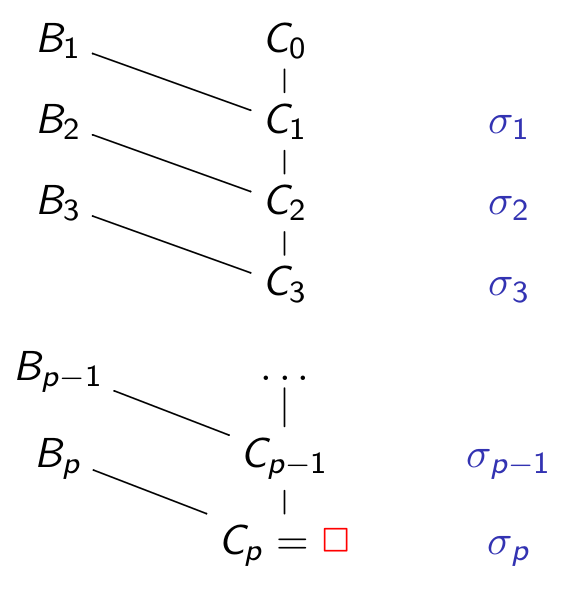
\includegraphics[scale=0.25]{img/resol/lineal.png}
    \end{center}

    donde $C_0$ y cada $B_i$ es un elemento de $S$ (o algún $C_j$ con $j < i$)

    En cada paso agarramos el último resolvente y lo intentamos de resolver
    contra alguno del conjunto de cláusulas o alguno de los resolventes
    anteriores.
\end{definition*}

\begin{example*}Ejemplo de resolución lineal
    \begin{center}
        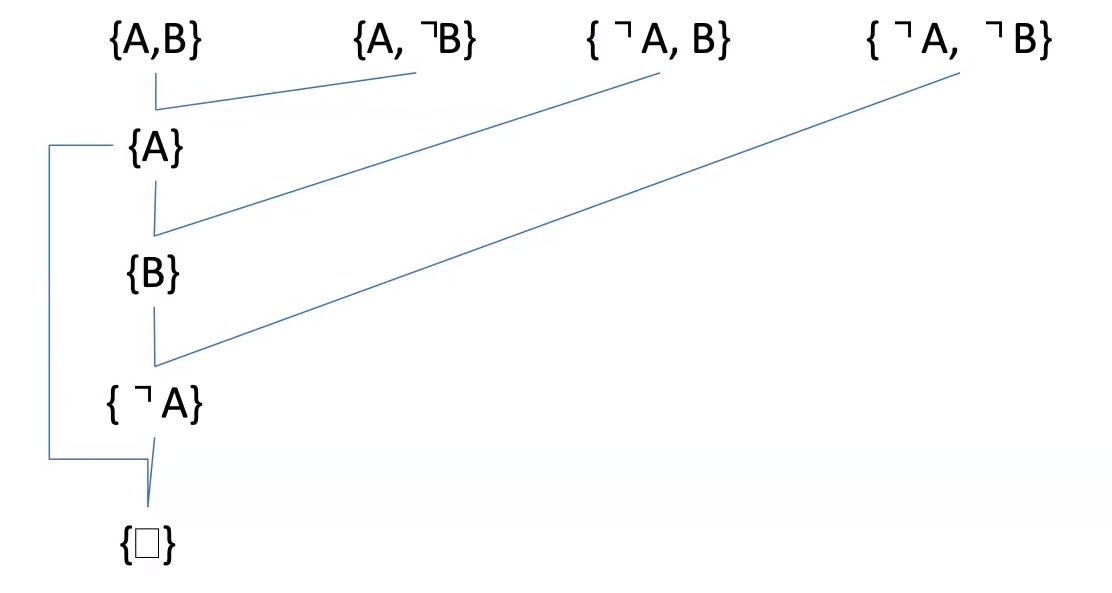
\includegraphics[scale=0.25]{img/resol/lineal-ex.png}
    \end{center}
\end{example*}

Características

\begin{itemize}
    \item En general \textbf{reduce} el espacio de búsqueda considerablemente
    (restringimos que cláusulas podemos elegir)
    \item Preserva \textbf{completitud} (si la fórmula es insatisfactible,
    existe una resol lineal que llega a una refutación).
    \item Pero sigue siendo muy \textbf{no determinístico}. El criterio de
    búsqueda deja espacio para refinamientos y no se especificó ningún criterio
    de selección.
\end{itemize}

\subsection{Cláusulas de Horn}

\begin{nota}
Es un mecanismo que nos va a dar mayor eficiencia en el proceso de producir
refutaciones, sin perder completitud, pero usando \textit{subclases} de
fórmulas. Una subclase es las \textbf{cláusulas de Horn}, que son disyunciones
de literales que tienen \textbf{a lo sumo} un literal positivo.

Las formas clausales (\fullref{sec:logico:resol-lpo:clausal}) tenían la
siguiente pinta
\[
    \forall x_{11}\dots \forall x_{1m_1} .C_1 \wedge \dots \wedge
    \forall x_{k1}\dots \forall x_{km_k} .C_k
\]

una conjunción de \textbf{cláusulas} $\forall x_1 \dots \forall x_m C$ donde cad
$C$ es una disyunción de literales, y se escribían como $\set{C_1', \dots,
C_k'}$ donde cada $C_i'$ es el conjunto de literales en $C_i$.
\end{nota}

\begin{definition*}[Cláusula de Horn]
    Las \textbf{cláusulas de Horn} son de la forma
    $\forall x_1, \dots \forall x_m C$ tal que la disyunción de literales $C$
    tiene \textbf{a lo sumo} un literal positivo.

    C puede tomar una de las formas,
    \begin{itemize}
        \item $\set{B, \no{A_1}, \dots, \no{A_n}}$ (cláusula de definición)
        \item $\set{B}$ (verdades o hechos)
        \item $\set{\no{A_1}, \dots, \no{A_n}}$ (clausula \textbf{goal},
        objetivo o negativa)
    \end{itemize}
\end{definition*}

\textbf{No} toda fórmula de primer orden puede expresarse como una cláusula de
Horn, por ejemplo,

\begin{itemize}
    \item $\paratodo{x}{(P(x) \vee Q(x))}$ (tiene dos literales positivos)
    \item \(
    \impl
    {
        \paratodo{x}{P(x)}
        \vee
        \paratodo{x}{Q(x)}
    }
    {
        \paratodo{x}{(P(x) \vee Q(x))}
    }
    \)
\end{itemize}

Sin embargo, es suficientemente expresivo como para representar programas en la
visión de resolución como cómputo (lo vemos en Prolog).

\subsubsection{Tipos de cláusulas}

Una \textbf{cláusula de definición} (definite clause) es una de la forma
$\forall x_1 \dots \forall x_m C$ tal que la disyunción de literales $C$
tiene \textit{exactamente} un literal positivo.

Y sea $S = P \cup \set{G}$ un conjunto de cláusulas de Horn (con nombres de
vars disjuntos) tal que $P$ es un conjunto de cláusulas de definición y $G$
una negativa, decimos que son las \textbf{cláusulas de entrada}.

Donde,
\begin{itemize}
    \item $P$ se conoce como \textbf{el programa o base de conocimientos}, y
    \item $G$ es el \textbf{goal}, \textbf{meta} o \textbf{cláusula
    objetivo}
\end{itemize}

\subsection{Resolución SLD}

\begin{nota}
    S: Selectiva
    L: Lineal
    D: Definición
    (Selective Linear Definite)
\end{nota}

Una secuencia de pasos de \textbf{resolución SLD} para $S$ es una secuencia
\[
\langle
    N_0, N_1, \dots, N_p
\rangle
\]
de \textbf{cláusulas negativas} que satisfacen dos condiciones,

\begin{enumerate}
    \item $N_0$ es el goal $G$
    \item Para todo $N_i$ en la secuencia, $0 < i < p$, si $N_i$ es
    \[
        \set{
            \no{A_1}, \dots, \no{A_{k-1}}, \no{A_k},
            \no{A_{k+1}, \dots, \no{A_n}}
        }
    \]

    entonces hay alguna \textbf{cláusula de definición} $C_i$ de la forma
    $\set{A, \no{B_1}, \dots, \no{B_m}}$ en $P$ tal que $A_k$ y $A$ son
    unificables con un MGU $\sigma$, y si
    \begin{itemize}
        \item $m = 0$ (i.e es una \textit{verdad}) entonces $N_{i+1}$ es
        
        \(
            \sigma(\set{
                \no{A_1}, \dots, \no{A_{k-1}},
                \no{A_{k+1}, \dots \no{A_n}}
            })
        \)
        \item $m > 0$ entonces $N_{i+1}$ es
        
        \(
            \sigma(\set{
                \no{A_1}, \dots, \no{A_{k-1}},
                \no{B_1}, \dots, \no{B_m},
                \no{A_{k+1}, \dots \no{A_n}}
            })
        \)
    \end{itemize}
\end{enumerate}

\subsection{Refutación SLD}

y entonces una \textbf{refutación SLD} es una secuencia de pasos de resolución
SLD $\langle N_0, \dots, N_p \rangle$ tal que $N_p = \changed{\emptyCl}$ (llega
a una cláusula vacía)

\begin{center}
    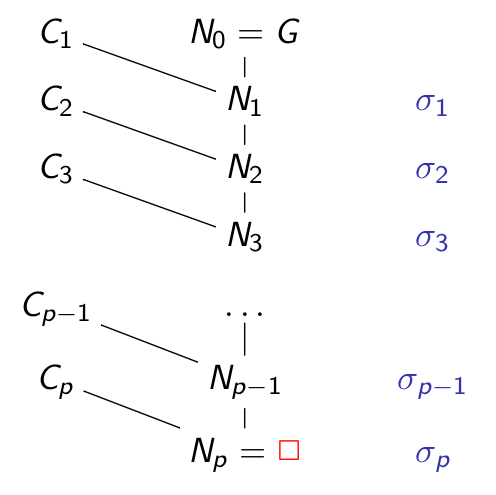
\includegraphics[scale=0.25]{img/resol/refutacion-sld.png}
\end{center}

De esa forma,

\begin{itemize}
    \item En cada paso, se resuelven las cláusulas \(
        \set{
            \no{A_1}, \dots, \no{A_{k-1}}, \no{A_k},
            \no{A_{k+1}, \dots, \no{A_n}}
        }
    \) (resolvente anterior) y $\set{A, \no{B_1}, \dots, \no{B_m}}$ (definición)

    \item Los átomos $A_k$ y $A$ se unifican con un MGU $\sigma_i$
    \item El literal $A_k$ se llama \textbf{átomo seleccionado} de $N_i$
    \item Al final, tenemos la \textbf{sustitución respuesta}
    \[
        \sigma_p \circ \dots \circ \sigma_1
    \]
    (esta se usa en Prolog para extraer la salida del programa)
\end{itemize}

\subsubsection{Ejemplo}

Consideremos las siguientes cláusulas de definición,

\begin{itemize}
    \item $C_1 = \set{add(U, 0, U)}$
    \item $C_2 = \set{add(X, succ(Y), succ(Z)),\ \neg add(X, Y, Z)}$
\end{itemize}

y la cláusula goal
\[
    \set{\neg add(succ(0), V, succ(succ(0)))}
\]

queremos mostrar que el conjunto de estas cláusulas $\set{C_1, C_2, G}$ es
insatisfactible.

\begin{center}
    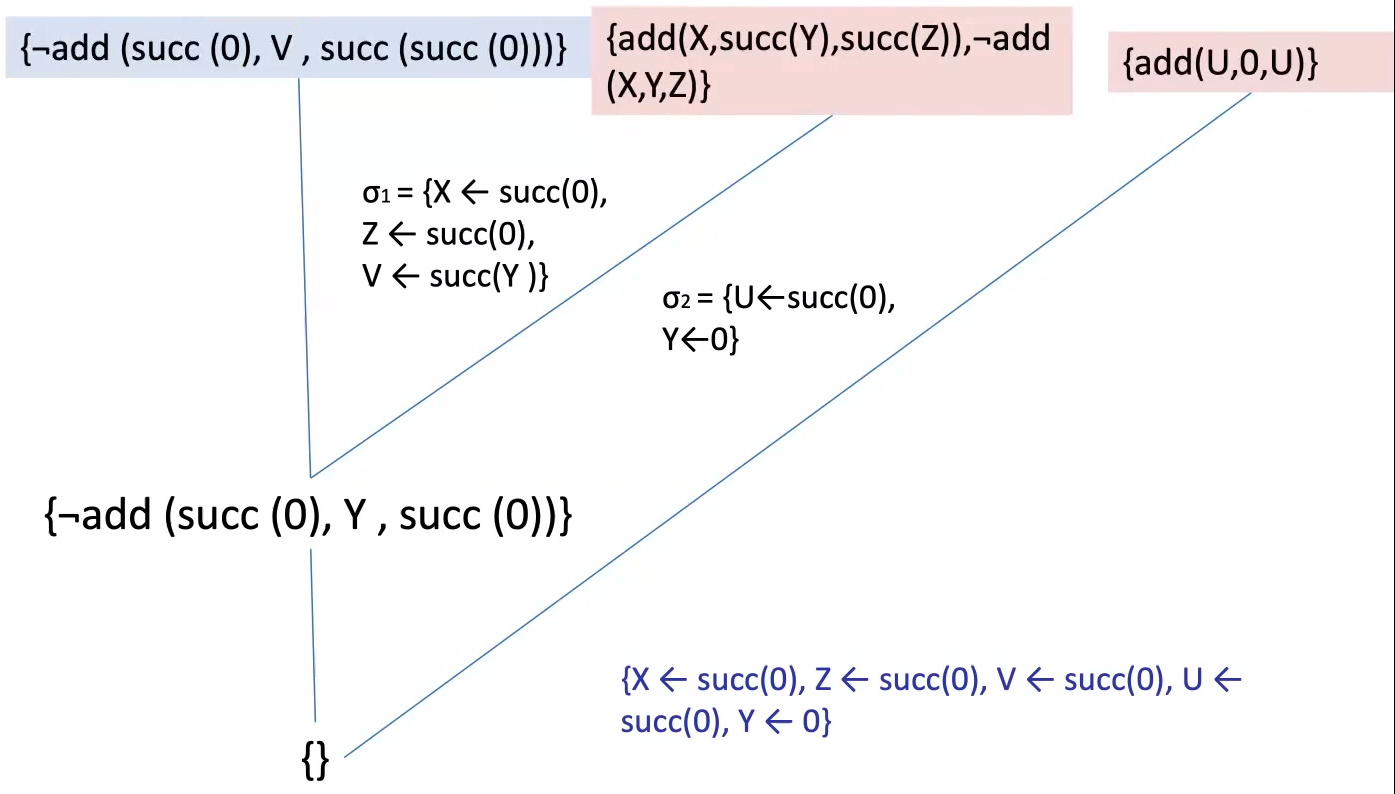
\includegraphics[scale=0.25]{img/resol/resol-sld-ex.png}
\end{center}

Y 

\begin{center}
    \begin{tabular}{ lll }
        \textbf{Cláusula goal}                      & \textbf{Cláusula de entrada} & \textbf{Sust} \\
        $\set{\neg add(succ(0), V, succ(succ(0)))}$ & $C_2$                        &               \\
        $\set{\neg add(succ(0), Y, succ(0))}$       & $C_1$                        & $\sigma_1$    \\
        $\changed{\emptyCl}$                        &                              & $\sigma_2$
    \end{tabular}
\end{center}

donde
\begin{align*}
    \sigma_1 &= \set{\sust{X}{succ(0)}, \sust{V}{succ(Y)}, \sust{Z}{succ(0)}}\\
    \sigma_2 &= \set{\sust{U}{succ(0)}, \sust{Y}{0}}
\end{align*}

y la sustitución resultado es
\begin{align*}
    \comp{\sigma_2}{\sigma_1} =
    \set{
        &\sust{X}{succ(0)},\\
        &\sust{V}{succ(0)},\\
        &\sust{Z}{succ(0)},\\
        &\sust{U}{succ(0)},\\
        &\sust{Y}{0}
    }
\end{align*}

\subsection{Corrección y completitud}

\begin{itemize}
    \item \textbf{Corrección}: Si un conjunto de cláusulas de Horn tiene una
    refutación SLD, entonces es insatisfacible.

    \item \textbf{Completitud}: Si un conjunto de cláusulas de Horn $P \cup
    \set{G}$ como fue descrito, si es insatisfacible, existe una refutación SLD
    cuya primera cláusula es G.
\end{itemize}

\begin{nota}
    Si el algoritmo de resolución original era correcto, entonces este
    también, ya que impone restricciones y se aplica sobre un subconjunto de
    las fórmulas.

    La completitud se preserva solamente para cláusulas de Horn.
\end{nota}

\section{Prolog}

\begin{example*} Ejemplo de programa de prolog
    \begin{minted}{prolog}
    % Hechos
    habla(ale, ruso).
    habla(juan, ingles).
    habla(maria, ruso).
    habla(maria, ingles).

    % Reglas de inferencia
    seComunicaCon(X, Y) :- habla(X, L), habla(Y, L), X \= Y.

    % Ejemplo de goal
    seComunicaCon(X, ale)
    % X = maria
    seComunicaCon(X, Y)
    % X = maria, Y = juan y le podemos pedir más
    \end{minted}

    Depende de como instancie un goal, puede funcionar distinto

\end{example*}

\subsection{Resolución SLD en Prolog}

Prolog usa resolución SLD con las siguientes restricciones:

\begin{itemize}
    \item \textbf{Regla de búsqueda}: se seleccionan las cláusulas del programa
    de arriba hacia abajo, en el orden que fueron introducidas.
    \item \textbf{Regla de selección}: se selecciona el átomo de más a la
    izquierda.
\end{itemize}

La suma de ambas se llama \textbf{estrategia}, y cada una determina un árbol de
búsqueda o \textbf{árbol SLD} distinto.

\begin{nota}
    Sobre la regla de selección, nosotros tenemos un super goal que puede tener
    muchos literales negados, y selecciona el que está más a la izquierda (nos
    da determinismo). Esto permite que alteremos el orden el que aparecen las
    cosas según como queremos que ejecute.
\end{nota}

\begin{example*}
Ejemplo de resolución SLD en Prolog

Cláusulas de definición:
\begin{enumerate}
    \item $\set{p(X, Z), \neg q(X, Y), \neg p(Y, Z)}$
    \item $\set{p(X, X)}$
    \item $\set{q(a, b)}$
\end{enumerate}

Cláusula goal: $\set{\neg p(X, b)}$

El árbol de búsqueda seleccionando el átomo que está más a la izquierda es

\begin{center}
    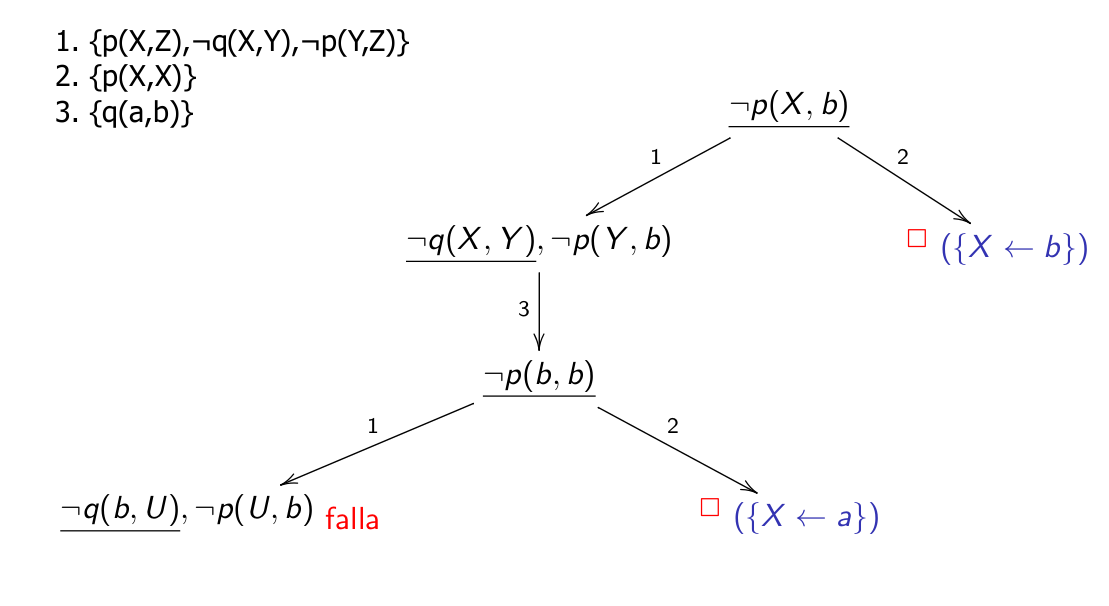
\includegraphics[scale=0.3]{img/prolog/prolog-sld-left-ex.png}
\end{center}
\begin{enumerate}
    \item Camino 1: 
    \begin{itemize}
        \item $\sigma_1 = \set{\sust{Z}{b}}$
        \item $\sigma_2 = \set{\sust{X}{a}, \sust{Y}{b}}$
        \item $\sigma_3 = \set{\sust{X}{b}}$
    \end{itemize}
    La sustitución final es
    $\sigma_3 \circ \sigma_2 \circ \sigma_1 = \set{\sust{Z}{b}, \sust{X}{a},
    \sust{y}{b}}$.

    (tiene prioridad el $\sust{X}{a}$ por sobre el $\sust{X}{b}$ por como se
    comporta la composición de sustituciones, ver
    \fullref{sec:func:inferencia:unif:comp})

    \item Camino 2: lleva directo a $\sigma_1 = \set{\sust{X}{b}}$.
\end{enumerate}
\end{example*}

\subsubsection{Variando estrategia}

Se podría variar la \textbf{regla de selección} para que elija el átomo de más a
la derecha por ejemplo, lo que llevaría a un árbol SLD distinto.

\begin{example*} Eligiendo el átomo de más a la derecha
    \begin{center}
        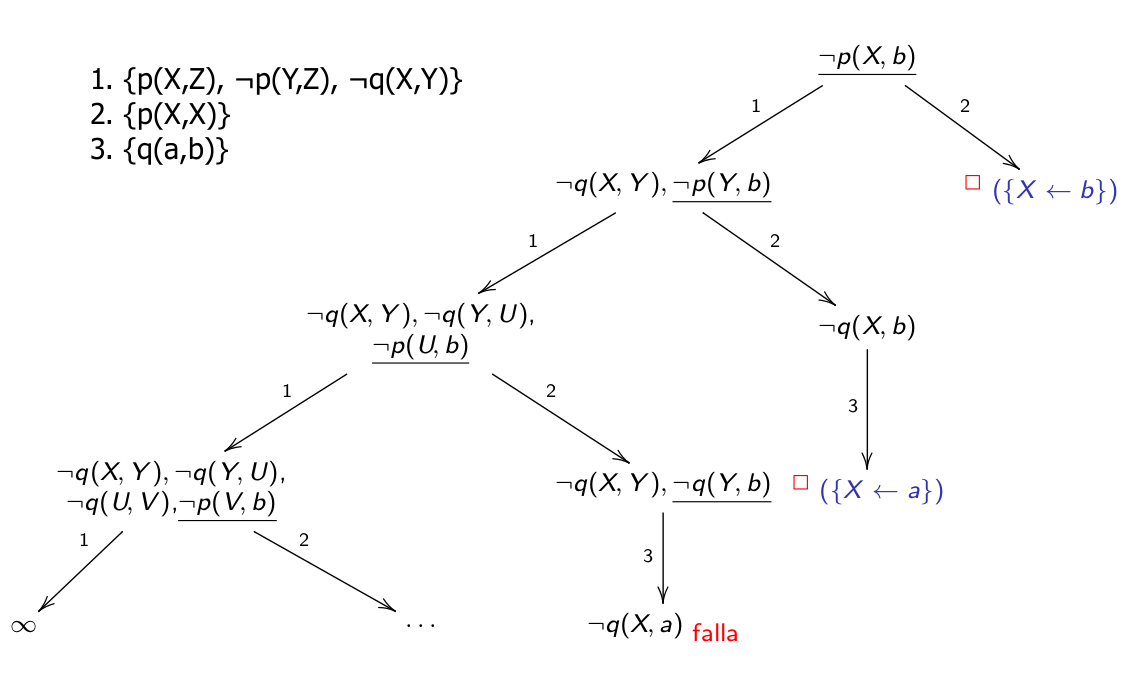
\includegraphics[scale=0.3]{img/prolog/prolog-sld-right-ex.png}
    \end{center}

    nos puede pasar que el árbol diverge, lo cual no quiere decir que no pueda
    encontrar soluciones.
\end{example*}

También se podría variar la regla de búsqueda, en cuyo caso también podría
variar el árbol SLD asociado. Por ejemplo, podría seleccionar las cláusulas de
abajo hacia arriba en vez de arriba hacia abajo.

La importancia de entender la estrategia que se usa (en Prolog) es que podemos
estructurar nuestro programa para tener mejores árboles SLD (y que sea más
eficiente).

\subsection{Motivación de resolución SLD como cómputo}

Vamos a explorar de qué manera la \textbf{resolución SLD} puede usarse para
\textbf{computar}. Además vemos el rol de la \textbf{sustitución respuesta} como
``resultado del cálculo''.

Vamos a especificar con fórmulas un cómputo, hacer una pregunta y mediante
resolución vamos a obtener una sustitución que es la respuesta.

Recordando el ejemplo de la suma, que puede verse como una definición recursiva
de la suma,

\begin{itemize}
    \item $C_1 = \set{add(U, 0, U)}$ 

    ($U + 0 = U$)
    \item $C_2 = \set{add(X, succ(Y), succ(Z)),\ \neg add(X, Y, Z)}$

    (si $X+Y = Z$, entonces $X + succ(Y) = succ(Z)$)
\end{itemize}

Y queremos saber si, dada esa definición, ``Existe $V$ tal que $1 + V = 2$?''

\[
    \existe{V}{add(succ(0), V, succ(succ(0)))}
\]

Esto podemos plantearlo como la \textbf{validez} de la fórmula

\[
    \impl{C_1 \wedge C_2}{
        \existe{V}{add(succ(0), V, succ(succ(0)))}
    }
\]

(la definición de la suma implica que existe un valor tal que 1 + el da 2)

es decir,

\[
    \impl
    {
        \ubrace{C_1 \wedge C_2}{\text{Define la suma}}
    }
    {
        \ubrace{
            \existe{V}{add(succ(0), V, succ(succ(0)))}
        }{\text{Pide calcular } V}
    } \text{ es válida}
\]

que es lo mismo que preguntarse por la \textbf{insatisfactibilidad} de la
negación
\begin{align*}
    &\neg (\impl{C_1 \wedge C_2}{
        \existe{V}{add(succ(0), V, succ(succ(0)))}
    })\\
    \iff &\neg (
        \neg (C_1 \wedge C_2) \vee \existe{V}{add(succ(0), V, succ(succ(0)))}
    )\\
    \iff &C_1 \wedge C_2 \wedge \neg\existe{V}{add(succ(0), V, succ(succ(0)))}\\
    \iff &C_1 \wedge C_2 \wedge
        \paratodo{V}{\neg add(succ(0), V, succ(succ(0)))}
\end{align*}
Que son tres cláusulas, y lo podemos escribir como
\begin{align*}
    \Big\{
        &\set{add(U, 0, U)},\\
        &\set{add(X, succ(Y), succ(Z)), \neg add(X, Y, Z)},\\
        &\set{\neg add(succ(0), V, succ(succ(0)))}
    \Big\}
\end{align*}

y con ese conjunto de cláusulas disparamos la resolución SLD. Si tiene éxito,
con la sustitución respuesta obtenemos un valor para el $V$ buscado. Es
importante observar que no solo nos interesa saber que exista ese $V$, queremos
una instancia del mismo.

\subsection{Notación Prolog}

\begin{nota}
    La resolución SLD partía de un conjunto de cláusulas $S = P \cup \set{G}$
    donde
    
    \begin{enumerate}
        \item $P$ es un conjunto de cláusulas \textbf{definición}, cláusulas con
        exactamente un literal positivo.
        \begin{gather*}
            \set{B, \neg A_1, \dots, \neg A_n}\\
            \set{B}
        \end{gather*}
        \item $G$ es un \textbf{goal}, una cláusula negativa
        \[
            \set{\neg A_1, \dots, \neg A_n}
        \]
    \end{enumerate}
\end{nota}

Notar que
\begin{align*}
    B \vee \neg A_1 \vee \dots \vee \neg A_n
    \iff &\neg(A_1 \wedge \dots \wedge A_n) \vee B\\
    \iff &\impl{(A_1 \wedge \dots \wedge A_n)}{B}
\end{align*}
como consecuencia, las cláusulas en $P$ definen implicaciones o cosas que son
verdaderas y se escriben
\begin{itemize}
    \item $B :- A_1, \dots, A_n.$ para
    $\set{B, \neg A_1, \dots, \neg A_n}$ (\textbf{reglas})
    \item $B.$ para $\set{B}$ (\textbf{hechos})
\end{itemize}

\subsection{Ejemplos}

\subsubsection{Suma}

El ejemplo de la suma en Prolog se escribiría como
\begin{minted}{prolog}
    add(U, 0, U).
    add(X, succ(Y), succ(Z)) :- add(X, Y, Z).

    % Ingresamos el goal
    ?- add(succ(0), V, succ(succ(0)))

    % La respuesta es
    V = succ(0)
\end{minted}

\subsubsection{Familiares}

\begin{minted}{prolog}
    hijo(fred, sally).
    hijo(tina, sally).
    hijo(sally, john).
    hijo(sally, diane).
    hijo(sam, bill).
    hermanos(A, B) :- hijo(P, A), hijo(P, B), A \= B.
\end{minted}

Si el goal es \texttt{hermanos(john, X)}, entonces la refutación SLD para $P
\wedge \paratodo{X}{\neg hermanos(john, X)}$ nos va a dar la sustitución respuesta
$\sigma = \set{\sust{X}{diane}}$

Puede que la sustitución respuesta asigne valores a variables intermedias que
surgieron en el proceso de búsqueda de una refuctación.

Secuencia SLD:

\begin{enumerate}
    \item $\set{hijo(fred, sally)}$
    \item $\set{hijo(tina, sally)}$
    \item $\set{hijo(sally, john)}$
    \item $\set{hijo(sally, diane)}$
    \item $\set{hijo(sam, bill)}$
    \item $\set{hermanos(A, B),\neg hijo(P, A),\neg hijo(P, B),\neg A \neq B}$
    \item (goal) $\neg hermanos(john, X)$
    \item (7 y 6)
    $\set{\neg hijo(P, john),\neg hijo(P, B),\neg john \neq B}$
    
    $\sigma = \set{\sust{A}{john}, \sust{X}{B}}$
    \item (8 y 3)
    $\set{\neg hijo(sally, B), \neg john \neq B}$
    
    $\sigma = \set{\sust{P}{sally}}$
    \item (9 y 4)
    $\set{john = diane}$
    
    $\sigma = \set{\sust{B}{diane}}$
    \item $\changed{\emptyCl}$
    
    \todo{Acá no estoy seguro de como es, pero supongo que como $john = diane$
    es falso queda la cláusula vacía}
\end{enumerate}

la sustitución resultado es
$\sigma = \set{
    \sust{A}{john},
    \select{\sust{X}{diane}},
    \sust{P}{sally},
    \sust{B}{diane}
}$

\subsection{Corrección y completitud}

\textbf{Corrección}: Si existe una refutación SLD de $P \cup \set{G}$ con la
estrategia de antes, entonces es insatisfactible.

\textbf{Completitud}: Si $P \cup \set{G}$ es insatisfactible, entonces existe
una refutación SLD con la estrategia de antes a partir del él.

\subsection{Refuctaciones SLD en Prolog}

Prolog recorre el árbol SLD en \textbf{profundidad} (hace DFS). La ventaja es
que puede ser implementado de manera muy eficiente,

\begin{itemize}
    \item Se usa una \textbf{pila} para representar los átomos del goal
    \item Se hace \textbf{push} del resolvente del átomo del tope de la pila con
    la cláusula de definición
    \item Se hace \textbf{pop} cuando el átomo del tope de la pila no unifica
    con ninguna cláusula de definición más. Luego, el átomo que queda en el tope
    se unifica con la siguiente cláusula de definición.
\end{itemize}

Pero tiene como desventaja que puede que no encuentre una resolución SLD aún si
existe.

\subsection{Aspectos extra lógicos}

Dos temas de Prolog que trascienden la lógica subyacente:

\begin{enumerate}
    \item \textbf{Cut}: No permiten controlar como se crea el árbol de
    resolución (podarlo o hacerlo más eficiente)
    \item Deducción de información negativa, negation as failure
    (\textbf{negación por falla}): cómo podemos inferir información sobre cosas
    que \textit{no} pasan
\end{enumerate}

\subsubsection{Cut}

Es un predicado 0-ario \changed{\textbf{!}} que solo tiene éxito la primera vez
que se lo invoca (no podes pasar de vuelta por ahí, limita las opciones de
backtracking). Brinda un mecanismo de control que permite hacer
\textit{prunning} del árbol SLD (podar).

Es extra lógico (no se corresponde con un predicado estándar de LPO), y está por
cuestiones de eficiencia. Pero hay que tener cuidado, porque puede podarse una
rama de éxito deseada.

\begin{example*}Ejemplo de cut
\begin{minted}{prolog}
    p(a).
    p(b).
    p(c).
    q(a, e).
    q(a, f).
    q(b, f).

    % Consultas

    ?- p(X).
    X = a; X = b; X = c;
    no

    ?- p(X), !.
    X = a;
    no
    % p(X) va a resolver a cut, que la primera vez tiene éxito, pero elimina
    % las posibilidades de hacer backtracking por lo que no puede resolver p(X)
    % para otros X.

    ?- p(X), q(X, Y).
    X = a, Y = e;
    X = a, Y = f;
    X = b, Y = f;
    no

    ?- p(X), !, q(X, Y).
    X = a, Y = e;
    X = a, Y = f;
    no
    % Acá es lo mismo, pero la resolvente es !, q(X, Y), porque lo que se puede
    % hacer backtracking qué resolver q(X, Y), pero no sobre qué resolver p(X)
\end{minted}
\end{example*}

\begin{example*}Otro ejemplo
    \begin{minted}{prolog}
    p(a).
    p(b).
    p(c).
    q(a, e).
    q(a, f).
    q(b, f).
    r(X, Y) :- p(X), !, q(X, Y).

    % Consultas

    ?- r(X, Y).
    X = a, Y = e;
    X = a, Y = f;
    no

    ?- p(X), r(X, Y).
    X = a, Y = e;
    X = a, Y = f;
    X = b, Y = f;
    no
    % No mata las opciones del p(X) de "arriba".
    % Podas la rama de la cláusula definición donde aparece el cut, pero no
    % de más arriba.
    \end{minted}
    
\end{example*}

Esto funciona así porque \textbf{las ramas que se podan son la de la cláusula de
definición donde aparece el cut, pero no de más arriba}.

\begin{nota}
    Por ej. si tenemos \texttt{p(X), s(Y), !, q(X, Y)} (suponiendo que s(e),
    s(f)) el ! también cortaría esas posibilidades.
    \begin{minted}{prolog}
    ?- p(X), s(Y), q(X, Y).
    X = a, Y = e ;
    X = a, Y = f ;
    X = b, Y = f ;
    false.

    ?- p(X), s(Y), !, q(X, Y).
    X = a, Y = e ;
    false.
    \end{minted}
\end{nota}

\begin{example*}
    Definición de max
    \begin{minted}{prolog}
    max1(X, Y, Y) :- X =< Y.
    max1(X, Y, X) :- X > Y.

    % Consulta
    ?- max1(3, 4, Z).
    Z = 4;
    false. % No queremos que pruebe más!
    \end{minted}

    es ineficiente, porque puede intentar de buscar más soluciones. Uno puede
    usar cut para sacarse de encima este problema.

    \begin{minted}{prolog}
    max2(X, Y, Y) :- X =< Y, !.
    max2(X, Y, X) :- X > Y.

    % Consulta
    ?- max2(3, 4, Z).
    Z = 4.
    \end{minted}

    otra opción más,

    \begin{minted}{prolog}
    max3(X, Y, Y) :- X =< Y, !.
    max3(X, Y, X).

    % Consulta
    ?- max3(3, 4, Z).
    Z = 4.

    % Pero no es válido, porque acá devuelve true de una en vez de ver la otra
    ?- max2(2, 3, 2).
    true. % pero es falso esto
    % no puede unifcar con la primera, entonces unifica con la 2da de una.
    \end{minted}
\end{example*}

En general,

\begin{itemize}
    \item Cuando se selecciona un cut, tiene éxito inmediatamente
    \item Si debido al backtracking se vuelve a ese cut, su efecto es hacer
    fallar el goal que le dio origen. (el goal que unificó con la cabeza de la
    cláusula que \textbf{contiene} al corte y que hizo que esa cláusula se
    activara)
    \item El efecto obtenido es el de \textbf{descartar soluciones} (no dar más)
    de
    \begin{enumerate}
        \item otras cláusulas del goal padre
        \item cualquier goal que ocurre a la izquierda del corte en la cláusula
        que contiene el corte
        \item todos los objetivos intermedios que se ejecutaron durante la
        ejecución de los goals precedentes.
    \end{enumerate}
\end{itemize}

\begin{nota}
    Otra forma de verlo, sacada de
    \href{https://www.cse.iitb.ac.in/~cs206/lecs/lec17.pdf}{CS206 Lecture 16}.

    El \textbf{Goal padre} (\textit{parent goal}) es el goal que matcheo con la
    cabeza de la cláusula que contiene el cut.

    Cuando un cut es encontrado, se \textbf{resuelve} inmediatamente.

    El \textbf{efecto} del cut es que el sistema se comprometa (\textit{commit})
    a todas las elecciones realizadas desde el momento en el que el goal padre
    se llamó hasta que se resolvió el cut (incluyendo al goal padre). Es decir,
    todas alternativas pendientes entre el goal padre y el cut se descartan.

    Por ejemplo, si tenemos

    \begin{minted}{prolog}
    C :- P, Q, R, !, S, T, U.
    C :- V.
    A :- B, C, D.
    \end{minted}

    Cuando se intenta de resolver A, intentamos C luego de obtener la primera
    solución para B. Acá se resuelven de a una P, Q, R y se encuentra el cut,
    que se resuelve inmediatamente. En este momento la resolución se
    "compromete" a las elecciones realizadas para P, Q y R y no va a
    backtrackear para buscar otras. Tampoco va a intentar matchear C con otra
    cabeza, por ejemplo \texttt{C :- V}. Pero si va a devolver todas las nuevas
    respuestas obtenidas de S, T y U.

    El cut es invisible a A, y todas las opciones de B y D se van a probar.
\end{nota}

\subsubsection{Not - Negación por falla}

En cláusulas de Horn no hay una forma directa de escribir negaciones. Si uno las
traduce, significan que un hecho es true.

Dado un árbol SLD, podemos tener ramas de falla. Si tenemos un árbol que falla
\textbf{finitamente} (tiene ramas de falla finitas y no tiene ramas de éxito)

Dado un programa P el \textbf{conjunto de falla finita} de P es
\[
    \set{B \mid B \text{ es átomo cerrado ('ground') y existe un árbol SLD que falla finitamente con B como raíz}}
\]

Un átomo cerrado es uno que no tiene variables, por ej. $P(a)$ a dif de $P(x)$.

Infiere la regla de negation as failure
\[
    \resol
    {
        \text{$B$ átomo cerrado}
        \quad
        \text{$B$ en conjunto de falla finita de $P$}
    }
    {\neg B}
\]

Esto en prolog se implementa con el \textbf{predicado not},
\begin{minted}{prolog}
not(G) :- G, !, fail.
not(G).
\end{minted}

not(G) matchea con el primero. Llamá a G. Si encontraste algo en tu base de
conocimiento que lo resuelve, cortá (cut) y fallá. Pero si no encontraste nada,
el primero falla, y la 2da definición da true.

En otras palabras, si tenés éxito fallás y si fallás tenés éxito.

\begin{nota}
    Es importante que not(G) contenga cut (!). De no ser así, siempre devolvería
    true, ya que aunque falle para la primera luego resolvería por la segunda.

    Se puede probar implementando
    \begin{minted}{haskell}
        not2(G) :- G, fail
    \end{minted}
\end{nota}

\begin{example*}
    Podemos deducir \texttt{not(student(mary))} y \texttt{not(student(anna))} a
    partir de
    \begin{minted}{prolog}
    student(joe).
    student(bill).
    student(jim).
    teacher(mary).
    \end{minted}
\end{example*}

Pero negación por falla \textbf{no es la negación lógica}

\begin{example*} Por ejemplo
    \begin{minted}{prolog}
    animal(perro).
    animal(gato).
    vegetal(X) :- not(animal(X)).
    \end{minted}

    La consulta \texttt{vegetal(perro)} da no como se espera, idem
    \texttt{vegetal(pasto)} que da si.
    
    Pero \texttt{vegetal(X)} da falso. (porque no es un átomo cerrado).
\end{example*}

Para que estos predicados funcionen, es necesario que esté instanciado lo que
quiero negar. El goal \texttt{not(G)} \textbf{nunca instancia variables} de $G$.

\begin{itemize}
    \item Si G tiene éxito, \texttt{fail} falla y descarta la sustitución
    \item Caso contrario, \texttt{not(G)} tiene éxito inmediatamente (sin
    afectar ni contrar sustituciones para G).
\end{itemize}

por lo tanto, \texttt{not(not(animal(X)))} no es equivalente a
\texttt{animal(X)}, da true.

\begin{nota}
    Porque
    \begin{verbatim}
    not(not(animal(X)))
    (G = not(animal(X)))
    not(animal(X)), !, fail
    \end{verbatim}
    y como \texttt{not(animal(X))} da false, el G de arriba falló, y not tenía
    éxito cuando G fallaba, por lo que el not de arriba tiene éxito y el
    resultado total es \texttt{true}.
\end{nota}

\begin{example*} Otro ejemplo
    \begin{minted}{prolog}
    firefighter_candidate(X) :-
        not(pyromaniac(X)),
        punctual(X).
    pyromaniac(attila).
    punctual(jeanne_d_arc).

    firefighter_candidate2(X) :-
        punctual(X),
        not(pyromaniac(X)).
    
    ?- firefighter_candidate(W).
    false.
    
    ?- firefighter_candidate2(W).
    W = jeanne_d_arc.
    \end{minted}

    El resultado de \texttt{firefighter\_candidate(W)} es false, porque estoy
    llamando al \texttt{not} sin el X instanciado. En cambio, en
    \texttt{firefighter\_candidate2(W)} como primero instancia el X con punctual,
    el not se llama con X instanciado y funciona como es esperado
\end{example*}

\end{document}

